\documentclass[twoside]{book}

% Packages required by doxygen
\usepackage{fixltx2e}
\usepackage{calc}
\usepackage{doxygen}
\usepackage[export]{adjustbox} % also loads graphicx
\usepackage{graphicx}
\usepackage[utf8]{inputenc}
\usepackage{makeidx}
\usepackage{multicol}
\usepackage{multirow}
\PassOptionsToPackage{warn}{textcomp}
\usepackage{textcomp}
\usepackage[nointegrals]{wasysym}
\usepackage[table]{xcolor}

% Font selection
\usepackage[T1]{fontenc}
\usepackage[scaled=.90]{helvet}
\usepackage{courier}
\usepackage{amssymb}
\usepackage{sectsty}
\renewcommand{\familydefault}{\sfdefault}
\allsectionsfont{%
  \fontseries{bc}\selectfont%
  \color{darkgray}%
}
\renewcommand{\DoxyLabelFont}{%
  \fontseries{bc}\selectfont%
  \color{darkgray}%
}
\newcommand{\+}{\discretionary{\mbox{\scriptsize$\hookleftarrow$}}{}{}}

% Page & text layout
\usepackage{geometry}
\geometry{%
  a4paper,%
  top=2.5cm,%
  bottom=2.5cm,%
  left=2.5cm,%
  right=2.5cm%
}
\tolerance=750
\hfuzz=15pt
\hbadness=750
\setlength{\emergencystretch}{15pt}
\setlength{\parindent}{0cm}
\setlength{\parskip}{3ex plus 2ex minus 2ex}
\makeatletter
\renewcommand{\paragraph}{%
  \@startsection{paragraph}{4}{0ex}{-1.0ex}{1.0ex}{%
    \normalfont\normalsize\bfseries\SS@parafont%
  }%
}
\renewcommand{\subparagraph}{%
  \@startsection{subparagraph}{5}{0ex}{-1.0ex}{1.0ex}{%
    \normalfont\normalsize\bfseries\SS@subparafont%
  }%
}
\makeatother

% Headers & footers
\usepackage{fancyhdr}
\pagestyle{fancyplain}
\fancyhead[LE]{\fancyplain{}{\bfseries\thepage}}
\fancyhead[CE]{\fancyplain{}{}}
\fancyhead[RE]{\fancyplain{}{\bfseries\leftmark}}
\fancyhead[LO]{\fancyplain{}{\bfseries\rightmark}}
\fancyhead[CO]{\fancyplain{}{}}
\fancyhead[RO]{\fancyplain{}{\bfseries\thepage}}
\fancyfoot[LE]{\fancyplain{}{}}
\fancyfoot[CE]{\fancyplain{}{}}
\fancyfoot[RE]{\fancyplain{}{\bfseries\scriptsize Generated by Doxygen }}
\fancyfoot[LO]{\fancyplain{}{\bfseries\scriptsize Generated by Doxygen }}
\fancyfoot[CO]{\fancyplain{}{}}
\fancyfoot[RO]{\fancyplain{}{}}
\renewcommand{\footrulewidth}{0.4pt}
\renewcommand{\chaptermark}[1]{%
  \markboth{#1}{}%
}
\renewcommand{\sectionmark}[1]{%
  \markright{\thesection\ #1}%
}

% Indices & bibliography
\usepackage{natbib}
\usepackage[titles]{tocloft}
\setcounter{tocdepth}{3}
\setcounter{secnumdepth}{5}
\makeindex

% Packages requested by user
\usepackage{amsmath}

% Hyperlinks (required, but should be loaded last)
\usepackage{ifpdf}
\ifpdf
  \usepackage[pdftex,pagebackref=true]{hyperref}
\else
  \usepackage[ps2pdf,pagebackref=true]{hyperref}
\fi
\hypersetup{%
  colorlinks=true,%
  linkcolor=blue,%
  citecolor=blue,%
  unicode%
}

% Custom commands
\newcommand{\clearemptydoublepage}{%
  \newpage{\pagestyle{empty}\cleardoublepage}%
}

\usepackage{caption}
\captionsetup{labelsep=space,justification=centering,font={bf},singlelinecheck=off,skip=4pt,position=top}

%===== C O N T E N T S =====

\begin{document}

% Titlepage & ToC
\hypersetup{pageanchor=false,
             bookmarksnumbered=true,
             pdfencoding=unicode
            }
\pagenumbering{alph}
\begin{titlepage}
\vspace*{7cm}
\begin{center}%
{\Large Reference Manual}\\
\vspace*{1cm}
{\large Generated by Doxygen 1.8.13}\\
\end{center}
\end{titlepage}
\clearemptydoublepage
\pagenumbering{roman}
\tableofcontents
\clearemptydoublepage
\pagenumbering{arabic}
\hypersetup{pageanchor=true}

%--- Begin generated contents ---
\chapter{Modular arbitrary-\/order ocean-\/atmosphere model\+: M\+A\+O\+O\+AM -\/-\/ Fortran implementation}
\label{index}\hypertarget{index}{}\subsection*{About}

(c) 2013-\/2016 Lesley De Cruz and Jonathan Demaeyer

See \href{../LICENSE.txt}{\tt L\+I\+C\+E\+N\+S\+E.\+txt} for license information.

This software is provided as supplementary material with\+:


\begin{DoxyItemize}
\item De Cruz, L., Demaeyer, J. and Vannitsem, S.\+: The Modular Arbitrary-\/\+Order Ocean-\/\+Atmosphere Model\+: M\+A\+O\+O\+AM v1.\+0, Geosci. Model Dev., 9, 2793-\/2808, \href{http://dx.doi.org/10.5194/gmd-9-2793-2016}{\tt doi\+:10.\+5194/gmd-\/9-\/2793-\/2016}, 2016.
\end{DoxyItemize}

{\bfseries Please cite this article if you use (a part of) this software for a publication.}

The authors would appreciate it if you could also send a reprint of your paper to \href{mailto:lesley.decruz@meteo.be}{\tt lesley.\+decruz@meteo.\+be}, \href{mailto:jonathan.demaeyer@meteo.be}{\tt jonathan.\+demaeyer@meteo.\+be} and \href{mailto:svn@meteo.be}{\tt svn@meteo.\+be}.

Consult the M\+A\+O\+O\+AM \href{http://www.github.com/Climdyn/MAOOAM}{\tt code repository} for updates, and \href{http://climdyn.meteo.be}{\tt our website} for additional resources.

A pdf version of this manual is available \href{../latex/Reference_manual.pdf}{\tt here}. 



\subsection*{Installation}

The program can be installed with Makefile. We provide configuration files for two compilers \+: gfortran and ifort.

By default, gfortran is selected. To select one or the other, simply modify the Makefile accordingly or pass the C\+O\+M\+P\+I\+L\+ER flag to {\ttfamily make}. If gfortran is selected, the code should be compiled with gfortran 4.\+7+ (allows for allocatable arrays in namelists). If ifort is selected, the code has been tested with the version 14.\+0.\+2 and we do not guarantee compatibility with older compiler version.

To install, unpack the archive in a folder or clone with git\+:


\begin{DoxyCode}
1 git clone https://github.com/Climdyn/MAOOAM.git
2 cd MAOOAM
\end{DoxyCode}


and run\+:


\begin{DoxyCode}
1 make
\end{DoxyCode}
 By default, the inner products of the basis functions, used to compute the coefficients of the O\+D\+Es, are not stored in memory. If you want to enable the storage in memory of these inner products, run make with the following flag\+:


\begin{DoxyCode}
1 make RES=store
\end{DoxyCode}


Depending on the chosen resolution, storing the inner products may result in a huge memory usage and is not recommended unless you need them for a specific purpose.

Remark\+: The command \char`\"{}make clean\char`\"{} removes the compiled files.

For Windows users, a minimalistic G\+NU development environment (including gfortran and make) is available at \href{http://www.mingw.org}{\tt www.\+mingw.\+org} . 



\subsection*{Description of the files}

The model tendencies are represented through a tensor called aotensor which includes all the coefficients. This tensor is computed once at the program initialization.


\begin{DoxyItemize}
\item \hyperlink{maooam_8f90}{maooam.\+f90} \+: Main program.
\item \hyperlink{aotensor__def_8f90}{aotensor\+\_\+def.\+f90} \+: Tensor aotensor computation module.
\item I\+C\+\_\+def.\+f90 \+: A module which loads the user specified initial condition.
\item \hyperlink{inprod__analytic_8f90}{inprod\+\_\+analytic.\+f90} \+: Inner products computation module.
\item \hyperlink{rk2__integrator_8f90}{rk2\+\_\+integrator.\+f90} \+: A module which contains the Heun integrator for the model equations.
\item \hyperlink{rk4__integrator_8f90}{rk4\+\_\+integrator.\+f90} \+: A module which contains the R\+K4 integrator for the model equations.
\item Makefile \+: The Makefile.
\item \hyperlink{params_8f90}{params.\+f90} \+: The model parameters module.
\item \hyperlink{tl__ad__tensor_8f90}{tl\+\_\+ad\+\_\+tensor.\+f90} \+: Tangent Linear (TL) and Adjoint (AD) model tensors definition module
\item \hyperlink{rk2__tl__ad__integrator_8f90}{rk2\+\_\+tl\+\_\+ad\+\_\+integrator.\+f90} \+: Heun Tangent Linear (TL) and Adjoint (AD) model integrators module
\item \hyperlink{rk4__tl__ad__integrator_8f90}{rk4\+\_\+tl\+\_\+ad\+\_\+integrator.\+f90} \+: R\+K4 Tangent Linear (TL) and Adjoint (AD) model integrators module
\item \hyperlink{test__tl__ad_8f90}{test\+\_\+tl\+\_\+ad.\+f90} \+: Tests for the Tangent Linear (TL) and Adjoint (AD) model versions
\item R\+E\+A\+D\+M\+E.\+md \+: A read me file.
\item \hyperlink{LICENSE_8txt}{L\+I\+C\+E\+N\+S\+E.\+txt} \+: The license text of the program.
\item \hyperlink{util_8f90}{util.\+f90} \+: A module with various useful functions.
\item \hyperlink{tensor_8f90}{tensor.\+f90} \+: Tensor utility module.
\item \hyperlink{stat_8f90}{stat.\+f90} \+: A module for statistic accumulation.
\item params.\+nml \+: A namelist to specify the model parameters.
\item int\+\_\+params.\+nml \+: A namelist to specify the integration parameters.
\item modeselection.\+nml \+: A namelist to specify which spectral decomposition will be used.
\end{DoxyItemize}





\subsection*{Usage}

The user first has to fill the params.\+nml and int\+\_\+params.\+nml namelist files according to their needs. Indeed, model and integration parameters can be specified respectively in the params.\+nml and int\+\_\+params.\+nml namelist files. Some examples related to already published article are available in the params folder.

The modeselection.\+nml namelist can then be filled \+:
\begin{DoxyItemize}
\item N\+B\+OC and N\+B\+A\+TM specify the number of blocks that will be used in respectively the ocean and the atmosphere. Each block corresponds to a given x and y wavenumber.
\item The O\+MS and A\+MS arrays are integer arrays which specify which wavenumbers of the spectral decomposition will be used in respectively the ocean and the atmosphere. Their shapes are O\+M\+S(\+N\+B\+O\+C,2) and A\+M\+S(\+N\+B\+A\+T\+M,2).
\item The first dimension specifies the number attributed by the user to the block and the second dimension specifies the x and the y wavenumbers.
\item The V\+D\+DG model, described in Vannitsem et al. (2015) is given as an example in the archive.
\item Note that the variables of the model are numbered according to the chosen order of the blocks.
\end{DoxyItemize}

The Makefile allows to change the integrator being used for the time evolution. The user should modify it according to its need. By default a R\+K2 scheme is selected.

Finally, the I\+C.\+nml file specifying the initial condition should be defined. To obtain an example of this configuration file corresponding to the model you have previously defined, simply delete the current I\+C.\+nml file (if it exists) and run the program \+: \begin{DoxyVerb}./maooam
\end{DoxyVerb}


It will generate a new one and start with the 0 initial condition. If you want another initial condition, stop the program, fill the newly generated file and restart \+: \begin{DoxyVerb}./maooam
\end{DoxyVerb}


It will generate two files \+:
\begin{DoxyItemize}
\item evol\+\_\+field.\+dat \+: the recorded time evolution of the variables.
\item mean\+\_\+field.\+dat \+: the mean field (the climatology)
\end{DoxyItemize}

The tangent linear and adjoint models of M\+A\+O\+O\+AM are provided in the \hyperlink{namespacetl__ad__tensor}{tl\+\_\+ad\+\_\+tensor}, rk2\+\_\+tl\+\_\+ad\+\_\+integrator and rk4\+\_\+tl\+\_\+ad\+\_\+integrator modules. It is documented \href{./md_doc_tl_ad_doc.html}{\tt here}.





\subsection*{Implementation notes}

As the system of differential equations is at most bilinear in $y_j$ ( $j=1..n$), $\boldsymbol{y}$ being the array of variables, it can be expressed as a tensor contraction \+:

\[ \frac{d y_i}{dt} = \sum_{j,k=0}^{ndim} \, \mathcal{T}_{i,j,k} \, y_k \; y_j \]

with $y_0 = 1$.

The tensor \hyperlink{namespaceaotensor__def_a0dc43bc9294a18f2fe57b67489f1702f}{aotensor\+\_\+def\+::aotensor} is the tensor $\mathcal{T}$ that encodes the differential equations is composed so that\+:


\begin{DoxyItemize}
\item $\mathcal{T}_{i,j,k}$ contains the contribution of $dy_i/dt$ proportional to $ y_j \, y_k$.
\item Furthermore, $y_0$ is always equal to 1, so that $\mathcal{T}_{i,0,0}$ is the constant contribution to $dy_i/dt$
\item $\mathcal{T}_{i,j,0} + \mathcal{T}_{i,0,j}$ is the contribution to $dy_i/dt$ which is linear in $y_j$.
\end{DoxyItemize}

Ideally, the tensor \hyperlink{namespaceaotensor__def_a0dc43bc9294a18f2fe57b67489f1702f}{aotensor\+\_\+def\+::aotensor} is composed as an upper triangular matrix (in the last two coordinates).

The tensor for this model is composed in the \hyperlink{namespaceaotensor__def}{aotensor\+\_\+def} module and uses the inner products defined in the \hyperlink{namespaceinprod__analytic}{inprod\+\_\+analytic} module.





\subsection*{Final Remarks}

The authors would like to thank Kris for help with the lua2fortran project. It has greatly reduced the amount of (error-\/prone) work.

No animals were harmed during the coding process. 
\chapter{Modular arbitrary-\/order ocean-\/atmosphere model\+: The Tangent Linear and Adjoint model}
\label{md_doc_tl_ad_doc}
\Hypertarget{md_doc_tl_ad_doc}
\subsection*{Description \+:}

The Tangent Linear and Adjoint model model are implemented in the same way as the nonlinear model, with a tensor storing the different terms. The Tangent Linear (TL) tensor $\mathcal{T}_{i,j,k}^{TD}$ is defined as\+:

\[ \mathcal{T}_{i,j,k}^{TL} = \mathcal{T}_{i,k,j} + \mathcal{T}_{i,j,k} \]

while the Adjoint (AD) tensor $\mathcal{T}_{i,j,k}^{AD}$ is defined as\+:

\[ \mathcal{T}_{i,j,k}^{AD} = \mathcal{T}_{j,k,i} + \mathcal{T}_{j,i,k} . \]

where $ \mathcal{T}_{i,j,k}$ is the tensor of the nonlinear model.

These two tensors are used to compute the trajectories of the models, with the equations

\[ \frac{d\delta y_i}{dt} = \sum_{j=1}^{ndim}\sum_{k=0}^{ndim} \, \mathcal{T}_{i,j,k}^{TL} \, y^{\ast}_k \; \delta y_j . \]

\[ -\frac{d\delta y_i}{dt} = \sum_{j=1}^{ndim} \sum_{k=0}^{ndim} \, \mathcal{T}_{i,j,k}^{AD} \, y^{\ast}_k \; \delta y_j . \]

where $\boldsymbol{y}^{\ast}$ is the point where the Tangent model is defined (with $y_0^{\ast}=1$).

\subsection*{Implementation \+:}

The two tensors are implemented in the module \hyperlink{namespacetl__ad__tensor}{tl\+\_\+ad\+\_\+tensor} and must be initialized (after calling \hyperlink{namespaceparams_aa5d1f7f88b00cf3705691de2f6f92a08}{params\+::init\+\_\+params} and \hyperlink{namespaceaotensor__def_a0dc43bc9294a18f2fe57b67489f1702f}{aotensor\+\_\+def\+::aotensor}) by calling \hyperlink{namespacetl__ad__tensor_a8a94fe84e907fc8835f798eddcff38e8}{tl\+\_\+ad\+\_\+tensor\+::init\+\_\+tltensor()} and \hyperlink{namespacetl__ad__tensor_a199cc07a7172f6cf662f9a5bd6f3d45c}{tl\+\_\+ad\+\_\+tensor\+::init\+\_\+adtensor()}. The tendencies are then given by the routine tl(t,ystar,deltay,buf) and ad(t,ystar,deltay,buf). An integrator with the Heun method is available in the module rk2\+\_\+tl\+\_\+ad\+\_\+integrator and a fourth-\/order Runge-\/\+Kutta integrator in rk4\+\_\+tl\+\_\+ad\+\_\+integrator. An example on how to use it can be found in the test file \hyperlink{test__tl__ad_8f90}{test\+\_\+tl\+\_\+ad.\+f90} 
\chapter{Modules Index}
\section{Modules List}
Here is a list of all modules with brief descriptions\+:\begin{DoxyCompactList}
\item\contentsline{section}{\hyperlink{namespaceaotensor__def}{aotensor\+\_\+def} \\*The equation tensor for the coupled ocean-\/atmosphere model with temperature which allows for an extensible set of modes in the ocean and in the atmosphere }{\pageref{namespaceaotensor__def}}{}
\item\contentsline{section}{\hyperlink{namespaceic__def}{ic\+\_\+def} \\*Module to load the initial condition }{\pageref{namespaceic__def}}{}
\item\contentsline{section}{\hyperlink{namespaceinprod__analytic}{inprod\+\_\+analytic} \\*Inner products between the truncated set of basis functions for the ocean and atmosphere streamfunction fields. These are partly calculated using the analytical expressions from Cehelsky, P., \& Tung, K. K. \+: Theories of multiple equilibria and weather regimes-\/A critical reexamination. Part II\+: Baroclinic two-\/layer models. Journal of the atmospheric sciences, 44(21), 3282-\/3303, 1987 }{\pageref{namespaceinprod__analytic}}{}
\item\contentsline{section}{\hyperlink{namespaceintegrator}{integrator} \\*Module with the integration routines }{\pageref{namespaceintegrator}}{}
\item\contentsline{section}{\hyperlink{namespaceparams}{params} \\*The model parameters module }{\pageref{namespaceparams}}{}
\item\contentsline{section}{\hyperlink{namespacestat}{stat} \\*Statistics accumulators }{\pageref{namespacestat}}{}
\item\contentsline{section}{\hyperlink{namespacetensor}{tensor} \\*Tensor utility module }{\pageref{namespacetensor}}{}
\item\contentsline{section}{\hyperlink{namespacetl__ad__integrator}{tl\+\_\+ad\+\_\+integrator} \\*Tangent Linear (TL) and Adjoint (AD) model versions of M\+A\+O\+O\+AM. Integrators module }{\pageref{namespacetl__ad__integrator}}{}
\item\contentsline{section}{\hyperlink{namespacetl__ad__tensor}{tl\+\_\+ad\+\_\+tensor} \\*Tangent Linear (TL) and Adjoint (AD) model versions of M\+A\+O\+O\+AM. Tensors definition module }{\pageref{namespacetl__ad__tensor}}{}
\item\contentsline{section}{\hyperlink{namespaceutil}{util} \\*Utility module }{\pageref{namespaceutil}}{}
\end{DoxyCompactList}

\chapter{Data Type Index}
\section{Class Hierarchy}
This inheritance list is sorted roughly, but not completely, alphabetically\+:\begin{DoxyCompactList}
\item \contentsline{section}{aotensor\+\_\+def\+:\+:atmoctensor}{\pageref{structaotensor__def_1_1atmoctensor}}{}
\item \contentsline{section}{inprod\+\_\+analytic\+:\+:atmosphereinnerproducts}{\pageref{structinprod__analytic_1_1atmosphereinnerproducts}}{}
\item \contentsline{section}{inprod\+\_\+analytic\+:\+:atmosphericwavenumber}{\pageref{structinprod__analytic_1_1atmosphericwavenumber}}{}
\item \contentsline{section}{integrator\+\_\+def\+:\+:clean\+\_\+int}{\pageref{interfaceintegrator__def_1_1clean__int}}{}
\item \contentsline{section}{tensor\+\_\+def\+:\+:coolist}{\pageref{structtensor__def_1_1coolist}}{}
\item \contentsline{section}{tensor\+\_\+def\+:\+:coolistelem}{\pageref{structtensor__def_1_1coolistelem}}{}
\item \contentsline{section}{integrator\+\_\+def\+:\+:init\+\_\+int}{\pageref{interfaceintegrator__def_1_1init__int}}{}
\item \contentsline{section}{inprod\+\_\+analytic\+:\+:innerproducts}{\pageref{structinprod__analytic_1_1innerproducts}}{}
\item \contentsline{section}{params\+:\+:integrationparameters}{\pageref{structparams_1_1integrationparameters}}{}
\item \contentsline{section}{integrator\+\_\+def\+:\+:integrator}{\pageref{structintegrator__def_1_1integrator}}{}
\item Integrator\begin{DoxyCompactList}
\item \contentsline{section}{rk2\+\_\+integrator\+:\+:rk2integrator}{\pageref{structrk2__integrator_1_1rk2integrator}}{}
\item \contentsline{section}{rk4\+\_\+integrator\+:\+:rk4integrator}{\pageref{structrk4__integrator_1_1rk4integrator}}{}
\end{DoxyCompactList}
\item \contentsline{section}{model\+\_\+def\+:\+:model}{\pageref{structmodel__def_1_1model}}{}
\item \contentsline{section}{params\+:\+:modelconfiguration}{\pageref{structparams_1_1modelconfiguration}}{}
\item \contentsline{section}{params\+:\+:modesconfiguration}{\pageref{structparams_1_1modesconfiguration}}{}
\item \contentsline{section}{inprod\+\_\+analytic\+:\+:oceanicwavenumber}{\pageref{structinprod__analytic_1_1oceanicwavenumber}}{}
\item \contentsline{section}{inprod\+\_\+analytic\+:\+:oceaninnerproducts}{\pageref{structinprod__analytic_1_1oceaninnerproducts}}{}
\item \contentsline{section}{params\+:\+:physicsconfiguration}{\pageref{structparams_1_1physicsconfiguration}}{}
\item R\+K2\+Integrator\begin{DoxyCompactList}
\item \contentsline{section}{rk2\+\_\+ad\+\_\+integrator\+:\+:rk2adintegrator}{\pageref{structrk2__ad__integrator_1_1rk2adintegrator}}{}
\item \contentsline{section}{rk2\+\_\+tl\+\_\+integrator\+:\+:rk2tlintegrator}{\pageref{structrk2__tl__integrator_1_1rk2tlintegrator}}{}
\end{DoxyCompactList}
\item R\+K4\+Integrator\begin{DoxyCompactList}
\item \contentsline{section}{rk4\+\_\+ad\+\_\+integrator\+:\+:rk4adintegrator}{\pageref{structrk4__ad__integrator_1_1rk4adintegrator}}{}
\item \contentsline{section}{rk4\+\_\+tl\+\_\+integrator\+:\+:rk4tlintegrator}{\pageref{structrk4__tl__integrator_1_1rk4tlintegrator}}{}
\end{DoxyCompactList}
\item \contentsline{section}{stat\+:\+:stataccumulator}{\pageref{structstat_1_1stataccumulator}}{}
\item \contentsline{section}{integrator\+\_\+def\+:\+:step\+\_\+int}{\pageref{interfaceintegrator__def_1_1step__int}}{}
\item \contentsline{section}{tensor\+\_\+def\+:\+:tensor}{\pageref{structtensor__def_1_1tensor}}{}
\item Tl\+Tensor\begin{DoxyCompactList}
\item \contentsline{section}{tl\+\_\+ad\+\_\+tensor\+:\+:adtensor}{\pageref{structtl__ad__tensor_1_1adtensor}}{}
\end{DoxyCompactList}
\item \contentsline{section}{tl\+\_\+ad\+\_\+tensor\+:\+:tltensor}{\pageref{structtl__ad__tensor_1_1tltensor}}{}
\end{DoxyCompactList}

\chapter{Data Type Index}
\section{Data Types List}
Here are the data types with brief descriptions\+:\begin{DoxyCompactList}
\item\contentsline{section}{\hyperlink{structtl__ad__tensor_1_1adtensor}{tl\+\_\+ad\+\_\+tensor\+::adtensor} \\*Tensor representation of the Adjoint tendencies }{\pageref{structtl__ad__tensor_1_1adtensor}}{}
\item\contentsline{section}{\hyperlink{structaotensor__def_1_1atmoctensor}{aotensor\+\_\+def\+::atmoctensor} \\*Class to hold the tensor $\mathcal{T}_{i,j,k}$ representation of the tendencies }{\pageref{structaotensor__def_1_1atmoctensor}}{}
\item\contentsline{section}{\hyperlink{structinprod__analytic_1_1atmosphereinnerproducts}{inprod\+\_\+analytic\+::atmosphereinnerproducts} \\*Class holding the atmospheric inner products functions }{\pageref{structinprod__analytic_1_1atmosphereinnerproducts}}{}
\item\contentsline{section}{\hyperlink{structinprod__analytic_1_1atmosphericwavenumber}{inprod\+\_\+analytic\+::atmosphericwavenumber} \\*Atmospheric bloc specification object }{\pageref{structinprod__analytic_1_1atmosphericwavenumber}}{}
\item\contentsline{section}{\hyperlink{interfaceintegrator__def_1_1clean__int}{integrator\+\_\+def\+::clean\+\_\+int} \\*Abstract interface for the procedure to clean the integrator objects }{\pageref{interfaceintegrator__def_1_1clean__int}}{}
\item\contentsline{section}{\hyperlink{structtensor__def_1_1coolist}{tensor\+\_\+def\+::coolist} \\*Coordinate list. Type used to represent the sparse tensor }{\pageref{structtensor__def_1_1coolist}}{}
\item\contentsline{section}{\hyperlink{structtensor__def_1_1coolistelem}{tensor\+\_\+def\+::coolistelem} \\*Coordinate list element type. Elementary elements of the sparse tensors }{\pageref{structtensor__def_1_1coolistelem}}{}
\item\contentsline{section}{\hyperlink{interfaceintegrator__def_1_1init__int}{integrator\+\_\+def\+::init\+\_\+int} \\*Abstract interface for the procedures initializing the integrator objects }{\pageref{interfaceintegrator__def_1_1init__int}}{}
\item\contentsline{section}{\hyperlink{structinprod__analytic_1_1innerproducts}{inprod\+\_\+analytic\+::innerproducts} \\*Global class for the inner products. Contains also the modes informations }{\pageref{structinprod__analytic_1_1innerproducts}}{}
\item\contentsline{section}{\hyperlink{structparams_1_1integrationparameters}{params\+::integrationparameters} \\*The subclass containing the integration parameters }{\pageref{structparams_1_1integrationparameters}}{}
\item\contentsline{section}{\hyperlink{structintegrator__def_1_1integrator}{integrator\+\_\+def\+::integrator} \\*Base class to be subclassed to create a new integrator }{\pageref{structintegrator__def_1_1integrator}}{}
\item\contentsline{section}{\hyperlink{structmodel__def_1_1model}{model\+\_\+def\+::model} \\*Class to hold the components of a model version }{\pageref{structmodel__def_1_1model}}{}
\item\contentsline{section}{\hyperlink{structparams_1_1modelconfiguration}{params\+::modelconfiguration} \\*The general class holding the model configuration }{\pageref{structparams_1_1modelconfiguration}}{}
\item\contentsline{section}{\hyperlink{structparams_1_1modesconfiguration}{params\+::modesconfiguration} \\*The subclass containing the modes parameters }{\pageref{structparams_1_1modesconfiguration}}{}
\item\contentsline{section}{\hyperlink{structinprod__analytic_1_1oceanicwavenumber}{inprod\+\_\+analytic\+::oceanicwavenumber} \\*Oceanic bloc specification object }{\pageref{structinprod__analytic_1_1oceanicwavenumber}}{}
\item\contentsline{section}{\hyperlink{structinprod__analytic_1_1oceaninnerproducts}{inprod\+\_\+analytic\+::oceaninnerproducts} \\*Class holding the oceanic inner products functions }{\pageref{structinprod__analytic_1_1oceaninnerproducts}}{}
\item\contentsline{section}{\hyperlink{structparams_1_1physicsconfiguration}{params\+::physicsconfiguration} \\*The subclass containing the physical parameters of the model }{\pageref{structparams_1_1physicsconfiguration}}{}
\item\contentsline{section}{\hyperlink{structrk2__ad__integrator_1_1rk2adintegrator}{rk2\+\_\+ad\+\_\+integrator\+::rk2adintegrator} \\*Class for the Heun (R\+K2) AD integrator object }{\pageref{structrk2__ad__integrator_1_1rk2adintegrator}}{}
\item\contentsline{section}{\hyperlink{structrk2__integrator_1_1rk2integrator}{rk2\+\_\+integrator\+::rk2integrator} \\*Class for the Heun (R\+K2) integrator object }{\pageref{structrk2__integrator_1_1rk2integrator}}{}
\item\contentsline{section}{\hyperlink{structrk2__tl__integrator_1_1rk2tlintegrator}{rk2\+\_\+tl\+\_\+integrator\+::rk2tlintegrator} \\*Class for the Heun (R\+K2) TL integrator object }{\pageref{structrk2__tl__integrator_1_1rk2tlintegrator}}{}
\item\contentsline{section}{\hyperlink{structrk4__ad__integrator_1_1rk4adintegrator}{rk4\+\_\+ad\+\_\+integrator\+::rk4adintegrator} \\*Class for the fourth-\/order Runge-\/\+Kutta (R\+K4) AD integrator object }{\pageref{structrk4__ad__integrator_1_1rk4adintegrator}}{}
\item\contentsline{section}{\hyperlink{structrk4__integrator_1_1rk4integrator}{rk4\+\_\+integrator\+::rk4integrator} \\*Class for the fourth-\/order Runge-\/\+Kutta (R\+K4) integrator object }{\pageref{structrk4__integrator_1_1rk4integrator}}{}
\item\contentsline{section}{\hyperlink{structrk4__tl__integrator_1_1rk4tlintegrator}{rk4\+\_\+tl\+\_\+integrator\+::rk4tlintegrator} \\*Class for the fourth-\/order Runge-\/\+Kutta (R\+K4) TL integrator object }{\pageref{structrk4__tl__integrator_1_1rk4tlintegrator}}{}
\item\contentsline{section}{\hyperlink{structstat_1_1stataccumulator}{stat\+::stataccumulator} \\*Statistics accumulator objects class }{\pageref{structstat_1_1stataccumulator}}{}
\item\contentsline{section}{\hyperlink{interfaceintegrator__def_1_1step__int}{integrator\+\_\+def\+::step\+\_\+int} \\*Abstract interface for the procedure to make the integrator compute a model\textquotesingle{}s time step }{\pageref{interfaceintegrator__def_1_1step__int}}{}
\item\contentsline{section}{\hyperlink{structtensor__def_1_1tensor}{tensor\+\_\+def\+::tensor} \\*General class to represent a sparse tensor }{\pageref{structtensor__def_1_1tensor}}{}
\item\contentsline{section}{\hyperlink{structtl__ad__tensor_1_1tltensor}{tl\+\_\+ad\+\_\+tensor\+::tltensor} \\*Tensor representation of the Tangent Linear tendencies }{\pageref{structtl__ad__tensor_1_1tltensor}}{}
\end{DoxyCompactList}

\chapter{Module Documentation}
\hypertarget{namespaceaotensor__def}{}\section{aotensor\+\_\+def Module Reference}
\label{namespaceaotensor__def}\index{aotensor\+\_\+def@{aotensor\+\_\+def}}


The equation tensor for the coupled ocean-\/atmosphere model with temperature which allows for an extensible set of modes in the ocean and in the atmosphere.  


\subsection*{Functions/\+Subroutines}
\begin{DoxyCompactItemize}
\item 
integer function \hyperlink{namespaceaotensor__def_afa05aa849a8cb9e08b36dee6560986b8}{psi} (i)
\begin{DoxyCompactList}\small\item\em Translate the $\psi_{a,i}$ coefficients into effective coordinates. \end{DoxyCompactList}\item 
integer function \hyperlink{namespaceaotensor__def_a506f7d7bc9671005e5ed9a403bb29394}{theta} (i)
\begin{DoxyCompactList}\small\item\em Translate the $\theta_{a,i}$ coefficients into effective coordinates. \end{DoxyCompactList}\item 
integer function \hyperlink{namespaceaotensor__def_abdb4d710d4614fef61179c46d8e26b8e}{a} (i)
\begin{DoxyCompactList}\small\item\em Translate the $\psi_{o,i}$ coefficients into effective coordinates. \end{DoxyCompactList}\item 
integer function \hyperlink{namespaceaotensor__def_aed72341f9a3de19b5e8c21fd27471ce6}{t} (i)
\begin{DoxyCompactList}\small\item\em Translate the $\delta T_{o,i}$ coefficients into effective coordinates. \end{DoxyCompactList}\item 
integer function \hyperlink{namespaceaotensor__def_a13eb91ac3a121fd77c1cf644021cff5b}{kdelta} (i, j)
\begin{DoxyCompactList}\small\item\em Kronecker delta function. \end{DoxyCompactList}\item 
subroutine \hyperlink{namespaceaotensor__def_a0da983fc262aa15a3fde0d6138825660}{coeff} (i, j, k, v)
\begin{DoxyCompactList}\small\item\em Subroutine to add element in the \hyperlink{namespaceaotensor__def_a0dc43bc9294a18f2fe57b67489f1702f}{aotensor} $\mathcal{T}_{i,j,k}$ structure. \end{DoxyCompactList}\item 
subroutine \hyperlink{namespaceaotensor__def_ac8104c190904681c1fd27eec036114aa}{add\+\_\+count} (i, j, k, v)
\begin{DoxyCompactList}\small\item\em Subroutine to count the elements of the \hyperlink{namespaceaotensor__def_a0dc43bc9294a18f2fe57b67489f1702f}{aotensor} $\mathcal{T}_{i,j,k}$. Add +1 to count\+\_\+elems(i) for each value that is added to the tensor i-\/th component. \end{DoxyCompactList}\item 
subroutine \hyperlink{namespaceaotensor__def_a3dfccbce01ca1616c616f855c0cfa45a}{compute\+\_\+aotensor} (func)
\begin{DoxyCompactList}\small\item\em Subroutine to compute the tensor \hyperlink{namespaceaotensor__def_a0dc43bc9294a18f2fe57b67489f1702f}{aotensor}. \end{DoxyCompactList}\item 
subroutine, public \hyperlink{namespaceaotensor__def_ac2d5a88885d06f6dc047bee3a4ab427a}{init\+\_\+aotensor}
\begin{DoxyCompactList}\small\item\em Subroutine to initialise the \hyperlink{namespaceaotensor__def_a0dc43bc9294a18f2fe57b67489f1702f}{aotensor} tensor. \end{DoxyCompactList}\end{DoxyCompactItemize}
\subsection*{Variables}
\begin{DoxyCompactItemize}
\item 
integer, dimension(\+:), allocatable \hyperlink{namespaceaotensor__def_aa9e30c84efc5a81409ba9c0286c87eac}{count\+\_\+elems}
\begin{DoxyCompactList}\small\item\em Vector used to count the tensor elements. \end{DoxyCompactList}\item 
real(kind=8), parameter \hyperlink{namespaceaotensor__def_ab1cf9313fb1def1a17de539cfa922e35}{real\+\_\+eps} = 2.\+2204460492503131e-\/16
\begin{DoxyCompactList}\small\item\em Epsilon to test equality with 0. \end{DoxyCompactList}\item 
type(\hyperlink{structtensor_1_1coolist}{coolist}), dimension(\+:), allocatable, public \hyperlink{namespaceaotensor__def_a0dc43bc9294a18f2fe57b67489f1702f}{aotensor}
\begin{DoxyCompactList}\small\item\em $\mathcal{T}_{i,j,k}$ -\/ Tensor representation of the tendencies. \end{DoxyCompactList}\end{DoxyCompactItemize}


\subsection{Detailed Description}
The equation tensor for the coupled ocean-\/atmosphere model with temperature which allows for an extensible set of modes in the ocean and in the atmosphere. 

\begin{DoxyCopyright}{Copyright}
2015 Lesley De Cruz \& Jonathan Demaeyer. See \hyperlink{LICENSE_8txt}{L\+I\+C\+E\+N\+S\+E.\+txt} for license information. 
\end{DoxyCopyright}
\begin{DoxyRemark}{Remarks}
Generated Fortran90/95 code from aotensor.\+lua 
\end{DoxyRemark}


\subsection{Function/\+Subroutine Documentation}
\index{aotensor\+\_\+def@{aotensor\+\_\+def}!a@{a}}
\index{a@{a}!aotensor\+\_\+def@{aotensor\+\_\+def}}
\subsubsection[{\texorpdfstring{a(i)}{a(i)}}]{\setlength{\rightskip}{0pt plus 5cm}integer function aotensor\+\_\+def\+::a (
\begin{DoxyParamCaption}
\item[{integer}]{i}
\end{DoxyParamCaption}
)\hspace{0.3cm}{\ttfamily [private]}}\hypertarget{namespaceaotensor__def_abdb4d710d4614fef61179c46d8e26b8e}{}\label{namespaceaotensor__def_abdb4d710d4614fef61179c46d8e26b8e}


Translate the $\psi_{o,i}$ coefficients into effective coordinates. 



Definition at line 76 of file aotensor\+\_\+def.\+f90.


\begin{DoxyCode}
76     \textcolor{keywordtype}{INTEGER} :: i,a
77     a = i + 2 * natm
\end{DoxyCode}
\index{aotensor\+\_\+def@{aotensor\+\_\+def}!add\+\_\+count@{add\+\_\+count}}
\index{add\+\_\+count@{add\+\_\+count}!aotensor\+\_\+def@{aotensor\+\_\+def}}
\subsubsection[{\texorpdfstring{add\+\_\+count(i, j, k, v)}{add_count(i, j, k, v)}}]{\setlength{\rightskip}{0pt plus 5cm}subroutine aotensor\+\_\+def\+::add\+\_\+count (
\begin{DoxyParamCaption}
\item[{integer, intent(in)}]{i, }
\item[{integer, intent(in)}]{j, }
\item[{integer, intent(in)}]{k, }
\item[{real(kind=8), intent(in)}]{v}
\end{DoxyParamCaption}
)\hspace{0.3cm}{\ttfamily [private]}}\hypertarget{namespaceaotensor__def_ac8104c190904681c1fd27eec036114aa}{}\label{namespaceaotensor__def_ac8104c190904681c1fd27eec036114aa}


Subroutine to count the elements of the \hyperlink{namespaceaotensor__def_a0dc43bc9294a18f2fe57b67489f1702f}{aotensor} $\mathcal{T}_{i,j,k}$. Add +1 to count\+\_\+elems(i) for each value that is added to the tensor i-\/th component. 


\begin{DoxyParams}{Parameters}
{\em i} & tensor $i$ index \\
\hline
{\em j} & tensor $j$ index \\
\hline
{\em k} & tensor $k$ index \\
\hline
{\em v} & value that will be added \\
\hline
\end{DoxyParams}


Definition at line 124 of file aotensor\+\_\+def.\+f90.


\begin{DoxyCode}
124     \textcolor{keywordtype}{INTEGER}, \textcolor{keywordtype}{INTENT(IN)} :: i,j,k
125     \textcolor{keywordtype}{REAL(KIND=8)}, \textcolor{keywordtype}{INTENT(IN)}  :: v
126     \textcolor{keywordflow}{IF} (abs(v) .ge. real\_eps) count\_elems(i)=count\_elems(i)+1
\end{DoxyCode}
\index{aotensor\+\_\+def@{aotensor\+\_\+def}!coeff@{coeff}}
\index{coeff@{coeff}!aotensor\+\_\+def@{aotensor\+\_\+def}}
\subsubsection[{\texorpdfstring{coeff(i, j, k, v)}{coeff(i, j, k, v)}}]{\setlength{\rightskip}{0pt plus 5cm}subroutine aotensor\+\_\+def\+::coeff (
\begin{DoxyParamCaption}
\item[{integer, intent(in)}]{i, }
\item[{integer, intent(in)}]{j, }
\item[{integer, intent(in)}]{k, }
\item[{real(kind=8), intent(in)}]{v}
\end{DoxyParamCaption}
)\hspace{0.3cm}{\ttfamily [private]}}\hypertarget{namespaceaotensor__def_a0da983fc262aa15a3fde0d6138825660}{}\label{namespaceaotensor__def_a0da983fc262aa15a3fde0d6138825660}


Subroutine to add element in the \hyperlink{namespaceaotensor__def_a0dc43bc9294a18f2fe57b67489f1702f}{aotensor} $\mathcal{T}_{i,j,k}$ structure. 


\begin{DoxyParams}{Parameters}
{\em i} & tensor $i$ index \\
\hline
{\em j} & tensor $j$ index \\
\hline
{\em k} & tensor $k$ index \\
\hline
{\em v} & value to add \\
\hline
\end{DoxyParams}


Definition at line 99 of file aotensor\+\_\+def.\+f90.


\begin{DoxyCode}
99     \textcolor{keywordtype}{INTEGER}, \textcolor{keywordtype}{INTENT(IN)} :: i,j,k
100     \textcolor{keywordtype}{REAL(KIND=8)}, \textcolor{keywordtype}{INTENT(IN)} :: v
101     \textcolor{keywordtype}{INTEGER} :: n
102     \textcolor{keywordflow}{IF} (.NOT. \textcolor{keyword}{ALLOCATED}(aotensor)) stop \textcolor{stringliteral}{"*** coeff routine : tensor not yet allocated ***"}
103     \textcolor{keywordflow}{IF} (.NOT. \textcolor{keyword}{ALLOCATED}(aotensor(i)%elems)) stop \textcolor{stringliteral}{"*** coeff routine : tensor not yet allocated ***"}
104     \textcolor{keywordflow}{IF} (abs(v) .ge. real\_eps) \textcolor{keywordflow}{THEN}
105        n=(aotensor(i)%nelems)+1
106        \textcolor{keywordflow}{IF} (j .LE. k) \textcolor{keywordflow}{THEN}
107           aotensor(i)%elems(n)%j=j
108           aotensor(i)%elems(n)%k=k
109        \textcolor{keywordflow}{ELSE}
110           aotensor(i)%elems(n)%j=k
111           aotensor(i)%elems(n)%k=j
112 \textcolor{keywordflow}{       END IF}
113        aotensor(i)%elems(n)%v=v
114        aotensor(i)%nelems=n
115 \textcolor{keywordflow}{    END IF}
\end{DoxyCode}
\index{aotensor\+\_\+def@{aotensor\+\_\+def}!compute\+\_\+aotensor@{compute\+\_\+aotensor}}
\index{compute\+\_\+aotensor@{compute\+\_\+aotensor}!aotensor\+\_\+def@{aotensor\+\_\+def}}
\subsubsection[{\texorpdfstring{compute\+\_\+aotensor(func)}{compute_aotensor(func)}}]{\setlength{\rightskip}{0pt plus 5cm}subroutine aotensor\+\_\+def\+::compute\+\_\+aotensor (
\begin{DoxyParamCaption}
\item[{external}]{func}
\end{DoxyParamCaption}
)\hspace{0.3cm}{\ttfamily [private]}}\hypertarget{namespaceaotensor__def_a3dfccbce01ca1616c616f855c0cfa45a}{}\label{namespaceaotensor__def_a3dfccbce01ca1616c616f855c0cfa45a}


Subroutine to compute the tensor \hyperlink{namespaceaotensor__def_a0dc43bc9294a18f2fe57b67489f1702f}{aotensor}. 


\begin{DoxyParams}{Parameters}
{\em func} & External function to be used \\
\hline
\end{DoxyParams}


Definition at line 132 of file aotensor\+\_\+def.\+f90.

\index{aotensor\+\_\+def@{aotensor\+\_\+def}!init\+\_\+aotensor@{init\+\_\+aotensor}}
\index{init\+\_\+aotensor@{init\+\_\+aotensor}!aotensor\+\_\+def@{aotensor\+\_\+def}}
\subsubsection[{\texorpdfstring{init\+\_\+aotensor}{init_aotensor}}]{\setlength{\rightskip}{0pt plus 5cm}subroutine, public aotensor\+\_\+def\+::init\+\_\+aotensor (
\begin{DoxyParamCaption}
{}
\end{DoxyParamCaption}
)}\hypertarget{namespaceaotensor__def_ac2d5a88885d06f6dc047bee3a4ab427a}{}\label{namespaceaotensor__def_ac2d5a88885d06f6dc047bee3a4ab427a}


Subroutine to initialise the \hyperlink{namespaceaotensor__def_a0dc43bc9294a18f2fe57b67489f1702f}{aotensor} tensor. 

\begin{DoxyRemark}{Remarks}
This procedure will also call \hyperlink{namespaceparams_aa5d1f7f88b00cf3705691de2f6f92a08}{params\+::init\+\_\+params()} and \hyperlink{namespaceinprod__analytic_a7491dd2b8ba26eb10d160eb0bf072e56}{inprod\+\_\+analytic\+::init\+\_\+inprod()} . It will finally call inprod\+\_\+analytic\+::deallocate\+\_\+inprod() to remove the inner products, which are not needed anymore at this point. 
\end{DoxyRemark}


Definition at line 203 of file aotensor\+\_\+def.\+f90.


\begin{DoxyCode}
203     \textcolor{keywordtype}{INTEGER} :: i
204     \textcolor{keywordtype}{INTEGER} :: allocstat 
205 
206     \textcolor{keyword}{CALL }init\_params  \textcolor{comment}{! Iniatialise the parameter}
207 
208     \textcolor{keyword}{CALL }init\_inprod  \textcolor{comment}{! Initialise the inner product tensors}
209 
210     \textcolor{keyword}{ALLOCATE}(aotensor(ndim),count\_elems(ndim), \hyperlink{namespacestat}{stat}=allocstat)
211     \textcolor{keywordflow}{IF} (allocstat /= 0) stop \textcolor{stringliteral}{"*** Not enough memory ! ***"}
212     count\_elems=0
213 
214     \textcolor{keyword}{CALL }compute\_aotensor(add\_count)
215 
216     \textcolor{keywordflow}{DO} i=1,ndim
217        \textcolor{keyword}{ALLOCATE}(aotensor(i)%elems(count\_elems(i)), \hyperlink{namespacestat}{stat}=allocstat)
218        \textcolor{keywordflow}{IF} (allocstat /= 0) stop \textcolor{stringliteral}{"*** Not enough memory ! ***"}
219 \textcolor{keywordflow}{    END DO}
220 
221     \textcolor{keyword}{DEALLOCATE}(count\_elems, \hyperlink{namespacestat}{stat}=allocstat)
222     \textcolor{keywordflow}{IF} (allocstat /= 0) stop \textcolor{stringliteral}{"*** Deallocation problem ! ***"}
223     
224     \textcolor{keyword}{CALL }compute\_aotensor(coeff)
225 
226     \textcolor{keyword}{CALL }simplify(aotensor)
227 
\end{DoxyCode}
\index{aotensor\+\_\+def@{aotensor\+\_\+def}!kdelta@{kdelta}}
\index{kdelta@{kdelta}!aotensor\+\_\+def@{aotensor\+\_\+def}}
\subsubsection[{\texorpdfstring{kdelta(i, j)}{kdelta(i, j)}}]{\setlength{\rightskip}{0pt plus 5cm}integer function aotensor\+\_\+def\+::kdelta (
\begin{DoxyParamCaption}
\item[{integer}]{i, }
\item[{integer}]{j}
\end{DoxyParamCaption}
)\hspace{0.3cm}{\ttfamily [private]}}\hypertarget{namespaceaotensor__def_a13eb91ac3a121fd77c1cf644021cff5b}{}\label{namespaceaotensor__def_a13eb91ac3a121fd77c1cf644021cff5b}


Kronecker delta function. 



Definition at line 88 of file aotensor\+\_\+def.\+f90.


\begin{DoxyCode}
88     \textcolor{keywordtype}{INTEGER} :: i,j,kdelta
89     kdelta=0
90     \textcolor{keywordflow}{IF} (i == j) kdelta = 1
\end{DoxyCode}
\index{aotensor\+\_\+def@{aotensor\+\_\+def}!psi@{psi}}
\index{psi@{psi}!aotensor\+\_\+def@{aotensor\+\_\+def}}
\subsubsection[{\texorpdfstring{psi(i)}{psi(i)}}]{\setlength{\rightskip}{0pt plus 5cm}integer function aotensor\+\_\+def\+::psi (
\begin{DoxyParamCaption}
\item[{integer}]{i}
\end{DoxyParamCaption}
)\hspace{0.3cm}{\ttfamily [private]}}\hypertarget{namespaceaotensor__def_afa05aa849a8cb9e08b36dee6560986b8}{}\label{namespaceaotensor__def_afa05aa849a8cb9e08b36dee6560986b8}


Translate the $\psi_{a,i}$ coefficients into effective coordinates. 



Definition at line 64 of file aotensor\+\_\+def.\+f90.


\begin{DoxyCode}
64     \textcolor{keywordtype}{INTEGER} :: i,psi
65     psi = i
\end{DoxyCode}
\index{aotensor\+\_\+def@{aotensor\+\_\+def}!t@{t}}
\index{t@{t}!aotensor\+\_\+def@{aotensor\+\_\+def}}
\subsubsection[{\texorpdfstring{t(i)}{t(i)}}]{\setlength{\rightskip}{0pt plus 5cm}integer function aotensor\+\_\+def\+::t (
\begin{DoxyParamCaption}
\item[{integer}]{i}
\end{DoxyParamCaption}
)\hspace{0.3cm}{\ttfamily [private]}}\hypertarget{namespaceaotensor__def_aed72341f9a3de19b5e8c21fd27471ce6}{}\label{namespaceaotensor__def_aed72341f9a3de19b5e8c21fd27471ce6}


Translate the $\delta T_{o,i}$ coefficients into effective coordinates. 



Definition at line 82 of file aotensor\+\_\+def.\+f90.


\begin{DoxyCode}
82     \textcolor{keywordtype}{INTEGER} :: i,t
83     t = i + 2 * natm + noc
\end{DoxyCode}
\index{aotensor\+\_\+def@{aotensor\+\_\+def}!theta@{theta}}
\index{theta@{theta}!aotensor\+\_\+def@{aotensor\+\_\+def}}
\subsubsection[{\texorpdfstring{theta(i)}{theta(i)}}]{\setlength{\rightskip}{0pt plus 5cm}integer function aotensor\+\_\+def\+::theta (
\begin{DoxyParamCaption}
\item[{integer}]{i}
\end{DoxyParamCaption}
)\hspace{0.3cm}{\ttfamily [private]}}\hypertarget{namespaceaotensor__def_a506f7d7bc9671005e5ed9a403bb29394}{}\label{namespaceaotensor__def_a506f7d7bc9671005e5ed9a403bb29394}


Translate the $\theta_{a,i}$ coefficients into effective coordinates. 



Definition at line 70 of file aotensor\+\_\+def.\+f90.


\begin{DoxyCode}
70     \textcolor{keywordtype}{INTEGER} :: i,theta
71     theta = i + natm
\end{DoxyCode}


\subsection{Variable Documentation}
\index{aotensor\+\_\+def@{aotensor\+\_\+def}!aotensor@{aotensor}}
\index{aotensor@{aotensor}!aotensor\+\_\+def@{aotensor\+\_\+def}}
\subsubsection[{\texorpdfstring{aotensor}{aotensor}}]{\setlength{\rightskip}{0pt plus 5cm}type({\bf coolist}), dimension(\+:), allocatable, public aotensor\+\_\+def\+::aotensor}\hypertarget{namespaceaotensor__def_a0dc43bc9294a18f2fe57b67489f1702f}{}\label{namespaceaotensor__def_a0dc43bc9294a18f2fe57b67489f1702f}


$\mathcal{T}_{i,j,k}$ -\/ Tensor representation of the tendencies. 



Definition at line 45 of file aotensor\+\_\+def.\+f90.


\begin{DoxyCode}
45   \textcolor{keywordtype}{TYPE}(coolist), \textcolor{keywordtype}{DIMENSION(:)}, \textcolor{keywordtype}{ALLOCATABLE}, \textcolor{keywordtype}{PUBLIC} :: aotensor
\end{DoxyCode}
\index{aotensor\+\_\+def@{aotensor\+\_\+def}!count\+\_\+elems@{count\+\_\+elems}}
\index{count\+\_\+elems@{count\+\_\+elems}!aotensor\+\_\+def@{aotensor\+\_\+def}}
\subsubsection[{\texorpdfstring{count\+\_\+elems}{count_elems}}]{\setlength{\rightskip}{0pt plus 5cm}integer, dimension(\+:), allocatable aotensor\+\_\+def\+::count\+\_\+elems\hspace{0.3cm}{\ttfamily [private]}}\hypertarget{namespaceaotensor__def_aa9e30c84efc5a81409ba9c0286c87eac}{}\label{namespaceaotensor__def_aa9e30c84efc5a81409ba9c0286c87eac}


Vector used to count the tensor elements. 



Definition at line 37 of file aotensor\+\_\+def.\+f90.


\begin{DoxyCode}
37   \textcolor{keywordtype}{INTEGER}, \textcolor{keywordtype}{DIMENSION(:)}, \textcolor{keywordtype}{ALLOCATABLE} :: count\_elems
\end{DoxyCode}
\index{aotensor\+\_\+def@{aotensor\+\_\+def}!real\+\_\+eps@{real\+\_\+eps}}
\index{real\+\_\+eps@{real\+\_\+eps}!aotensor\+\_\+def@{aotensor\+\_\+def}}
\subsubsection[{\texorpdfstring{real\+\_\+eps}{real_eps}}]{\setlength{\rightskip}{0pt plus 5cm}real(kind=8), parameter aotensor\+\_\+def\+::real\+\_\+eps = 2.\+2204460492503131e-\/16\hspace{0.3cm}{\ttfamily [private]}}\hypertarget{namespaceaotensor__def_ab1cf9313fb1def1a17de539cfa922e35}{}\label{namespaceaotensor__def_ab1cf9313fb1def1a17de539cfa922e35}


Epsilon to test equality with 0. 



Definition at line 40 of file aotensor\+\_\+def.\+f90.


\begin{DoxyCode}
40   \textcolor{keywordtype}{REAL(KIND=8)}, \textcolor{keywordtype}{PARAMETER} :: real\_eps = 2.2204460492503131e-16
\end{DoxyCode}

\hypertarget{namespaceinprod__analytic}{}\section{inprod\+\_\+analytic Module Reference}
\label{namespaceinprod__analytic}\index{inprod\+\_\+analytic@{inprod\+\_\+analytic}}


Inner products between the truncated set of basis functions for the ocean and atmosphere streamfunction fields.  


\subsection*{Data Types}
\begin{DoxyCompactItemize}
\item 
type \hyperlink{structinprod__analytic_1_1atmosphereinnerproducts}{atmosphereinnerproducts}
\begin{DoxyCompactList}\small\item\em Class holding the atmospheric inner products functions. \end{DoxyCompactList}\item 
type \hyperlink{structinprod__analytic_1_1atmosphericwavenumber}{atmosphericwavenumber}
\begin{DoxyCompactList}\small\item\em Atmospheric bloc specification object. \end{DoxyCompactList}\item 
type \hyperlink{structinprod__analytic_1_1innerproducts}{innerproducts}
\begin{DoxyCompactList}\small\item\em Global class for the inner products. Contains also the modes informations. \end{DoxyCompactList}\item 
type \hyperlink{structinprod__analytic_1_1oceanicwavenumber}{oceanicwavenumber}
\begin{DoxyCompactList}\small\item\em Oceanic bloc specification object. \end{DoxyCompactList}\item 
type \hyperlink{structinprod__analytic_1_1oceaninnerproducts}{oceaninnerproducts}
\begin{DoxyCompactList}\small\item\em Class holding the oceanic inner products functions. \end{DoxyCompactList}\end{DoxyCompactItemize}
\subsection*{Functions/\+Subroutines}
\begin{DoxyCompactItemize}
\item 
real(kind=8) function \hyperlink{namespaceinprod__analytic_a64153fea3801b0768d3b5122da23b324}{calculate\+\_\+a} (self, i, j)
\begin{DoxyCompactList}\small\item\em Eigenvalues of the Laplacian (atmospheric) \end{DoxyCompactList}\item 
real(kind=8) function \hyperlink{namespaceinprod__analytic_a5608ef2b86882c7055455fbd785a8f84}{calculate\+\_\+b} (self, i, j, k)
\begin{DoxyCompactList}\small\item\em Streamfunction advection terms (atmospheric) \end{DoxyCompactList}\item 
real(kind=8) function \hyperlink{namespaceinprod__analytic_aa0b310b730d6df3d09a565a09aa62a22}{calculate\+\_\+c\+\_\+atm} (self, i, j)
\begin{DoxyCompactList}\small\item\em Beta term for the atmosphere. \end{DoxyCompactList}\item 
real(kind=8) function \hyperlink{namespaceinprod__analytic_ab270711bbfe233c1182dca363f80ec41}{calculate\+\_\+d} (self, i, j)
\begin{DoxyCompactList}\small\item\em Forcing of the ocean on the atmosphere. \end{DoxyCompactList}\item 
real(kind=8) function \hyperlink{namespaceinprod__analytic_ae90415e2fe9f94483e4b353afc11d245}{calculate\+\_\+g} (self, i, j, k)
\begin{DoxyCompactList}\small\item\em Temperature advection terms (atmospheric) \end{DoxyCompactList}\item 
real(kind=8) function \hyperlink{namespaceinprod__analytic_a3ca3072c7041b05f960b841dbcc51979}{calculate\+\_\+s} (self, i, j)
\begin{DoxyCompactList}\small\item\em Forcing (thermal) of the ocean on the atmosphere. \end{DoxyCompactList}\item 
real(kind=8) function \hyperlink{namespaceinprod__analytic_a25c4aee768622508f24ea32ce9258618}{calculate\+\_\+k} (self, i, j)
\begin{DoxyCompactList}\small\item\em Forcing of the atmosphere on the ocean. \end{DoxyCompactList}\item 
real(kind=8) function \hyperlink{namespaceinprod__analytic_a04bacbacbd212ad46418336455c30fb4}{calculate\+\_\+m} (self, i, j)
\begin{DoxyCompactList}\small\item\em Forcing of the ocean fields on the ocean. \end{DoxyCompactList}\item 
real(kind=8) function \hyperlink{namespaceinprod__analytic_a83197d7b47ce78f414762a1d8fe410bf}{calculate\+\_\+n} (self, i, j)
\begin{DoxyCompactList}\small\item\em Beta term for the ocean. \end{DoxyCompactList}\item 
real(kind=8) function \hyperlink{namespaceinprod__analytic_ad8d3f48abb40cd01056bbb15c4c52be6}{calculate\+\_\+o} (self, i, j, k)
\begin{DoxyCompactList}\small\item\em Temperature advection term (passive scalar) \end{DoxyCompactList}\item 
real(kind=8) function \hyperlink{namespaceinprod__analytic_a4040642a04e9a16f23b51fcff998c513}{calculate\+\_\+c\+\_\+oc} (self, i, j, k)
\begin{DoxyCompactList}\small\item\em Streamfunction advection terms (oceanic) \end{DoxyCompactList}\item 
real(kind=8) function \hyperlink{namespaceinprod__analytic_a2d96b61d6e18b90638227c6f82042281}{calculate\+\_\+w} (self, i, j)
\begin{DoxyCompactList}\small\item\em Short-\/wave radiative forcing of the ocean. \end{DoxyCompactList}\item 
subroutine \hyperlink{namespaceinprod__analytic_ad2e5c28272f877bf96af8ee821004386}{init\+\_\+inner\+\_\+products} (inner\+\_\+products, model\+\_\+config)
\begin{DoxyCompactList}\small\item\em Initialization routine for the inner products functions. \end{DoxyCompactList}\item 
subroutine \hyperlink{namespaceinprod__analytic_a1319e98f839daff8d840469929c349fb}{delete\+\_\+inner\+\_\+products} (inner\+\_\+products)
\begin{DoxyCompactList}\small\item\em Routine to clean a inner products global object. \end{DoxyCompactList}\end{DoxyCompactItemize}


\subsection{Detailed Description}
Inner products between the truncated set of basis functions for the ocean and atmosphere streamfunction fields. 

\begin{DoxyRemark}{Remarks}
These are partly calculated using the analytical expressions from Cehelsky, P., \& Tung, K. K. \+: Theories of multiple equilibria and weather regimes-\/A critical reexamination. Part II\+: Baroclinic two-\/layer models. Journal of the atmospheric sciences, 44(21), 3282-\/3303, 1987. 
\end{DoxyRemark}
\begin{DoxyCopyright}{Copyright}
2015-\/2020 Lesley De Cruz \& Jonathan Demaeyer. See L\+I\+C\+E\+N\+S\+E.\+txt for license information. 
\end{DoxyCopyright}


\subsection{Function/\+Subroutine Documentation}
\mbox{\Hypertarget{namespaceinprod__analytic_a64153fea3801b0768d3b5122da23b324}\label{namespaceinprod__analytic_a64153fea3801b0768d3b5122da23b324}} 
\index{inprod\+\_\+analytic@{inprod\+\_\+analytic}!calculate\+\_\+a@{calculate\+\_\+a}}
\index{calculate\+\_\+a@{calculate\+\_\+a}!inprod\+\_\+analytic@{inprod\+\_\+analytic}}
\subsubsection{\texorpdfstring{calculate\+\_\+a()}{calculate\_a()}}
{\footnotesize\ttfamily real(kind=8) function inprod\+\_\+analytic\+::calculate\+\_\+a (\begin{DoxyParamCaption}\item[{class(\hyperlink{structinprod__analytic_1_1atmosphereinnerproducts}{atmosphereinnerproducts}), intent(in)}]{self,  }\item[{integer, intent(in)}]{i,  }\item[{integer, intent(in)}]{j }\end{DoxyParamCaption})\hspace{0.3cm}{\ttfamily [private]}}



Eigenvalues of the Laplacian (atmospheric) 

$ a_{i,j} = (F_i, \nabla^2 F_j)$ . 

Definition at line 179 of file inprod\+\_\+analytic.\+f90.


\begin{DoxyCode}
179     \textcolor{keywordtype}{CLASS}(atmosphereinnerproducts), \textcolor{keywordtype}{INTENT(IN)} :: self
180     \textcolor{keywordtype}{INTEGER}, \textcolor{keywordtype}{INTENT(IN)} :: i,j
181     \textcolor{keywordtype}{TYPE}(atmosphericwavenumber) :: ti
182     
183     calculate\_a = 0.d0
184     \textcolor{keywordflow}{IF} (i==j) \textcolor{keywordflow}{THEN}
185       ti = self%inner\_products%awavenum(i)
186       calculate\_a = -(self%inner\_products%model\_config%physics%n**2) * ti%Nx**2 - ti%Ny**2
187 \textcolor{keywordflow}{    END IF}
\end{DoxyCode}
\mbox{\Hypertarget{namespaceinprod__analytic_a5608ef2b86882c7055455fbd785a8f84}\label{namespaceinprod__analytic_a5608ef2b86882c7055455fbd785a8f84}} 
\index{inprod\+\_\+analytic@{inprod\+\_\+analytic}!calculate\+\_\+b@{calculate\+\_\+b}}
\index{calculate\+\_\+b@{calculate\+\_\+b}!inprod\+\_\+analytic@{inprod\+\_\+analytic}}
\subsubsection{\texorpdfstring{calculate\+\_\+b()}{calculate\_b()}}
{\footnotesize\ttfamily real(kind=8) function inprod\+\_\+analytic\+::calculate\+\_\+b (\begin{DoxyParamCaption}\item[{class(\hyperlink{structinprod__analytic_1_1atmosphereinnerproducts}{atmosphereinnerproducts}), intent(in)}]{self,  }\item[{integer, intent(in)}]{i,  }\item[{integer, intent(in)}]{j,  }\item[{integer, intent(in)}]{k }\end{DoxyParamCaption})\hspace{0.3cm}{\ttfamily [private]}}



Streamfunction advection terms (atmospheric) 

$ b_{i,j,k} = (F_i, J(F_j, \nabla^2 F_k))$ . 

Definition at line 194 of file inprod\+\_\+analytic.\+f90.


\begin{DoxyCode}
194     \textcolor{keywordtype}{CLASS}(atmosphereinnerproducts), \textcolor{keywordtype}{INTENT(IN)} :: self
195     \textcolor{keywordtype}{INTEGER}, \textcolor{keywordtype}{INTENT(IN)} :: i,j,k
196 
197     calculate\_b = self%a(k,k) * self%g(i,j,k)
198 
\end{DoxyCode}
\mbox{\Hypertarget{namespaceinprod__analytic_aa0b310b730d6df3d09a565a09aa62a22}\label{namespaceinprod__analytic_aa0b310b730d6df3d09a565a09aa62a22}} 
\index{inprod\+\_\+analytic@{inprod\+\_\+analytic}!calculate\+\_\+c\+\_\+atm@{calculate\+\_\+c\+\_\+atm}}
\index{calculate\+\_\+c\+\_\+atm@{calculate\+\_\+c\+\_\+atm}!inprod\+\_\+analytic@{inprod\+\_\+analytic}}
\subsubsection{\texorpdfstring{calculate\+\_\+c\+\_\+atm()}{calculate\_c\_atm()}}
{\footnotesize\ttfamily real(kind=8) function inprod\+\_\+analytic\+::calculate\+\_\+c\+\_\+atm (\begin{DoxyParamCaption}\item[{class(\hyperlink{structinprod__analytic_1_1atmosphereinnerproducts}{atmosphereinnerproducts}), intent(in)}]{self,  }\item[{integer, intent(in)}]{i,  }\item[{integer, intent(in)}]{j }\end{DoxyParamCaption})\hspace{0.3cm}{\ttfamily [private]}}



Beta term for the atmosphere. 

$ c_{i,j} = (F_i, \partial_x F_j)$ . 

Definition at line 205 of file inprod\+\_\+analytic.\+f90.


\begin{DoxyCode}
205     \textcolor{keywordtype}{CLASS}(atmosphereinnerproducts), \textcolor{keywordtype}{INTENT(IN)} :: self
206     \textcolor{keywordtype}{INTEGER}, \textcolor{keywordtype}{INTENT(IN)} :: i,j
207     \textcolor{keywordtype}{TYPE}(atmosphericwavenumber) :: ti, tj
208 
209     ti = self%inner\_products%awavenum(i)
210     tj = self%inner\_products%awavenum(j)
211     calculate\_c\_atm = 0.d0
212     \textcolor{keywordflow}{IF} ((ti%typ == \textcolor{stringliteral}{"K"}) .AND. (tj%typ == \textcolor{stringliteral}{"L"})) \textcolor{keywordflow}{THEN} 
213       calculate\_c\_atm = ti%M * delta(ti%M - tj%H) * delta(ti%P - tj%P)
214     \textcolor{keywordflow}{ELSE} \textcolor{keywordflow}{IF} ((ti%typ == \textcolor{stringliteral}{"L"}) .AND. (tj%typ == \textcolor{stringliteral}{"K"})) \textcolor{keywordflow}{THEN}
215       ti = self%inner\_products%awavenum(j)
216       tj = self%inner\_products%awavenum(i)
217       calculate\_c\_atm = - ti%M * delta(ti%M - tj%H) * delta(ti%P - tj%P)
218 \textcolor{keywordflow}{    END IF}
219     calculate\_c\_atm = self%inner\_products%model\_config%physics%n * calculate\_c\_atm
\end{DoxyCode}
\mbox{\Hypertarget{namespaceinprod__analytic_a4040642a04e9a16f23b51fcff998c513}\label{namespaceinprod__analytic_a4040642a04e9a16f23b51fcff998c513}} 
\index{inprod\+\_\+analytic@{inprod\+\_\+analytic}!calculate\+\_\+c\+\_\+oc@{calculate\+\_\+c\+\_\+oc}}
\index{calculate\+\_\+c\+\_\+oc@{calculate\+\_\+c\+\_\+oc}!inprod\+\_\+analytic@{inprod\+\_\+analytic}}
\subsubsection{\texorpdfstring{calculate\+\_\+c\+\_\+oc()}{calculate\_c\_oc()}}
{\footnotesize\ttfamily real(kind=8) function inprod\+\_\+analytic\+::calculate\+\_\+c\+\_\+oc (\begin{DoxyParamCaption}\item[{class(\hyperlink{structinprod__analytic_1_1oceaninnerproducts}{oceaninnerproducts}), intent(in)}]{self,  }\item[{integer, intent(in)}]{i,  }\item[{integer, intent(in)}]{j,  }\item[{integer, intent(in)}]{k }\end{DoxyParamCaption})\hspace{0.3cm}{\ttfamily [private]}}



Streamfunction advection terms (oceanic) 

$ C_{i,j,k} = (\eta_i, J(\eta_j,\nabla^2 \eta_k))$ . 

Definition at line 438 of file inprod\+\_\+analytic.\+f90.


\begin{DoxyCode}
438     \textcolor{keywordtype}{CLASS}(oceaninnerproducts), \textcolor{keywordtype}{INTENT(IN)} :: self
439     \textcolor{keywordtype}{INTEGER}, \textcolor{keywordtype}{INTENT(IN)} :: i,j,k
440 
441     calculate\_c\_oc = self%M(k,k) * self%O(i,j,k)
442 
\end{DoxyCode}
\mbox{\Hypertarget{namespaceinprod__analytic_ab270711bbfe233c1182dca363f80ec41}\label{namespaceinprod__analytic_ab270711bbfe233c1182dca363f80ec41}} 
\index{inprod\+\_\+analytic@{inprod\+\_\+analytic}!calculate\+\_\+d@{calculate\+\_\+d}}
\index{calculate\+\_\+d@{calculate\+\_\+d}!inprod\+\_\+analytic@{inprod\+\_\+analytic}}
\subsubsection{\texorpdfstring{calculate\+\_\+d()}{calculate\_d()}}
{\footnotesize\ttfamily real(kind=8) function inprod\+\_\+analytic\+::calculate\+\_\+d (\begin{DoxyParamCaption}\item[{class(\hyperlink{structinprod__analytic_1_1atmosphereinnerproducts}{atmosphereinnerproducts}), intent(in)}]{self,  }\item[{integer, intent(in)}]{i,  }\item[{integer, intent(in)}]{j }\end{DoxyParamCaption})\hspace{0.3cm}{\ttfamily [private]}}



Forcing of the ocean on the atmosphere. 

$ d_{i,j} = (F_i, \nabla^2 \eta_j)$ . 

Definition at line 226 of file inprod\+\_\+analytic.\+f90.


\begin{DoxyCode}
226     \textcolor{keywordtype}{CLASS}(atmosphereinnerproducts), \textcolor{keywordtype}{INTENT(IN)} :: self
227     \textcolor{keywordtype}{INTEGER}, \textcolor{keywordtype}{INTENT(IN)} :: i,j
228 
229     calculate\_d=self%s(i,j) * self%inner\_products%ocean%M(j,j)
230 
\end{DoxyCode}
\mbox{\Hypertarget{namespaceinprod__analytic_ae90415e2fe9f94483e4b353afc11d245}\label{namespaceinprod__analytic_ae90415e2fe9f94483e4b353afc11d245}} 
\index{inprod\+\_\+analytic@{inprod\+\_\+analytic}!calculate\+\_\+g@{calculate\+\_\+g}}
\index{calculate\+\_\+g@{calculate\+\_\+g}!inprod\+\_\+analytic@{inprod\+\_\+analytic}}
\subsubsection{\texorpdfstring{calculate\+\_\+g()}{calculate\_g()}}
{\footnotesize\ttfamily real(kind=8) function inprod\+\_\+analytic\+::calculate\+\_\+g (\begin{DoxyParamCaption}\item[{class(\hyperlink{structinprod__analytic_1_1atmosphereinnerproducts}{atmosphereinnerproducts}), intent(in)}]{self,  }\item[{integer, intent(in)}]{i,  }\item[{integer, intent(in)}]{j,  }\item[{integer, intent(in)}]{k }\end{DoxyParamCaption})\hspace{0.3cm}{\ttfamily [private]}}



Temperature advection terms (atmospheric) 

$ g_{i,j,k} = (F_i, J(F_j, F_k))$ . 

Definition at line 237 of file inprod\+\_\+analytic.\+f90.


\begin{DoxyCode}
237     \textcolor{keywordtype}{CLASS}(atmosphereinnerproducts), \textcolor{keywordtype}{INTENT(IN)} :: self
238     \textcolor{keywordtype}{INTEGER}, \textcolor{keywordtype}{INTENT(IN)} :: i,j,k
239     \textcolor{keywordtype}{TYPE}(atmosphericwavenumber) :: ti,tj,tk
240     \textcolor{keywordtype}{REAL(KIND=8)} :: val,vb1, vb2, vs1, vs2, vs3, vs4
241     \textcolor{keywordtype}{INTEGER}, \textcolor{keywordtype}{DIMENSION(3)} :: a,b
242     \textcolor{keywordtype}{INTEGER}, \textcolor{keywordtype}{DIMENSION(3,3)} :: w
243     \textcolor{keywordtype}{CHARACTER}, \textcolor{keywordtype}{DIMENSION(3)} :: s
244     \textcolor{keywordtype}{INTEGER} :: par
245 
246     ti = self%inner\_products%awavenum(i)
247     tj = self%inner\_products%awavenum(j)
248     tk = self%inner\_products%awavenum(k)
249 
250     a(1)=i
251     a(2)=j
252     a(3)=k
253 
254     val=0.d0
255 
256     \textcolor{keywordflow}{IF} ((ti%typ == \textcolor{stringliteral}{"L"}) .AND. (tj%typ == \textcolor{stringliteral}{"L"}) .AND. (tk%typ == \textcolor{stringliteral}{"L"})) \textcolor{keywordflow}{THEN}
257        
258       \textcolor{keyword}{CALL }piksrt(3,a,par)
259 
260       ti = self%inner\_products%awavenum(a(1))
261       tj = self%inner\_products%awavenum(a(2))
262       tk = self%inner\_products%awavenum(a(3))
263 
264       vs3 = s3(tj%P,tk%P,tj%H,tk%H)
265       vs4 = s4(tj%P,tk%P,tj%H,tk%H)
266       val = vs3 * ((delta(tk%H - tj%H - ti%H) - delta(tk%H &
267         &- tj%H + ti%H)) * delta(tk%P + tj%P - ti%P) +&
268         & delta(tk%H + tj%H - ti%H) * (delta(tk%P - tj%P&
269         & + ti%P) - delta(tk%P - tj%P - ti%P))) + vs4 *&
270         & ((delta(tk%H + tj%H - ti%H) * delta(tk%P - tj&
271         &%P - ti%P)) + (delta(tk%H - tj%H + ti%H) -&
272         & delta(tk%H - tj%H - ti%H)) * (delta(tk%P - tj&
273         &%P - ti%P) - delta(tk%P - tj%P + ti%P)))
274     \textcolor{keywordflow}{ELSE}
275 
276       s(1)=ti%typ
277       s(2)=tj%typ
278       s(3)=tk%typ
279 
280       w(1,:)=isin(\textcolor{stringliteral}{"A"},s)
281       w(2,:)=isin(\textcolor{stringliteral}{"K"},s)
282       w(3,:)=isin(\textcolor{stringliteral}{"L"},s)
283 
284       \textcolor{keywordflow}{IF} (any(w(1,:)/=0) .AND. any(w(2,:)/=0) .AND. any(w(3,:)/=0)) \textcolor{keywordflow}{THEN}
285         b=w(:,1)
286         ti = self%inner\_products%awavenum(a(b(1)))
287         tj = self%inner\_products%awavenum(a(b(2)))
288         tk = self%inner\_products%awavenum(a(b(3)))
289         \textcolor{keyword}{call }piksrt(3,b,par)
290         vb1 = b1(ti%P,tj%P,tk%P)
291         vb2 = b2(ti%P,tj%P,tk%P)
292         val = -2 * sqrt(2.) / self%inner\_products%model\_config%physics%pi * tj%M * delta(tj%M - tk%H) * 
      flambda(ti%P + tj%P + tk%P)
293         \textcolor{keywordflow}{IF} (val /= 0.d0) val = val * (vb1**2 / (vb1**2 - 1) - vb2**2 / (vb2**2 - 1))
294       \textcolor{keywordflow}{ELSEIF} ((w(2,2)/=0) .AND. (w(2,3)==0) .AND. any(w(3,:)/=0)) \textcolor{keywordflow}{THEN}
295         ti = self%inner\_products%awavenum(a(w(2,1)))
296         tj = self%inner\_products%awavenum(a(w(2,2)))
297         tk = self%inner\_products%awavenum(a(w(3,1)))
298         b(1)=w(2,1)
299         b(2)=w(2,2)
300         b(3)=w(3,1)
301         \textcolor{keyword}{call }piksrt(3,b,par)
302         vs1 = s1(tj%P,tk%P,tj%M,tk%H)
303         vs2 = s2(tj%P,tk%P,tj%M,tk%H)
304         val = vs1 * (delta(ti%M - tk%H - tj%M) * delta(ti%P -&
305           & tk%P + tj%P) - delta(ti%M- tk%H - tj%M) *&
306           & delta(ti%P + tk%P - tj%P) + (delta(tk%H - tj%M&
307           & + ti%M) + delta(tk%H - tj%M - ti%M)) *&
308           & delta(tk%P + tj%P - ti%P)) + vs2 * (delta(ti%M&
309           & - tk%H - tj%M) * delta(ti%P - tk%P - tj%P) +&
310           & (delta(tk%H - tj%M - ti%M) + delta(ti%M + tk%H&
311           & - tj%M)) * (delta(ti%P - tk%P + tj%P) -&
312           & delta(tk%P - tj%P + ti%P)))
313 \textcolor{keywordflow}{      ENDIF}
314 \textcolor{keywordflow}{    ENDIF}
315     calculate\_g=par*val*self%inner\_products%model\_config%physics%n
316  
\end{DoxyCode}
\mbox{\Hypertarget{namespaceinprod__analytic_a25c4aee768622508f24ea32ce9258618}\label{namespaceinprod__analytic_a25c4aee768622508f24ea32ce9258618}} 
\index{inprod\+\_\+analytic@{inprod\+\_\+analytic}!calculate\+\_\+k@{calculate\+\_\+k}}
\index{calculate\+\_\+k@{calculate\+\_\+k}!inprod\+\_\+analytic@{inprod\+\_\+analytic}}
\subsubsection{\texorpdfstring{calculate\+\_\+k()}{calculate\_k()}}
{\footnotesize\ttfamily real(kind=8) function inprod\+\_\+analytic\+::calculate\+\_\+k (\begin{DoxyParamCaption}\item[{class(\hyperlink{structinprod__analytic_1_1oceaninnerproducts}{oceaninnerproducts}), intent(in)}]{self,  }\item[{integer, intent(in)}]{i,  }\item[{integer, intent(in)}]{j }\end{DoxyParamCaption})\hspace{0.3cm}{\ttfamily [private]}}



Forcing of the atmosphere on the ocean. 

$ K_{i,j} = (\eta_i, \nabla^2 F_j)$ . 

Definition at line 357 of file inprod\+\_\+analytic.\+f90.


\begin{DoxyCode}
357     \textcolor{keywordtype}{CLASS}(oceaninnerproducts), \textcolor{keywordtype}{INTENT(IN)} :: self
358     \textcolor{keywordtype}{INTEGER}, \textcolor{keywordtype}{INTENT(IN)} :: i,j
359 
360     calculate\_k = self%inner\_products%atmos%s(j,i) * self%inner\_products%atmos%a(j,j)
\end{DoxyCode}
\mbox{\Hypertarget{namespaceinprod__analytic_a04bacbacbd212ad46418336455c30fb4}\label{namespaceinprod__analytic_a04bacbacbd212ad46418336455c30fb4}} 
\index{inprod\+\_\+analytic@{inprod\+\_\+analytic}!calculate\+\_\+m@{calculate\+\_\+m}}
\index{calculate\+\_\+m@{calculate\+\_\+m}!inprod\+\_\+analytic@{inprod\+\_\+analytic}}
\subsubsection{\texorpdfstring{calculate\+\_\+m()}{calculate\_m()}}
{\footnotesize\ttfamily real(kind=8) function inprod\+\_\+analytic\+::calculate\+\_\+m (\begin{DoxyParamCaption}\item[{class(\hyperlink{structinprod__analytic_1_1oceaninnerproducts}{oceaninnerproducts}), intent(in)}]{self,  }\item[{integer, intent(in)}]{i,  }\item[{integer, intent(in)}]{j }\end{DoxyParamCaption})\hspace{0.3cm}{\ttfamily [private]}}



Forcing of the ocean fields on the ocean. 

$ M_{i,j} = (eta_i, \nabla^2 \eta_j)$ . 

Definition at line 367 of file inprod\+\_\+analytic.\+f90.


\begin{DoxyCode}
367     \textcolor{keywordtype}{CLASS}(oceaninnerproducts), \textcolor{keywordtype}{INTENT(IN)} :: self
368     \textcolor{keywordtype}{INTEGER}, \textcolor{keywordtype}{INTENT(IN)} :: i,j
369     \textcolor{keywordtype}{TYPE}(oceanicwavenumber) :: di
370 
371     calculate\_m=0.d0
372     \textcolor{keywordflow}{IF} (i==j) \textcolor{keywordflow}{THEN}
373       di = self%inner\_products%owavenum(i)
374       calculate\_m = -(self%inner\_products%model\_config%physics%n**2) * di%Nx**2 - di%Ny**2
375 \textcolor{keywordflow}{    END IF}
\end{DoxyCode}
\mbox{\Hypertarget{namespaceinprod__analytic_a83197d7b47ce78f414762a1d8fe410bf}\label{namespaceinprod__analytic_a83197d7b47ce78f414762a1d8fe410bf}} 
\index{inprod\+\_\+analytic@{inprod\+\_\+analytic}!calculate\+\_\+n@{calculate\+\_\+n}}
\index{calculate\+\_\+n@{calculate\+\_\+n}!inprod\+\_\+analytic@{inprod\+\_\+analytic}}
\subsubsection{\texorpdfstring{calculate\+\_\+n()}{calculate\_n()}}
{\footnotesize\ttfamily real(kind=8) function inprod\+\_\+analytic\+::calculate\+\_\+n (\begin{DoxyParamCaption}\item[{class(\hyperlink{structinprod__analytic_1_1oceaninnerproducts}{oceaninnerproducts}), intent(in)}]{self,  }\item[{integer, intent(in)}]{i,  }\item[{integer, intent(in)}]{j }\end{DoxyParamCaption})\hspace{0.3cm}{\ttfamily [private]}}



Beta term for the ocean. 

$ N_{i,j} = (\eta_i, \partial_x \eta_j) $. 

Definition at line 382 of file inprod\+\_\+analytic.\+f90.


\begin{DoxyCode}
382     \textcolor{keywordtype}{CLASS}(oceaninnerproducts), \textcolor{keywordtype}{INTENT(IN)} :: self
383     \textcolor{keywordtype}{INTEGER}, \textcolor{keywordtype}{INTENT(IN)} :: i,j
384     \textcolor{keywordtype}{TYPE}(oceanicwavenumber) :: di,dj
385     \textcolor{keywordtype}{REAL(KIND=8)} :: val
386 
387     di = self%inner\_products%owavenum(i)
388     dj = self%inner\_products%owavenum(j)
389     calculate\_n = 0.d0
390     \textcolor{keywordflow}{IF} (dj%H/=di%H) \textcolor{keywordflow}{THEN}
391       val = delta(di%P - dj%P) * flambda(di%H + dj%H)
392       calculate\_n = val * (-2) * dj%H * di%H * self%inner\_products%model\_config%physics%n
393       calculate\_n = calculate\_n / ((dj%H**2 - di%H**2) * self%inner\_products%model\_config%physics%pi)
394 \textcolor{keywordflow}{    ENDIF}
395         
\end{DoxyCode}
\mbox{\Hypertarget{namespaceinprod__analytic_ad8d3f48abb40cd01056bbb15c4c52be6}\label{namespaceinprod__analytic_ad8d3f48abb40cd01056bbb15c4c52be6}} 
\index{inprod\+\_\+analytic@{inprod\+\_\+analytic}!calculate\+\_\+o@{calculate\+\_\+o}}
\index{calculate\+\_\+o@{calculate\+\_\+o}!inprod\+\_\+analytic@{inprod\+\_\+analytic}}
\subsubsection{\texorpdfstring{calculate\+\_\+o()}{calculate\_o()}}
{\footnotesize\ttfamily real(kind=8) function inprod\+\_\+analytic\+::calculate\+\_\+o (\begin{DoxyParamCaption}\item[{class(\hyperlink{structinprod__analytic_1_1oceaninnerproducts}{oceaninnerproducts}), intent(in)}]{self,  }\item[{integer, intent(in)}]{i,  }\item[{integer, intent(in)}]{j,  }\item[{integer, intent(in)}]{k }\end{DoxyParamCaption})\hspace{0.3cm}{\ttfamily [private]}}



Temperature advection term (passive scalar) 

$ O_{i,j,k} = (\eta_i, J(\eta_j, \eta_k))$ . 

Definition at line 402 of file inprod\+\_\+analytic.\+f90.


\begin{DoxyCode}
402     \textcolor{keywordtype}{CLASS}(oceaninnerproducts), \textcolor{keywordtype}{INTENT(IN)} :: self
403     \textcolor{keywordtype}{INTEGER}, \textcolor{keywordtype}{INTENT(IN)} :: i,j,k
404     \textcolor{keywordtype}{TYPE}(oceanicwavenumber) :: di,dj,dk
405     \textcolor{keywordtype}{REAL(KIND=8)} :: vs3,vs4,val
406     \textcolor{keywordtype}{INTEGER}, \textcolor{keywordtype}{DIMENSION(3)} :: a
407     \textcolor{keywordtype}{INTEGER} :: par
408 
409     val=0.d0
410 
411     a(1)=i
412     a(2)=j
413     a(3)=k
414 
415     \textcolor{keyword}{CALL }piksrt(3,a,par)
416 
417     di = self%inner\_products%owavenum(a(1))
418     dj = self%inner\_products%owavenum(a(2))
419     dk = self%inner\_products%owavenum(a(3))
420 
421     vs3 = s3(dj%P,dk%P,dj%H,dk%H)
422     vs4 = s4(dj%P,dk%P,dj%H,dk%H)
423     val = vs3*((delta(dk%H - dj%H - di%H) - delta(dk%H - dj&
424       &%H + di%H)) * delta(dk%P + dj%P - di%P) + delta(dk&
425       &%H + dj%H - di%H) * (delta(dk%P - dj%P + di%P) -&
426       & delta(dk%P - dj%P - di%P))) + vs4 * ((delta(dk%H &
427       &+ dj%H - di%H) * delta(dk%P - dj%P - di%P)) +&
428       & (delta(dk%H - dj%H + di%H) - delta(dk%H - dj%H -&
429       & di%H)) * (delta(dk%P - dj%P - di%P) - delta(dk%P &
430       &- dj%P + di%P)))
431     calculate\_o = par * val * self%inner\_products%model\_config%physics%n / 2
\end{DoxyCode}
\mbox{\Hypertarget{namespaceinprod__analytic_a3ca3072c7041b05f960b841dbcc51979}\label{namespaceinprod__analytic_a3ca3072c7041b05f960b841dbcc51979}} 
\index{inprod\+\_\+analytic@{inprod\+\_\+analytic}!calculate\+\_\+s@{calculate\+\_\+s}}
\index{calculate\+\_\+s@{calculate\+\_\+s}!inprod\+\_\+analytic@{inprod\+\_\+analytic}}
\subsubsection{\texorpdfstring{calculate\+\_\+s()}{calculate\_s()}}
{\footnotesize\ttfamily real(kind=8) function inprod\+\_\+analytic\+::calculate\+\_\+s (\begin{DoxyParamCaption}\item[{class(\hyperlink{structinprod__analytic_1_1atmosphereinnerproducts}{atmosphereinnerproducts}), intent(in)}]{self,  }\item[{integer, intent(in)}]{i,  }\item[{integer, intent(in)}]{j }\end{DoxyParamCaption})\hspace{0.3cm}{\ttfamily [private]}}



Forcing (thermal) of the ocean on the atmosphere. 

$ s_{i,j} = (F_i, \eta_j)$ . 

Definition at line 323 of file inprod\+\_\+analytic.\+f90.


\begin{DoxyCode}
323     \textcolor{keywordtype}{CLASS}(atmosphereinnerproducts), \textcolor{keywordtype}{INTENT(IN)} :: self
324     \textcolor{keywordtype}{INTEGER}, \textcolor{keywordtype}{INTENT(IN)} :: i,j
325     \textcolor{keywordtype}{TYPE}(atmosphericwavenumber) :: ti
326     \textcolor{keywordtype}{TYPE}(oceanicwavenumber) :: dj
327     \textcolor{keywordtype}{REAL(KIND=8)} :: val
328     
329     ti = self%inner\_products%awavenum(i)
330     dj = self%inner\_products%owavenum(j)
331     val=0.d0
332     \textcolor{keywordflow}{IF} (ti%typ == \textcolor{stringliteral}{"A"}) \textcolor{keywordflow}{THEN}
333       val = flambda(dj%H) * flambda(dj%P + ti%P)
334       \textcolor{keywordflow}{IF} (val /= 0.d0) \textcolor{keywordflow}{THEN}
335         val = val*8*sqrt(2.)*dj%P/(self%inner\_products%model\_config%physics%pi**2 * (dj%P**2 - ti%P**2) * 
      dj%H)
336 \textcolor{keywordflow}{      END IF}
337     \textcolor{keywordflow}{ELSEIF} (ti%typ == \textcolor{stringliteral}{"K"}) \textcolor{keywordflow}{THEN}
338       val = flambda(2 * ti%M + dj%H) * delta(dj%P - ti%P)
339       \textcolor{keywordflow}{IF} (val /= 0.d0) \textcolor{keywordflow}{THEN}
340         val = val*4*dj%H/(self%inner\_products%model\_config%physics%pi * (-4 * ti%M**2 + dj%H**2))
341 \textcolor{keywordflow}{      END IF}
342     \textcolor{keywordflow}{ELSEIF} (ti%typ == \textcolor{stringliteral}{"L"}) \textcolor{keywordflow}{THEN}
343       val = delta(dj%P - ti%P) * delta(2 * ti%H - dj%H)
344 \textcolor{keywordflow}{    END IF}
345     calculate\_s=val
346     
\end{DoxyCode}
\mbox{\Hypertarget{namespaceinprod__analytic_a2d96b61d6e18b90638227c6f82042281}\label{namespaceinprod__analytic_a2d96b61d6e18b90638227c6f82042281}} 
\index{inprod\+\_\+analytic@{inprod\+\_\+analytic}!calculate\+\_\+w@{calculate\+\_\+w}}
\index{calculate\+\_\+w@{calculate\+\_\+w}!inprod\+\_\+analytic@{inprod\+\_\+analytic}}
\subsubsection{\texorpdfstring{calculate\+\_\+w()}{calculate\_w()}}
{\footnotesize\ttfamily real(kind=8) function inprod\+\_\+analytic\+::calculate\+\_\+w (\begin{DoxyParamCaption}\item[{class(\hyperlink{structinprod__analytic_1_1oceaninnerproducts}{oceaninnerproducts}), intent(in)}]{self,  }\item[{integer, intent(in)}]{i,  }\item[{integer, intent(in)}]{j }\end{DoxyParamCaption})\hspace{0.3cm}{\ttfamily [private]}}



Short-\/wave radiative forcing of the ocean. 

$ W_{i,j} = (\eta_i, F_j)$ . 

Definition at line 449 of file inprod\+\_\+analytic.\+f90.


\begin{DoxyCode}
449     \textcolor{keywordtype}{CLASS}(oceaninnerproducts), \textcolor{keywordtype}{INTENT(IN)} :: self
450     \textcolor{keywordtype}{INTEGER}, \textcolor{keywordtype}{INTENT(IN)} :: i,j
451     
452     calculate\_w = self%inner\_products%atmos%s(j,i)
453 
\end{DoxyCode}
\mbox{\Hypertarget{namespaceinprod__analytic_a1319e98f839daff8d840469929c349fb}\label{namespaceinprod__analytic_a1319e98f839daff8d840469929c349fb}} 
\index{inprod\+\_\+analytic@{inprod\+\_\+analytic}!delete\+\_\+inner\+\_\+products@{delete\+\_\+inner\+\_\+products}}
\index{delete\+\_\+inner\+\_\+products@{delete\+\_\+inner\+\_\+products}!inprod\+\_\+analytic@{inprod\+\_\+analytic}}
\subsubsection{\texorpdfstring{delete\+\_\+inner\+\_\+products()}{delete\_inner\_products()}}
{\footnotesize\ttfamily subroutine inprod\+\_\+analytic\+::delete\+\_\+inner\+\_\+products (\begin{DoxyParamCaption}\item[{class(\hyperlink{structinprod__analytic_1_1innerproducts}{innerproducts}), intent(inout), target}]{inner\+\_\+products }\end{DoxyParamCaption})\hspace{0.3cm}{\ttfamily [private]}}



Routine to clean a inner products global object. 


\begin{DoxyParams}[1]{Parameters}
\mbox{\tt in,out}  & {\em inner\+\_\+products} & Inner products global object to initialize \\
\hline
\end{DoxyParams}


Definition at line 558 of file inprod\+\_\+analytic.\+f90.


\begin{DoxyCode}
558     \textcolor{keywordtype}{CLASS}(innerproducts), \textcolor{keywordtype}{INTENT(INOUT)}, \textcolor{keywordtype}{TARGET} :: inner\_products
559 
560     \textcolor{keywordflow}{IF} (\textcolor{keyword}{allocated}(inner\_products%owavenum)) \textcolor{keyword}{DEALLOCATE}(inner\_products%owavenum)
561     \textcolor{keywordflow}{IF} (\textcolor{keyword}{allocated}(inner\_products%awavenum)) \textcolor{keyword}{DEALLOCATE}(inner\_products%awavenum)
562 
563     inner\_products%initialized = .false.
564 
\end{DoxyCode}
\mbox{\Hypertarget{namespaceinprod__analytic_ad2e5c28272f877bf96af8ee821004386}\label{namespaceinprod__analytic_ad2e5c28272f877bf96af8ee821004386}} 
\index{inprod\+\_\+analytic@{inprod\+\_\+analytic}!init\+\_\+inner\+\_\+products@{init\+\_\+inner\+\_\+products}}
\index{init\+\_\+inner\+\_\+products@{init\+\_\+inner\+\_\+products}!inprod\+\_\+analytic@{inprod\+\_\+analytic}}
\subsubsection{\texorpdfstring{init\+\_\+inner\+\_\+products()}{init\_inner\_products()}}
{\footnotesize\ttfamily subroutine inprod\+\_\+analytic\+::init\+\_\+inner\+\_\+products (\begin{DoxyParamCaption}\item[{class(\hyperlink{structinprod__analytic_1_1innerproducts}{innerproducts}), intent(inout), target}]{inner\+\_\+products,  }\item[{class(\hyperlink{structparams_1_1modelconfiguration}{modelconfiguration}), intent(in), target}]{model\+\_\+config }\end{DoxyParamCaption})\hspace{0.3cm}{\ttfamily [private]}}



Initialization routine for the inner products functions. 


\begin{DoxyParams}[1]{Parameters}
\mbox{\tt in,out}  & {\em inner\+\_\+products} & Inner products global object to initialize \\
\hline
\mbox{\tt in}  & {\em model\+\_\+config} & Global model configuration object to initialize the inner products with \\
\hline
\end{DoxyParams}


Definition at line 466 of file inprod\+\_\+analytic.\+f90.


\begin{DoxyCode}
466     \textcolor{keywordtype}{CLASS}(innerproducts), \textcolor{keywordtype}{INTENT(INOUT)}, \textcolor{keywordtype}{TARGET} :: inner\_products
467     \textcolor{keywordtype}{CLASS}(modelconfiguration), \textcolor{keywordtype}{INTENT(IN)}, \textcolor{keywordtype}{TARGET} :: model\_config
468 
469     \textcolor{keywordtype}{TYPE}(innerproducts), \textcolor{keywordtype}{POINTER} :: ips
470 
471     \textcolor{keywordtype}{INTEGER} :: i,j
472     \textcolor{keywordtype}{INTEGER} :: allocstat
473 
474     ips => inner\_products
475 
476     \textcolor{keywordflow}{IF} (.NOT.model\_config%initialized) \textcolor{keywordflow}{THEN}
477       print*, \textcolor{stringliteral}{"Warning: Model configuration not initialized."}
478       print*, \textcolor{stringliteral}{"Aborting inner products initialization."}
479       \textcolor{keywordflow}{RETURN}
480 \textcolor{keywordflow}{    END IF}
481 
482     \textcolor{comment}{! Definition of the types and wave numbers tables}
483 
484     \textcolor{keywordflow}{IF} (\textcolor{keyword}{allocated}(ips%owavenum)) \textcolor{keyword}{DEALLOCATE}(ips%owavenum)
485     \textcolor{keyword}{ALLOCATE}(ips%owavenum(model\_config%modes%noc), \hyperlink{namespacestat}{stat}=allocstat)
486     \textcolor{keywordflow}{IF} (allocstat /= 0) \textcolor{keywordflow}{THEN}
487       print*, \textcolor{stringliteral}{"*** init\_inner\_products: Problem with allocation! ***"}
488       stop \textcolor{stringliteral}{"Exiting ..."}
489 \textcolor{keywordflow}{    END IF}
490 
491 
492     \textcolor{keywordflow}{IF} (\textcolor{keyword}{allocated}(ips%awavenum)) \textcolor{keyword}{DEALLOCATE}(ips%awavenum)
493     \textcolor{keyword}{ALLOCATE}(ips%awavenum(model\_config%modes%natm), \hyperlink{namespacestat}{stat}=allocstat)
494     \textcolor{keywordflow}{IF} (allocstat /= 0) \textcolor{keywordflow}{THEN}
495       print*, \textcolor{stringliteral}{"*** init\_inner\_products: Problem with allocation! ***"}
496       stop \textcolor{stringliteral}{"Exiting ..."}
497 \textcolor{keywordflow}{    END IF}
498 
499     j=0
500     \textcolor{keywordflow}{DO} i=1,model\_config%modes%nbatm
501       \textcolor{keywordflow}{IF} (model\_config%modes%ams(i,1)==1) \textcolor{keywordflow}{THEN}
502         ips%awavenum(j+1)%typ=\textcolor{stringliteral}{'A'}
503         ips%awavenum(j+2)%typ=\textcolor{stringliteral}{'K'}
504         ips%awavenum(j+3)%typ=\textcolor{stringliteral}{'L'}
505 
506         ips%awavenum(j+1)%P=model\_config%modes%ams(i,2)
507         ips%awavenum(j+2)%M=model\_config%modes%ams(i,1)
508         ips%awavenum(j+2)%P=model\_config%modes%ams(i,2)
509         ips%awavenum(j+3)%H=model\_config%modes%ams(i,1)
510         ips%awavenum(j+3)%P=model\_config%modes%ams(i,2)
511 
512         ips%awavenum(j+1)%Ny=\textcolor{keywordtype}{REAL}(model\_config%modes%ams(i,2))
513         ips%awavenum(j+2)%Nx=\textcolor{keywordtype}{REAL}(model\_config%modes%ams(i,1))
514         ips%awavenum(j+2)%Ny=\textcolor{keywordtype}{REAL}(model\_config%modes%ams(i,2))
515         ips%awavenum(j+3)%Nx=\textcolor{keywordtype}{REAL}(model\_config%modes%ams(i,1))
516         ips%awavenum(j+3)%Ny=\textcolor{keywordtype}{REAL}(model\_config%modes%ams(i,2))
517 
518         j=j+3
519       \textcolor{keywordflow}{ELSE}
520         ips%awavenum(j+1)%typ=\textcolor{stringliteral}{'K'}
521         ips%awavenum(j+2)%typ=\textcolor{stringliteral}{'L'}
522 
523         ips%awavenum(j+1)%M=model\_config%modes%ams(i,1)
524         ips%awavenum(j+1)%P=model\_config%modes%ams(i,2)
525         ips%awavenum(j+2)%H=model\_config%modes%ams(i,1)
526         ips%awavenum(j+2)%P=model\_config%modes%ams(i,2)
527 
528         ips%awavenum(j+1)%Nx=\textcolor{keywordtype}{REAL}(model\_config%modes%ams(i,1))
529         ips%awavenum(j+1)%Ny=\textcolor{keywordtype}{REAL}(model\_config%modes%ams(i,2))
530         ips%awavenum(j+2)%Nx=\textcolor{keywordtype}{REAL}(model\_config%modes%ams(i,1))
531         ips%awavenum(j+2)%Ny=\textcolor{keywordtype}{REAL}(model\_config%modes%ams(i,2))
532 
533         j=j+2
534 
535 \textcolor{keywordflow}{      ENDIF}
536 \textcolor{keywordflow}{    ENDDO}
537 
538     \textcolor{keywordflow}{DO} i=1,model\_config%modes%noc
539       ips%owavenum(i)%H=model\_config%modes%oms(i,1)
540       ips%owavenum(i)%P=model\_config%modes%oms(i,2)
541 
542       ips%owavenum(i)%Nx=model\_config%modes%oms(i,1)/2.d0
543       ips%owavenum(i)%Ny=model\_config%modes%oms(i,2)
544 
545 \textcolor{keywordflow}{    ENDDO}
546 
547     inner\_products%model\_config => model\_config
548     inner\_products%atmos%inner\_products => inner\_products
549     inner\_products%ocean%inner\_products => inner\_products
550 
551     inner\_products%initialized = .true.
552 
\end{DoxyCode}

\hypertarget{namespaceintegrator__def}{}\section{integrator\+\_\+def Module Reference}
\label{namespaceintegrator__def}\index{integrator\+\_\+def@{integrator\+\_\+def}}


Base class definition for the model\textquotesingle{}s integrators.  


\subsection*{Data Types}
\begin{DoxyCompactItemize}
\item 
interface \hyperlink{interfaceintegrator__def_1_1clean__int}{clean\+\_\+int}
\begin{DoxyCompactList}\small\item\em Abstract interface for the procedure to clean the integrator objects. \end{DoxyCompactList}\item 
interface \hyperlink{interfaceintegrator__def_1_1init__int}{init\+\_\+int}
\begin{DoxyCompactList}\small\item\em Abstract interface for the procedures initializing the integrator objects. \end{DoxyCompactList}\item 
type \hyperlink{structintegrator__def_1_1integrator}{integrator}
\begin{DoxyCompactList}\small\item\em Base class to be subclassed to create a new integrator. \end{DoxyCompactList}\item 
interface \hyperlink{interfaceintegrator__def_1_1step__int}{step\+\_\+int}
\begin{DoxyCompactList}\small\item\em Abstract interface for the procedure to make the integrator compute a model\textquotesingle{}s time step. \end{DoxyCompactList}\end{DoxyCompactItemize}


\subsection{Detailed Description}
Base class definition for the model\textquotesingle{}s integrators. 

\begin{DoxyCopyright}{Copyright}
2020 Lesley De Cruz \& Jonathan Demaeyer. See L\+I\+C\+E\+N\+S\+E.\+txt for license information. 
\end{DoxyCopyright}

\hypertarget{namespacemodel__def}{}\section{model\+\_\+def Module Reference}
\label{namespacemodel__def}\index{model\+\_\+def@{model\+\_\+def}}


Module to articulate the model classes and define a model version.  


\subsection*{Data Types}
\begin{DoxyCompactItemize}
\item 
type \hyperlink{structmodel__def_1_1model}{model}
\begin{DoxyCompactList}\small\item\em Class to hold the components of a model version. \end{DoxyCompactList}\end{DoxyCompactItemize}
\subsection*{Functions/\+Subroutines}
\begin{DoxyCompactItemize}
\item 
type(\hyperlink{structtensor__def_1_1tensor}{tensor}) function \hyperlink{namespacemodel__def_a85b43017a210edd78223c2557f67bbd5}{jacobian} (imodel, ystar)
\begin{DoxyCompactList}\small\item\em Compute the Jacobian of M\+A\+O\+O\+AM in point $\boldsymbol{y}^\ast$ and return a tensor object. \end{DoxyCompactList}\item 
real(kind=8) function, dimension(imodel\%ndim, imodel\%ndim) \hyperlink{namespacemodel__def_a755e953898ae980e1a45275b6eea8216}{jacobian\+\_\+mat} (imodel, ystar)
\begin{DoxyCompactList}\small\item\em Compute the Jacobian of M\+A\+O\+O\+AM in point $\boldsymbol{y}^\ast$ and return a tensor object. \end{DoxyCompactList}\item 
subroutine \hyperlink{namespacemodel__def_a9bca821e60fe70e58bf9eca53ebb0805}{tendencies} (imodel, t, y, res)
\begin{DoxyCompactList}\small\item\em Routine computing the tendencies of the model. \end{DoxyCompactList}\item 
subroutine \hyperlink{namespacemodel__def_a1622350bace311440f39acb8dc647059}{ad\+\_\+tendencies} (imodel, t, ystar, deltay, res)
\begin{DoxyCompactList}\small\item\em Tendencies for the AD model of M\+A\+O\+O\+AM in point $\boldsymbol{y}^\ast$ for a perturbation $\boldsymbol{\delta y}$. \end{DoxyCompactList}\item 
subroutine \hyperlink{namespacemodel__def_a77f89a429fafffdb6341feda8ff43274}{tl\+\_\+tendencies} (imodel, t, ystar, deltay, res)
\begin{DoxyCompactList}\small\item\em Tendencies for the TL model of M\+A\+O\+O\+AM in point $\boldsymbol{y}^\ast$ for a perturbation $\boldsymbol{\delta y}$. \end{DoxyCompactList}\item 
subroutine \hyperlink{namespacemodel__def_a05a17769a10efe2dd18b5dfb94ac75a2}{init\+\_\+model} (imodel, physics\+\_\+nml, mode\+\_\+nml, int\+\_\+nml)
\begin{DoxyCompactList}\small\item\em Subroutine to initialize the model object from N\+ML files. \end{DoxyCompactList}\item 
subroutine \hyperlink{namespacemodel__def_a10069ccd104ed80ae4ba13bedd1e57e2}{delete\+\_\+model} (imodel)
\begin{DoxyCompactList}\small\item\em Subroutine to clean a model object. \end{DoxyCompactList}\item 
subroutine \hyperlink{namespacemodel__def_a70a2babf6e9897311a4177e864cc5a9e}{init\+\_\+tl\+\_\+model} (imodel)
\begin{DoxyCompactList}\small\item\em Subroutine to initialize the TL tendencies tensor of a model. \end{DoxyCompactList}\item 
subroutine \hyperlink{namespacemodel__def_a0eb49b66f98539511b388dabbf00586c}{init\+\_\+ad\+\_\+model} (imodel)
\begin{DoxyCompactList}\small\item\em Subroutine to initialize the AD tendencies tensor of a model. \end{DoxyCompactList}\item 
real(kind=8) function, dimension(0\+:imodel\%ndim) \hyperlink{namespacemodel__def_aff217ae0244a4b5f7039eb1e6f728cea}{load\+\_\+ic} (imodel, filename)
\begin{DoxyCompactList}\small\item\em Subroutine to initialize the AD tendencies tensor of a model. \end{DoxyCompactList}\end{DoxyCompactItemize}


\subsection{Detailed Description}
Module to articulate the model classes and define a model version. 

\begin{DoxyCopyright}{Copyright}
2020 Lesley De Cruz \& Jonathan Demaeyer. See L\+I\+C\+E\+N\+S\+E.\+txt for license information. 
\end{DoxyCopyright}


\subsection{Function/\+Subroutine Documentation}
\mbox{\Hypertarget{namespacemodel__def_a1622350bace311440f39acb8dc647059}\label{namespacemodel__def_a1622350bace311440f39acb8dc647059}} 
\index{model\+\_\+def@{model\+\_\+def}!ad\+\_\+tendencies@{ad\+\_\+tendencies}}
\index{ad\+\_\+tendencies@{ad\+\_\+tendencies}!model\+\_\+def@{model\+\_\+def}}
\subsubsection{\texorpdfstring{ad\+\_\+tendencies()}{ad\_tendencies()}}
{\footnotesize\ttfamily subroutine model\+\_\+def\+::ad\+\_\+tendencies (\begin{DoxyParamCaption}\item[{class(\hyperlink{structmodel__def_1_1model}{model}), intent(in)}]{imodel,  }\item[{real(kind=8), intent(in)}]{t,  }\item[{real(kind=8), dimension(0\+:imodel\%ndim), intent(in)}]{ystar,  }\item[{real(kind=8), dimension(0\+:imodel\%ndim), intent(in)}]{deltay,  }\item[{real(kind=8), dimension(0\+:imodel\%ndim), intent(out)}]{res }\end{DoxyParamCaption})\hspace{0.3cm}{\ttfamily [private]}}



Tendencies for the AD model of M\+A\+O\+O\+AM in point $\boldsymbol{y}^\ast$ for a perturbation $\boldsymbol{\delta y}$. 


\begin{DoxyParams}[1]{Parameters}
\mbox{\tt in}  & {\em imodel} & Model to compute the AD tendencies of. \\
\hline
\mbox{\tt in}  & {\em t} & time \\
\hline
\mbox{\tt in}  & {\em ystar} & Vector $\boldsymbol{y}^\ast$ (current point in model\textquotesingle{}s trajectory). \\
\hline
\mbox{\tt in}  & {\em deltay} & Vector $\boldsymbol{\delta y}$, i.\+e. the perturbation of the variables at time t. \\
\hline
\mbox{\tt out}  & {\em res} & Vector to store the tendencies. \\
\hline
\end{DoxyParams}


Definition at line 99 of file model\+\_\+def.\+f90.


\begin{DoxyCode}
99     \textcolor{keywordtype}{CLASS}(model), \textcolor{keywordtype}{INTENT(IN)} :: imodel
100     \textcolor{keywordtype}{REAL(KIND=8)}, \textcolor{keywordtype}{INTENT(IN)} :: t
101     \textcolor{keywordtype}{REAL(KIND=8)}, \textcolor{keywordtype}{DIMENSION(0:imodel%ndim)}, \textcolor{keywordtype}{INTENT(IN)} :: ystar,deltay
102     \textcolor{keywordtype}{REAL(KIND=8)}, \textcolor{keywordtype}{DIMENSION(0:imodel%ndim)}, \textcolor{keywordtype}{INTENT(OUT)} :: res
103     \textcolor{keyword}{CALL }imodel%adtensor%tensor%sparse\_mul3(deltay, ystar, res)
\end{DoxyCode}
\mbox{\Hypertarget{namespacemodel__def_a10069ccd104ed80ae4ba13bedd1e57e2}\label{namespacemodel__def_a10069ccd104ed80ae4ba13bedd1e57e2}} 
\index{model\+\_\+def@{model\+\_\+def}!delete\+\_\+model@{delete\+\_\+model}}
\index{delete\+\_\+model@{delete\+\_\+model}!model\+\_\+def@{model\+\_\+def}}
\subsubsection{\texorpdfstring{delete\+\_\+model()}{delete\_model()}}
{\footnotesize\ttfamily subroutine model\+\_\+def\+::delete\+\_\+model (\begin{DoxyParamCaption}\item[{class(\hyperlink{structmodel__def_1_1model}{model}), intent(inout)}]{imodel }\end{DoxyParamCaption})\hspace{0.3cm}{\ttfamily [private]}}



Subroutine to clean a model object. 


\begin{DoxyParams}[1]{Parameters}
\mbox{\tt in,out}  & {\em imodel} & Model object to clean. \\
\hline
\end{DoxyParams}


Definition at line 152 of file model\+\_\+def.\+f90.


\begin{DoxyCode}
152     \textcolor{keywordtype}{CLASS}(model), \textcolor{keywordtype}{INTENT(INOUT)} :: imodel
153 
154     \textcolor{keyword}{NULLIFY}(imodel%ndim)
155 
156     \textcolor{keyword}{CALL }imodel%model\_configuration%clean
157     \textcolor{keyword}{CALL }imodel%inner\_products%clean
158     \textcolor{keyword}{CALL }imodel%aotensor%clean
159 
160     \textcolor{keyword}{CALL }imodel%tltensor%clean
161     \textcolor{keyword}{CALL }imodel%adtensor%clean
162 
163     imodel%initialized = .false.
164 
\end{DoxyCode}
\mbox{\Hypertarget{namespacemodel__def_a0eb49b66f98539511b388dabbf00586c}\label{namespacemodel__def_a0eb49b66f98539511b388dabbf00586c}} 
\index{model\+\_\+def@{model\+\_\+def}!init\+\_\+ad\+\_\+model@{init\+\_\+ad\+\_\+model}}
\index{init\+\_\+ad\+\_\+model@{init\+\_\+ad\+\_\+model}!model\+\_\+def@{model\+\_\+def}}
\subsubsection{\texorpdfstring{init\+\_\+ad\+\_\+model()}{init\_ad\_model()}}
{\footnotesize\ttfamily subroutine model\+\_\+def\+::init\+\_\+ad\+\_\+model (\begin{DoxyParamCaption}\item[{class(\hyperlink{structmodel__def_1_1model}{model}), intent(inout), target}]{imodel }\end{DoxyParamCaption})\hspace{0.3cm}{\ttfamily [private]}}



Subroutine to initialize the AD tendencies tensor of a model. 


\begin{DoxyParams}[1]{Parameters}
\mbox{\tt in,out}  & {\em imodel} & Model object to initialize. \\
\hline
\end{DoxyParams}


Definition at line 186 of file model\+\_\+def.\+f90.


\begin{DoxyCode}
186     \textcolor{keywordtype}{CLASS}(model), \textcolor{keywordtype}{INTENT(INOUT)}, \textcolor{keywordtype}{TARGET} :: imodel
187 
188     \textcolor{keyword}{CALL }imodel%adtensor%clean
189 
190     \textcolor{keywordflow}{IF} (.NOT.imodel%initialized) \textcolor{keywordflow}{THEN}
191       print*, \textcolor{stringliteral}{"*** init\_ad\_model: Trying to initialize AD model of an uninitialized model ! ***"}
192       print*, \textcolor{stringliteral}{"Please first initialize the model before trying to initialize the AD model."}
193       print*, \textcolor{stringliteral}{"Aborting operation."}
194       \textcolor{keywordflow}{RETURN}
195 \textcolor{keywordflow}{    END IF}
196     \textcolor{keyword}{CALL }imodel%adtensor%init(imodel%aotensor)
\end{DoxyCode}
\mbox{\Hypertarget{namespacemodel__def_a05a17769a10efe2dd18b5dfb94ac75a2}\label{namespacemodel__def_a05a17769a10efe2dd18b5dfb94ac75a2}} 
\index{model\+\_\+def@{model\+\_\+def}!init\+\_\+model@{init\+\_\+model}}
\index{init\+\_\+model@{init\+\_\+model}!model\+\_\+def@{model\+\_\+def}}
\subsubsection{\texorpdfstring{init\+\_\+model()}{init\_model()}}
{\footnotesize\ttfamily subroutine model\+\_\+def\+::init\+\_\+model (\begin{DoxyParamCaption}\item[{class(\hyperlink{structmodel__def_1_1model}{model}), intent(inout), target}]{imodel,  }\item[{character(len=$\ast$), intent(in), optional}]{physics\+\_\+nml,  }\item[{character(len=$\ast$), intent(in), optional}]{mode\+\_\+nml,  }\item[{character(len=$\ast$), intent(in), optional}]{int\+\_\+nml }\end{DoxyParamCaption})\hspace{0.3cm}{\ttfamily [private]}}



Subroutine to initialize the model object from N\+ML files. 


\begin{DoxyParams}[1]{Parameters}
\mbox{\tt in,out}  & {\em imodel} & Model object to initialize. \\
\hline
\mbox{\tt in}  & {\em physics\+\_\+nml} & Physical parameters namelist filename \\
\hline
\mbox{\tt in}  & {\em mode\+\_\+nml} & Modes configuration namelist filename \\
\hline
\mbox{\tt in}  & {\em int\+\_\+nml} & Numerical integration parameters namelist filename \\
\hline
\end{DoxyParams}
\begin{DoxyRemark}{Remarks}
If no N\+ML filenames are provided, it will assume that the standard filenames of the model N\+ML have to be used (e.\+g. \char`\"{}params.\+nml\char`\"{}, \char`\"{}modeselection.\+nml\char`\"{} and \char`\"{}int\+\_\+params.\+nml\char`\"{}). 
\end{DoxyRemark}


Definition at line 127 of file model\+\_\+def.\+f90.


\begin{DoxyCode}
127     \textcolor{keywordtype}{CLASS}(model), \textcolor{keywordtype}{INTENT(INOUT)}, \textcolor{keywordtype}{TARGET} :: imodel
128     \textcolor{keywordtype}{CHARACTER(LEN=*)}, \textcolor{keywordtype}{INTENT(IN)}, \textcolor{keywordtype}{OPTIONAL} :: physics\_nml
129     \textcolor{keywordtype}{CHARACTER(LEN=*)}, \textcolor{keywordtype}{INTENT(IN)}, \textcolor{keywordtype}{OPTIONAL} :: mode\_nml
130     \textcolor{keywordtype}{CHARACTER(LEN=*)}, \textcolor{keywordtype}{INTENT(IN)}, \textcolor{keywordtype}{OPTIONAL} :: int\_nml
131     \textcolor{keywordtype}{LOGICAL} :: ok
132 
133     \textcolor{keyword}{CALL }imodel%model\_configuration%clean
134     \textcolor{keyword}{CALL }imodel%inner\_products%clean
135     \textcolor{keyword}{CALL }imodel%aotensor%clean
136 
137     \textcolor{keyword}{CALL }imodel%model\_configuration%init(physics\_nml=physics\_nml, mode\_nml=mode\_nml, int\_nml=int\_nml)
138     \textcolor{keyword}{CALL }imodel%inner\_products%init(imodel%model\_configuration)
139     \textcolor{keyword}{CALL }imodel%aotensor%init(imodel%model\_configuration, imodel%inner\_products)
140 
141     imodel%ndim => imodel%model\_configuration%modes%ndim
142 
143     ok = imodel%model\_configuration%initialized .AND. imodel%inner\_products%initialized .AND. imodel
      %aotensor%initialized
144 
145     \textcolor{keywordflow}{if} (ok) imodel%initialized = .true.
146 
\end{DoxyCode}
\mbox{\Hypertarget{namespacemodel__def_a70a2babf6e9897311a4177e864cc5a9e}\label{namespacemodel__def_a70a2babf6e9897311a4177e864cc5a9e}} 
\index{model\+\_\+def@{model\+\_\+def}!init\+\_\+tl\+\_\+model@{init\+\_\+tl\+\_\+model}}
\index{init\+\_\+tl\+\_\+model@{init\+\_\+tl\+\_\+model}!model\+\_\+def@{model\+\_\+def}}
\subsubsection{\texorpdfstring{init\+\_\+tl\+\_\+model()}{init\_tl\_model()}}
{\footnotesize\ttfamily subroutine model\+\_\+def\+::init\+\_\+tl\+\_\+model (\begin{DoxyParamCaption}\item[{class(\hyperlink{structmodel__def_1_1model}{model}), intent(inout), target}]{imodel }\end{DoxyParamCaption})\hspace{0.3cm}{\ttfamily [private]}}



Subroutine to initialize the TL tendencies tensor of a model. 


\begin{DoxyParams}[1]{Parameters}
\mbox{\tt in,out}  & {\em imodel} & Model object to initialize. \\
\hline
\end{DoxyParams}


Definition at line 170 of file model\+\_\+def.\+f90.


\begin{DoxyCode}
170     \textcolor{keywordtype}{CLASS}(model), \textcolor{keywordtype}{INTENT(INOUT)}, \textcolor{keywordtype}{TARGET} :: imodel
171 
172     \textcolor{keyword}{CALL }imodel%tltensor%clean
173 
174     \textcolor{keywordflow}{IF} (.NOT.imodel%initialized) \textcolor{keywordflow}{THEN}
175       print*, \textcolor{stringliteral}{"*** init\_tl\_model: Trying to initialize TL model of an uninitialized model ! ***"}
176       print*, \textcolor{stringliteral}{"Please first initialize the model before trying to initialize the TL model."}
177       print*, \textcolor{stringliteral}{"Aborting operation."}
178       \textcolor{keywordflow}{RETURN}
179 \textcolor{keywordflow}{    END IF}
180     \textcolor{keyword}{CALL }imodel%tltensor%init(imodel%aotensor)
\end{DoxyCode}
\mbox{\Hypertarget{namespacemodel__def_a85b43017a210edd78223c2557f67bbd5}\label{namespacemodel__def_a85b43017a210edd78223c2557f67bbd5}} 
\index{model\+\_\+def@{model\+\_\+def}!jacobian@{jacobian}}
\index{jacobian@{jacobian}!model\+\_\+def@{model\+\_\+def}}
\subsubsection{\texorpdfstring{jacobian()}{jacobian()}}
{\footnotesize\ttfamily type(\hyperlink{structtensor__def_1_1tensor}{tensor}) function model\+\_\+def\+::jacobian (\begin{DoxyParamCaption}\item[{class(\hyperlink{structmodel__def_1_1model}{model}), intent(in)}]{imodel,  }\item[{real(kind=8), dimension(0\+:imodel\%ndim), intent(in)}]{ystar }\end{DoxyParamCaption})}



Compute the Jacobian of M\+A\+O\+O\+AM in point $\boldsymbol{y}^\ast$ and return a tensor object. 


\begin{DoxyParams}[1]{Parameters}
\mbox{\tt in}  & {\em imodel} & Model to return the Jacobian of. \\
\hline
\mbox{\tt in}  & {\em ystar} & Vector $\boldsymbol{y}^\ast$ at which the jacobian should be evaluated. \\
\hline
\end{DoxyParams}
\begin{DoxyReturn}{Returns}
Jacobian in tensor form (table of tuples \{i,j,0,value\}). 
\end{DoxyReturn}


Definition at line 59 of file model\+\_\+def.\+f90.


\begin{DoxyCode}
59     \textcolor{keywordtype}{CLASS}(model), \textcolor{keywordtype}{INTENT(IN)} :: imodel
60     \textcolor{keywordtype}{REAL(KIND=8)}, \textcolor{keywordtype}{DIMENSION(0:imodel%ndim)}, \textcolor{keywordtype}{INTENT(IN)} :: ystar
61     \textcolor{keywordtype}{TYPE}(tensor) :: jacobian
62     \textcolor{keyword}{CALL }jacobian%init(imodel%ndim)
63     \textcolor{keyword}{CALL }imodel%aotensor%tensor%jsparse\_mul(ystar,jacobian)
\end{DoxyCode}
\mbox{\Hypertarget{namespacemodel__def_a755e953898ae980e1a45275b6eea8216}\label{namespacemodel__def_a755e953898ae980e1a45275b6eea8216}} 
\index{model\+\_\+def@{model\+\_\+def}!jacobian\+\_\+mat@{jacobian\+\_\+mat}}
\index{jacobian\+\_\+mat@{jacobian\+\_\+mat}!model\+\_\+def@{model\+\_\+def}}
\subsubsection{\texorpdfstring{jacobian\+\_\+mat()}{jacobian\_mat()}}
{\footnotesize\ttfamily real(kind=8) function, dimension(imodel\%ndim,imodel\%ndim) model\+\_\+def\+::jacobian\+\_\+mat (\begin{DoxyParamCaption}\item[{class(\hyperlink{structmodel__def_1_1model}{model}), intent(in)}]{imodel,  }\item[{real(kind=8), dimension(0\+:imodel\%ndim), intent(in)}]{ystar }\end{DoxyParamCaption})\hspace{0.3cm}{\ttfamily [private]}}



Compute the Jacobian of M\+A\+O\+O\+AM in point $\boldsymbol{y}^\ast$ and return a tensor object. 


\begin{DoxyParams}[1]{Parameters}
\mbox{\tt in}  & {\em imodel} & Model to return the Jacobian of. \\
\hline
\mbox{\tt in}  & {\em ystar} & Vector $\boldsymbol{y}^\ast$ at which the jacobian should be evaluated. \\
\hline
\end{DoxyParams}
\begin{DoxyReturn}{Returns}
Jacobian in matrix form. 
\end{DoxyReturn}


Definition at line 71 of file model\+\_\+def.\+f90.


\begin{DoxyCode}
71     \textcolor{keywordtype}{CLASS}(model), \textcolor{keywordtype}{INTENT(IN)} :: imodel
72     \textcolor{keywordtype}{REAL(KIND=8)}, \textcolor{keywordtype}{DIMENSION(0:imodel%ndim)}, \textcolor{keywordtype}{INTENT(IN)} :: ystar
73     \textcolor{keywordtype}{REAL(KIND=8)}, \textcolor{keywordtype}{DIMENSION(imodel%ndim,imodel%ndim)} :: jacobian\_mat
74     \textcolor{keyword}{CALL }imodel%aotensor%tensor%jsparse\_mul\_mat(ystar,jacobian\_mat)
\end{DoxyCode}
\mbox{\Hypertarget{namespacemodel__def_aff217ae0244a4b5f7039eb1e6f728cea}\label{namespacemodel__def_aff217ae0244a4b5f7039eb1e6f728cea}} 
\index{model\+\_\+def@{model\+\_\+def}!load\+\_\+ic@{load\+\_\+ic}}
\index{load\+\_\+ic@{load\+\_\+ic}!model\+\_\+def@{model\+\_\+def}}
\subsubsection{\texorpdfstring{load\+\_\+ic()}{load\_ic()}}
{\footnotesize\ttfamily real(kind=8) function, dimension(0\+:imodel\%ndim) model\+\_\+def\+::load\+\_\+ic (\begin{DoxyParamCaption}\item[{class(\hyperlink{structmodel__def_1_1model}{model}), intent(in), target}]{imodel,  }\item[{character(len=$\ast$), intent(in), optional}]{filename }\end{DoxyParamCaption})\hspace{0.3cm}{\ttfamily [private]}}



Subroutine to initialize the AD tendencies tensor of a model. 


\begin{DoxyParams}[1]{Parameters}
\mbox{\tt in}  & {\em imodel} & Model object for wich to load the initial condition. \\
\hline
\mbox{\tt in}  & {\em filename} & Filename of the initial condition N\+ML file. \\
\hline
\end{DoxyParams}
\begin{DoxyReturn}{Returns}
A vector with the initial condition. 
\end{DoxyReturn}


Definition at line 204 of file model\+\_\+def.\+f90.


\begin{DoxyCode}
204     \textcolor{keywordtype}{CLASS}(model), \textcolor{keywordtype}{INTENT(IN)}, \textcolor{keywordtype}{TARGET} :: imodel
205     \textcolor{keywordtype}{CHARACTER(LEN=*)}, \textcolor{keywordtype}{INTENT(IN)}, \textcolor{keywordtype}{OPTIONAL} :: filename
206     \textcolor{keywordtype}{REAL(KIND=8)}, \textcolor{keywordtype}{DIMENSION(0:imodel%ndim)} :: ic
207 
208     \textcolor{keywordtype}{INTEGER} :: i,allocstat,j
209     \textcolor{keywordtype}{INTEGER}, \textcolor{keywordtype}{POINTER} :: ndim, natm, noc
210     \textcolor{keywordtype}{CHARACTER(len=20)} :: fm
211     \textcolor{keywordtype}{REAL(KIND=8)} :: size\_of\_random\_noise
212     \textcolor{keywordtype}{INTEGER}, \textcolor{keywordtype}{DIMENSION(:)}, \textcolor{keywordtype}{ALLOCATABLE} :: seed
213     \textcolor{keywordtype}{CHARACTER(LEN=4)} :: init\_type
214     \textcolor{keywordtype}{LOGICAL} :: exists, std
215     namelist /iclist/ ic
216     namelist /rand/ init\_type,size\_of\_random\_noise,seed
217 
218     fm(1:6)=\textcolor{stringliteral}{'(F3.1)'}
219 
220     \textcolor{keywordflow}{IF} (.NOT.imodel%initialized) \textcolor{keywordflow}{THEN}
221       print*, \textcolor{stringliteral}{'Model not yet initialized, impossible to load any initial condition!'}
222       \textcolor{keywordflow}{RETURN}
223 \textcolor{keywordflow}{    END IF}
224 
225     \textcolor{keyword}{CALL }random\_seed(size=j)
226 
227     ndim => imodel%model\_configuration%modes%ndim
228     natm => imodel%model\_configuration%modes%natm
229     noc => imodel%model\_configuration%modes%noc
230 
231     \textcolor{keyword}{ALLOCATE}(seed(j), \hyperlink{namespacestat}{stat}=allocstat)
232     \textcolor{keywordflow}{IF} (allocstat /= 0) \textcolor{keywordflow}{THEN}
233       print*, \textcolor{stringliteral}{"*** load\_ic: Problem with allocation! ***"}
234       stop \textcolor{stringliteral}{"Exiting ..."}
235 \textcolor{keywordflow}{    END IF}
236 
237 
238     \textcolor{keywordflow}{IF} (\textcolor{keyword}{present}(filename)) \textcolor{keywordflow}{THEN}
239       \textcolor{keyword}{INQUIRE}(file=filename,exist=exists)
240       std = .false.
241     \textcolor{keywordflow}{ELSE}
242       print*, \textcolor{stringliteral}{"Warning: IC filename not provided."}
243       print*, \textcolor{stringliteral}{"Trying to load the standard file IC.nml instead ..."}
244       \textcolor{keyword}{INQUIRE}(file=\textcolor{stringliteral}{'./IC.nml'},exist=exists)
245       std = .true.
246 \textcolor{keywordflow}{    END IF}
247 
248     \textcolor{keywordflow}{IF} (exists) \textcolor{keywordflow}{THEN}
249       \textcolor{keywordflow}{IF} (std) \textcolor{keywordflow}{THEN}
250         \textcolor{keyword}{OPEN}(8, file=\textcolor{stringliteral}{"IC.nml"}, status=\textcolor{stringliteral}{'OLD'}, recl=80, delim=\textcolor{stringliteral}{'APOSTROPHE'})
251       \textcolor{keywordflow}{ELSE}
252         \textcolor{keyword}{OPEN}(8, file=filename, status=\textcolor{stringliteral}{'OLD'}, recl=80, delim=\textcolor{stringliteral}{'APOSTROPHE'})
253 \textcolor{keywordflow}{      END IF}
254       \textcolor{keyword}{READ}(8,nml=iclist)
255       \textcolor{keyword}{READ}(8,nml=rand)
256       \textcolor{keyword}{CLOSE}(8)
257       \textcolor{keywordflow}{SELECT CASE} (init\_type)
258         \textcolor{keywordflow}{CASE} (\textcolor{stringliteral}{'seed'})
259           \textcolor{keyword}{CALL }random\_seed(put=seed)
260           \textcolor{keyword}{CALL }random\_number(ic)
261           ic=2*(ic-0.5)
262           ic=ic*size\_of\_random\_noise*10.d0
263           ic(0)=1.0d0
264           \textcolor{keyword}{WRITE}(6,*) \textcolor{stringliteral}{"*** Namelist file written. Starting with 'seeded' random initial condition !***"}
265         \textcolor{keywordflow}{CASE} (\textcolor{stringliteral}{'rand'})
266           \textcolor{keyword}{CALL }init\_random\_seed()
267           \textcolor{keyword}{CALL }random\_seed(get=seed)
268           \textcolor{keyword}{CALL }random\_number(ic)
269           ic=2*(ic-0.5)
270           ic=ic*size\_of\_random\_noise*10.d0
271           ic(0)=1.0d0
272           \textcolor{keyword}{WRITE}(6,*) \textcolor{stringliteral}{"*** Namelist file written. Starting with random initial condition !***"}
273         \textcolor{keywordflow}{CASE} (\textcolor{stringliteral}{'zero'})
274           \textcolor{keyword}{CALL }init\_random\_seed()
275           \textcolor{keyword}{CALL }random\_seed(get=seed)
276           ic=0
277           ic(0)=1.0d0
278           \textcolor{keyword}{WRITE}(6,*) \textcolor{stringliteral}{"*** Namelist file written. Starting with initial condition in IC.nml !***"}
279         \textcolor{keywordflow}{CASE} (\textcolor{stringliteral}{'read'})
280           \textcolor{keyword}{CALL }init\_random\_seed()
281           \textcolor{keyword}{CALL }random\_seed(get=seed)
282           ic(0)=1.0d0
283           \textcolor{comment}{! except IC(0), nothing has to be done IC has already the right values}
284           \textcolor{keyword}{WRITE}(6,*) \textcolor{stringliteral}{"*** Namelist file written. Starting with initial condition in IC.nml !***"}
285 \textcolor{keywordflow}{      END SELECT}
286     \textcolor{keywordflow}{ELSE}
287       \textcolor{keyword}{CALL }init\_random\_seed()
288       \textcolor{keyword}{CALL }random\_seed(get=seed)
289       ic=0
290       ic(0)=1.0d0
291       init\_type=\textcolor{stringliteral}{"zero"}
292       size\_of\_random\_noise=0.d0
293       \textcolor{keyword}{WRITE}(6,*) \textcolor{stringliteral}{"*** Namelist file written. Starting with 0 as initial condition !***"}
294 \textcolor{keywordflow}{    END IF}
295     \textcolor{keywordflow}{IF} (std) \textcolor{keywordflow}{THEN}
296       \textcolor{keyword}{OPEN}(8, file=\textcolor{stringliteral}{"IC.nml"}, status=\textcolor{stringliteral}{'REPLACE'})
297     \textcolor{keywordflow}{ELSE}
298       \textcolor{keyword}{OPEN}(8, file=filename, status=\textcolor{stringliteral}{'REPLACE'})
299 \textcolor{keywordflow}{    END IF}
300     \textcolor{keyword}{WRITE}(8,\textcolor{stringliteral}{'(a)'}) \textcolor{stringliteral}{"!------------------------------------------------------------------------------!"}
301     \textcolor{keyword}{WRITE}(8,\textcolor{stringliteral}{'(a)'}) \textcolor{stringliteral}{"! Namelist file :                                                              !"}
302     \textcolor{keyword}{WRITE}(8,\textcolor{stringliteral}{'(a)'}) \textcolor{stringliteral}{"! Initial condition.                                                           !"}
303     \textcolor{keyword}{WRITE}(8,\textcolor{stringliteral}{'(a)'}) \textcolor{stringliteral}{"!------------------------------------------------------------------------------!"}
304     \textcolor{keyword}{WRITE}(8,*) \textcolor{stringliteral}{""}
305     \textcolor{keyword}{WRITE}(8,\textcolor{stringliteral}{'(a)'}) \textcolor{stringliteral}{"&ICLIST"}
306     \textcolor{keyword}{WRITE}(8,*) \textcolor{stringliteral}{" ! psi variables"}
307     \textcolor{keywordflow}{DO} i=1,natm
308       \textcolor{keyword}{WRITE}(8,*) \textcolor{stringliteral}{" IC("}//trim(str(i))//\textcolor{stringliteral}{") = "},ic(i),\textcolor{stringliteral}{"   ! typ= "}&
309         &//imodel%inner\_products%awavenum(i)%typ//\textcolor{stringliteral}{", Nx= "}//trim(rstr(imodel%inner\_products%awavenum(i)&
310         &%Nx,fm))//\textcolor{stringliteral}{", Ny= "}//trim(rstr(imodel%inner\_products%awavenum(i)%Ny,fm))
311 \textcolor{keywordflow}{    END DO}
312     \textcolor{keyword}{WRITE}(8,*) \textcolor{stringliteral}{" ! theta variables"}
313     \textcolor{keywordflow}{DO} i=1,natm
314       \textcolor{keyword}{WRITE}(8,*) \textcolor{stringliteral}{" IC("}//trim(str(i+natm))//\textcolor{stringliteral}{") = "},ic(i+natm),\textcolor{stringliteral}{"   ! typ= "}&
315         &//imodel%inner\_products%awavenum(i)%typ//\textcolor{stringliteral}{", Nx= "}//trim(rstr(imodel%inner\_products%awavenum(i)&
316         &%Nx,fm))//\textcolor{stringliteral}{", Ny= "}//trim(rstr(imodel%inner\_products%awavenum(i)%Ny,fm))
317 \textcolor{keywordflow}{    END DO}
318 
319     \textcolor{keyword}{WRITE}(8,*) \textcolor{stringliteral}{" ! A variables"}
320     \textcolor{keywordflow}{DO} i=1,noc
321       \textcolor{keyword}{WRITE}(8,*) \textcolor{stringliteral}{" IC("}//trim(str(i+2*natm))//\textcolor{stringliteral}{") = "},ic(i+2*natm),\textcolor{stringliteral}{"   ! Nx&}
322 \textcolor{stringliteral}{}\textcolor{stringliteral}{            &= "}      //trim(rstr(imodel%inner\_products%owavenum(i)%Nx,fm))//\textcolor{stringliteral}{", Ny= "}&
323         &//trim(rstr(imodel%inner\_products%owavenum(i)%Ny,fm))
324 \textcolor{keywordflow}{    END DO}
325     \textcolor{keyword}{WRITE}(8,*) \textcolor{stringliteral}{" ! T variables"}
326     \textcolor{keywordflow}{DO} i=1,noc
327       \textcolor{keyword}{WRITE}(8,*) \textcolor{stringliteral}{" IC("}//trim(str(i+noc+2*natm))//\textcolor{stringliteral}{") = "},ic(i+2*natm+noc),\textcolor{stringliteral}{"   &}
328 \textcolor{stringliteral}{}\textcolor{stringliteral}{            &! Nx= "}      //trim(rstr(imodel%inner\_products%owavenum(i)%Nx,fm))//\textcolor{stringliteral}{", Ny= "}&
329         &//trim(rstr(imodel%inner\_products%owavenum(i)%Ny,fm))
330 \textcolor{keywordflow}{    END DO}
331 
332     \textcolor{keyword}{WRITE}(8,\textcolor{stringliteral}{'(a)'}) \textcolor{stringliteral}{"&END"}
333     \textcolor{keyword}{WRITE}(8,*) \textcolor{stringliteral}{""}
334     \textcolor{keyword}{WRITE}(8,\textcolor{stringliteral}{'(a)'}) \textcolor{stringliteral}{"!------------------------------------------------------------------------------!"}
335     \textcolor{keyword}{WRITE}(8,\textcolor{stringliteral}{'(a)'}) \textcolor{stringliteral}{"! Initialisation type.                                                         !"}
336     \textcolor{keyword}{WRITE}(8,\textcolor{stringliteral}{'(a)'}) \textcolor{stringliteral}{"!------------------------------------------------------------------------------!"}
337     \textcolor{keyword}{WRITE}(8,\textcolor{stringliteral}{'(a)'}) \textcolor{stringliteral}{"! type = 'read': use IC above (will generate a new seed);"}
338     \textcolor{keyword}{WRITE}(8,\textcolor{stringliteral}{'(a)'}) \textcolor{stringliteral}{"!        'rand': random state (will generate a new seed);"}
339     \textcolor{keyword}{WRITE}(8,\textcolor{stringliteral}{'(a)'}) \textcolor{stringliteral}{"!        'zero': zero IC (will generate a new seed);"}
340     \textcolor{keyword}{WRITE}(8,\textcolor{stringliteral}{'(a)'}) \textcolor{stringliteral}{"!        'seed': use the seed below (generate the same IC)"}
341     \textcolor{keyword}{WRITE}(8,*) \textcolor{stringliteral}{""}
342     \textcolor{keyword}{WRITE}(8,\textcolor{stringliteral}{'(a)'}) \textcolor{stringliteral}{"&RAND"}
343     \textcolor{keyword}{WRITE}(8,\textcolor{stringliteral}{'(a)'}) \textcolor{stringliteral}{"  init\_type= '"}//init\_type//\textcolor{stringliteral}{"'"}
344     \textcolor{keyword}{WRITE}(8,\textcolor{stringliteral}{'(a,d15.7)'}) \textcolor{stringliteral}{"  size\_of\_random\_noise = "},size\_of\_random\_noise
345     \textcolor{keywordflow}{DO} i=1,j
346       \textcolor{keyword}{WRITE}(8,*) \textcolor{stringliteral}{" seed("}//trim(str(i))//\textcolor{stringliteral}{") = "},seed(i)
347 \textcolor{keywordflow}{    END DO}
348     \textcolor{keyword}{WRITE}(8,\textcolor{stringliteral}{'(a)'}) \textcolor{stringliteral}{"&END"}
349     \textcolor{keyword}{WRITE}(8,*) \textcolor{stringliteral}{""}
350     \textcolor{keyword}{CLOSE}(8)
351 
\end{DoxyCode}
\mbox{\Hypertarget{namespacemodel__def_a9bca821e60fe70e58bf9eca53ebb0805}\label{namespacemodel__def_a9bca821e60fe70e58bf9eca53ebb0805}} 
\index{model\+\_\+def@{model\+\_\+def}!tendencies@{tendencies}}
\index{tendencies@{tendencies}!model\+\_\+def@{model\+\_\+def}}
\subsubsection{\texorpdfstring{tendencies()}{tendencies()}}
{\footnotesize\ttfamily subroutine model\+\_\+def\+::tendencies (\begin{DoxyParamCaption}\item[{class(\hyperlink{structmodel__def_1_1model}{model}), intent(in)}]{imodel,  }\item[{real(kind=8), intent(in)}]{t,  }\item[{real(kind=8), dimension(0\+:imodel\%ndim), intent(in)}]{y,  }\item[{real(kind=8), dimension(0\+:imodel\%ndim), intent(out)}]{res }\end{DoxyParamCaption})\hspace{0.3cm}{\ttfamily [private]}}



Routine computing the tendencies of the model. 


\begin{DoxyParams}[1]{Parameters}
\mbox{\tt in}  & {\em imodel} & Model to compute the tendencies of. \\
\hline
\mbox{\tt in}  & {\em t} & Time at which the tendencies have to be computed. Actually not needed for autonomous systems. \\
\hline
\mbox{\tt in}  & {\em y} & Point at which the tendencies have to be computed. \\
\hline
\mbox{\tt out}  & {\em res} & Vector to store the tendencies. \\
\hline
\end{DoxyParams}
\begin{DoxyRemark}{Remarks}
Note that it is N\+OT safe to pass {\ttfamily y} as a result buffer, as this operation does multiple passes. 
\end{DoxyRemark}


Definition at line 85 of file model\+\_\+def.\+f90.


\begin{DoxyCode}
85     \textcolor{keywordtype}{CLASS}(model), \textcolor{keywordtype}{INTENT(IN)} :: imodel
86     \textcolor{keywordtype}{REAL(KIND=8)}, \textcolor{keywordtype}{INTENT(IN)} :: t
87     \textcolor{keywordtype}{REAL(KIND=8)}, \textcolor{keywordtype}{DIMENSION(0:imodel%ndim)}, \textcolor{keywordtype}{INTENT(IN)} :: y
88     \textcolor{keywordtype}{REAL(KIND=8)}, \textcolor{keywordtype}{DIMENSION(0:imodel%ndim)}, \textcolor{keywordtype}{INTENT(OUT)} :: res
89     \textcolor{keyword}{CALL }imodel%aotensor%tensor%sparse\_mul3(y, y, res)
\end{DoxyCode}
\mbox{\Hypertarget{namespacemodel__def_a77f89a429fafffdb6341feda8ff43274}\label{namespacemodel__def_a77f89a429fafffdb6341feda8ff43274}} 
\index{model\+\_\+def@{model\+\_\+def}!tl\+\_\+tendencies@{tl\+\_\+tendencies}}
\index{tl\+\_\+tendencies@{tl\+\_\+tendencies}!model\+\_\+def@{model\+\_\+def}}
\subsubsection{\texorpdfstring{tl\+\_\+tendencies()}{tl\_tendencies()}}
{\footnotesize\ttfamily subroutine model\+\_\+def\+::tl\+\_\+tendencies (\begin{DoxyParamCaption}\item[{class(\hyperlink{structmodel__def_1_1model}{model}), intent(in)}]{imodel,  }\item[{real(kind=8), intent(in)}]{t,  }\item[{real(kind=8), dimension(0\+:imodel\%ndim), intent(in)}]{ystar,  }\item[{real(kind=8), dimension(0\+:imodel\%ndim), intent(in)}]{deltay,  }\item[{real(kind=8), dimension(0\+:imodel\%ndim), intent(out)}]{res }\end{DoxyParamCaption})\hspace{0.3cm}{\ttfamily [private]}}



Tendencies for the TL model of M\+A\+O\+O\+AM in point $\boldsymbol{y}^\ast$ for a perturbation $\boldsymbol{\delta y}$. 


\begin{DoxyParams}[1]{Parameters}
\mbox{\tt in}  & {\em imodel} & Model to compute the TL tendencies of. \\
\hline
\mbox{\tt in}  & {\em t} & time \\
\hline
\mbox{\tt in}  & {\em ystar} & Vector $\boldsymbol{y}^\ast$ (current point in model\textquotesingle{}s trajectory). \\
\hline
\mbox{\tt in}  & {\em deltay} & Vector $\boldsymbol{\delta y}$, i.\+e. the perturbation of the variables at time t. \\
\hline
\mbox{\tt out}  & {\em res} & Vector to store the tendencies. \\
\hline
\end{DoxyParams}


Definition at line 113 of file model\+\_\+def.\+f90.


\begin{DoxyCode}
113     \textcolor{keywordtype}{CLASS}(model), \textcolor{keywordtype}{INTENT(IN)} :: imodel
114     \textcolor{keywordtype}{REAL(KIND=8)}, \textcolor{keywordtype}{INTENT(IN)} :: t
115     \textcolor{keywordtype}{REAL(KIND=8)}, \textcolor{keywordtype}{DIMENSION(0:imodel%ndim)}, \textcolor{keywordtype}{INTENT(IN)} :: ystar,deltay
116     \textcolor{keywordtype}{REAL(KIND=8)}, \textcolor{keywordtype}{DIMENSION(0:imodel%ndim)}, \textcolor{keywordtype}{INTENT(OUT)} :: res
117     \textcolor{keyword}{CALL }imodel%tltensor%tensor%sparse\_mul3(deltay,ystar,res)
\end{DoxyCode}

\hypertarget{namespaceparams}{}\section{params Module Reference}
\label{namespaceparams}\index{params@{params}}


The model parameters module.  


\subsection*{Data Types}
\begin{DoxyCompactItemize}
\item 
type \hyperlink{structparams_1_1integrationparameters}{integrationparameters}
\begin{DoxyCompactList}\small\item\em The subclass containing the integration parameters. \end{DoxyCompactList}\item 
type \hyperlink{structparams_1_1modelconfiguration}{modelconfiguration}
\begin{DoxyCompactList}\small\item\em The general class holding the model configuration. \end{DoxyCompactList}\item 
type \hyperlink{structparams_1_1modesconfiguration}{modesconfiguration}
\begin{DoxyCompactList}\small\item\em The subclass containing the modes parameters. \end{DoxyCompactList}\item 
type \hyperlink{structparams_1_1physicsconfiguration}{physicsconfiguration}
\begin{DoxyCompactList}\small\item\em The subclass containing the physical parameters of the model. \end{DoxyCompactList}\end{DoxyCompactItemize}
\subsection*{Functions/\+Subroutines}
\begin{DoxyCompactItemize}
\item 
subroutine \hyperlink{namespaceparams_a31ec8602a62124ae49da2b78a35979c0}{init\+\_\+model\+\_\+config} (model\+\_\+config, physics\+\_\+nml, mode\+\_\+nml, int\+\_\+nml)
\begin{DoxyCompactList}\small\item\em Subroutine to initialize the model configuration with N\+ML files. Reads the physical parameters and mode selection from the namelist. \end{DoxyCompactList}\item 
subroutine \hyperlink{namespaceparams_a3be9369b0e60550ec4797e18fa116454}{clean\+\_\+model\+\_\+config} (model\+\_\+config)
\begin{DoxyCompactList}\small\item\em Subroutine to clean the model configuraion object. \end{DoxyCompactList}\end{DoxyCompactItemize}


\subsection{Detailed Description}
The model parameters module. 

\begin{DoxyCopyright}{Copyright}
2015-\/2020 Lesley De Cruz \& Jonathan Demaeyer. See L\+I\+C\+E\+N\+S\+E.\+txt for license information. 
\end{DoxyCopyright}


\subsection{Function/\+Subroutine Documentation}
\mbox{\Hypertarget{namespaceparams_a3be9369b0e60550ec4797e18fa116454}\label{namespaceparams_a3be9369b0e60550ec4797e18fa116454}} 
\index{params@{params}!clean\+\_\+model\+\_\+config@{clean\+\_\+model\+\_\+config}}
\index{clean\+\_\+model\+\_\+config@{clean\+\_\+model\+\_\+config}!params@{params}}
\subsubsection{\texorpdfstring{clean\+\_\+model\+\_\+config()}{clean\_model\_config()}}
{\footnotesize\ttfamily subroutine params\+::clean\+\_\+model\+\_\+config (\begin{DoxyParamCaption}\item[{class(\hyperlink{structparams_1_1modelconfiguration}{modelconfiguration}), intent(inout)}]{model\+\_\+config }\end{DoxyParamCaption})}



Subroutine to clean the model configuraion object. 


\begin{DoxyParams}[1]{Parameters}
\mbox{\tt in,out}  & {\em model\+\_\+config} & Model configuration object \\
\hline
\end{DoxyParams}


Definition at line 159 of file params.\+f90.


\begin{DoxyCode}
159     \textcolor{keywordtype}{CLASS}(modelconfiguration), \textcolor{keywordtype}{INTENT(INOUT)} :: model\_config
160 
161     \textcolor{keyword}{CALL }model\_config%modes%clean
162     model\_config%initialized = .false.
163     model\_config%integration%initialized = .false.
164     model\_config%physics%initialized = .false.
165 
\end{DoxyCode}
\mbox{\Hypertarget{namespaceparams_a31ec8602a62124ae49da2b78a35979c0}\label{namespaceparams_a31ec8602a62124ae49da2b78a35979c0}} 
\index{params@{params}!init\+\_\+model\+\_\+config@{init\+\_\+model\+\_\+config}}
\index{init\+\_\+model\+\_\+config@{init\+\_\+model\+\_\+config}!params@{params}}
\subsubsection{\texorpdfstring{init\+\_\+model\+\_\+config()}{init\_model\_config()}}
{\footnotesize\ttfamily subroutine params\+::init\+\_\+model\+\_\+config (\begin{DoxyParamCaption}\item[{class(\hyperlink{structparams_1_1modelconfiguration}{modelconfiguration}), intent(inout)}]{model\+\_\+config,  }\item[{character(len=$\ast$), intent(in), optional}]{physics\+\_\+nml,  }\item[{character(len=$\ast$), intent(in), optional}]{mode\+\_\+nml,  }\item[{character(len=$\ast$), intent(in), optional}]{int\+\_\+nml }\end{DoxyParamCaption})}



Subroutine to initialize the model configuration with N\+ML files. Reads the physical parameters and mode selection from the namelist. 


\begin{DoxyParams}[1]{Parameters}
\mbox{\tt in,out}  & {\em model\+\_\+config} & Model configuration object \\
\hline
\mbox{\tt in}  & {\em physics\+\_\+nml} & Physical parameters namelist filename \\
\hline
\mbox{\tt in}  & {\em mode\+\_\+nml} & Modes configuration namelist filename \\
\hline
\mbox{\tt in}  & {\em int\+\_\+nml} & Numerical integration parameters namelist filename \\
\hline
\end{DoxyParams}
\begin{DoxyRemark}{Remarks}
If no N\+ML filenames are provided, it will assume that the standard filenames of the model N\+ML have to be used (e.\+g. \char`\"{}params.\+nml\char`\"{}, \char`\"{}modeselection.\+nml\char`\"{} and \char`\"{}int\+\_\+params.\+nml\char`\"{}). 
\end{DoxyRemark}


Definition at line 127 of file params.\+f90.


\begin{DoxyCode}
127     \textcolor{keywordtype}{CLASS}(modelconfiguration), \textcolor{keywordtype}{INTENT(INOUT)} :: model\_config
128     \textcolor{keywordtype}{CHARACTER(LEN=*)}, \textcolor{keywordtype}{INTENT(IN)}, \textcolor{keywordtype}{OPTIONAL} :: physics\_nml
129     \textcolor{keywordtype}{CHARACTER(LEN=*)}, \textcolor{keywordtype}{INTENT(IN)}, \textcolor{keywordtype}{OPTIONAL} :: mode\_nml
130     \textcolor{keywordtype}{CHARACTER(LEN=*)}, \textcolor{keywordtype}{INTENT(IN)}, \textcolor{keywordtype}{OPTIONAL} :: int\_nml
131 
132     \textcolor{keywordflow}{IF} (\textcolor{keyword}{present}(physics\_nml)) \textcolor{keywordflow}{THEN}
133       \textcolor{keyword}{CALL }model\_config%physics%init(physics\_nml)
134     \textcolor{keywordflow}{ELSE}
135       \textcolor{keyword}{CALL }model\_config%physics%init
136 \textcolor{keywordflow}{    END IF}
137 
138     \textcolor{keywordflow}{IF} (\textcolor{keyword}{present}(mode\_nml)) \textcolor{keywordflow}{THEN}
139       \textcolor{keyword}{CALL }model\_config%modes%init(mode\_nml)
140     \textcolor{keywordflow}{ELSE}
141       \textcolor{keyword}{CALL }model\_config%modes%init
142 \textcolor{keywordflow}{    END IF}
143 
144     \textcolor{keywordflow}{IF} (\textcolor{keyword}{present}(int\_nml)) \textcolor{keywordflow}{THEN}
145       \textcolor{keyword}{CALL }model\_config%integration%init(int\_nml)
146     \textcolor{keywordflow}{ELSE}
147       \textcolor{keyword}{CALL }model\_config%integration%init
148 \textcolor{keywordflow}{    END IF}
149 
150     \textcolor{keywordflow}{IF} ((model\_config%physics%initialized).AND.(model\_config%modes%initialized).AND.(model\_config
      %integration%initialized)) \textcolor{keywordflow}{THEN}
151       model\_config%initialized = .true.
152 \textcolor{keywordflow}{    END IF}
153 
\end{DoxyCode}

\hypertarget{namespacerk2__ad__integrator}{}\section{rk2\+\_\+ad\+\_\+integrator Module Reference}
\label{namespacerk2__ad__integrator}\index{rk2\+\_\+ad\+\_\+integrator@{rk2\+\_\+ad\+\_\+integrator}}


Adjoint (AD) model versions of M\+A\+O\+O\+AM. Second-\/order Runge-\/\+Kutta (R\+K2) integrators module.  


\subsection*{Data Types}
\begin{DoxyCompactItemize}
\item 
type \hyperlink{structrk2__ad__integrator_1_1rk2adintegrator}{rk2adintegrator}
\begin{DoxyCompactList}\small\item\em Class for the Heun (R\+K2) AD integrator object. \end{DoxyCompactList}\end{DoxyCompactItemize}
\subsection*{Functions/\+Subroutines}
\begin{DoxyCompactItemize}
\item 
subroutine \hyperlink{namespacerk2__ad__integrator_a6bf98c880e56d52db5658a7a988059d1}{ad\+\_\+step} (integr, y, ystar, t, res)
\begin{DoxyCompactList}\small\item\em Routine to perform an integration step (Heun algorithm) of the adjoint model. The incremented time is returned. \end{DoxyCompactList}\end{DoxyCompactItemize}


\subsection{Detailed Description}
Adjoint (AD) model versions of M\+A\+O\+O\+AM. Second-\/order Runge-\/\+Kutta (R\+K2) integrators module. 

\begin{DoxyCopyright}{Copyright}
2020 Lesley De Cruz \& Jonathan Demaeyer. See L\+I\+C\+E\+N\+S\+E.\+txt for license information. 
\end{DoxyCopyright}
\begin{DoxyRemark}{Remarks}
This module actually contains the Heun algorithm routines. 
\end{DoxyRemark}


\subsection{Function/\+Subroutine Documentation}
\mbox{\Hypertarget{namespacerk2__ad__integrator_a6bf98c880e56d52db5658a7a988059d1}\label{namespacerk2__ad__integrator_a6bf98c880e56d52db5658a7a988059d1}} 
\index{rk2\+\_\+ad\+\_\+integrator@{rk2\+\_\+ad\+\_\+integrator}!ad\+\_\+step@{ad\+\_\+step}}
\index{ad\+\_\+step@{ad\+\_\+step}!rk2\+\_\+ad\+\_\+integrator@{rk2\+\_\+ad\+\_\+integrator}}
\subsubsection{\texorpdfstring{ad\+\_\+step()}{ad\_step()}}
{\footnotesize\ttfamily subroutine rk2\+\_\+ad\+\_\+integrator\+::ad\+\_\+step (\begin{DoxyParamCaption}\item[{class(\hyperlink{structrk2__ad__integrator_1_1rk2adintegrator}{rk2adintegrator}), intent(inout)}]{integr,  }\item[{real(kind=8), dimension(0\+:integr\%ndim), intent(in)}]{y,  }\item[{real(kind=8), dimension(0\+:integr\%ndim), intent(in)}]{ystar,  }\item[{real(kind=8), intent(inout)}]{t,  }\item[{real(kind=8), dimension(0\+:integr\%ndim), intent(out)}]{res }\end{DoxyParamCaption})}



Routine to perform an integration step (Heun algorithm) of the adjoint model. The incremented time is returned. 


\begin{DoxyParams}[1]{Parameters}
\mbox{\tt in,out}  & {\em integr} & Integrator object to perform the step with. \\
\hline
\mbox{\tt in}  & {\em y} & Initial point. \\
\hline
\mbox{\tt in}  & {\em ystar} & Evaluating the adjoint model at the point $\boldsymbol{y}^\ast$. \\
\hline
\mbox{\tt in}  & {\em t} & Actual integration time \\
\hline
\mbox{\tt out}  & {\em res} & Final point after the step. \\
\hline
\end{DoxyParams}


Definition at line 49 of file rk2\+\_\+ad\+\_\+integrator.\+f90.


\begin{DoxyCode}
49     \textcolor{keywordtype}{CLASS}(rk2adintegrator), \textcolor{keywordtype}{INTENT(INOUT)} :: integr
50     \textcolor{keywordtype}{REAL(KIND=8)}, \textcolor{keywordtype}{DIMENSION(0:integr%ndim)}, \textcolor{keywordtype}{INTENT(IN)} :: y,ystar
51     \textcolor{keywordtype}{REAL(KIND=8)}, \textcolor{keywordtype}{INTENT(INOUT)} :: t
52     \textcolor{keywordtype}{REAL(KIND=8)}, \textcolor{keywordtype}{DIMENSION(0:integr%ndim)}, \textcolor{keywordtype}{INTENT(OUT)} :: res
53 
54     \textcolor{keyword}{CALL }integr%pmodel%ad\_tendencies(t,ystar,y,integr%buf\_f0)
55     integr%buf\_y1 = y+integr%dt*integr%buf\_f0
56     \textcolor{keyword}{CALL }integr%pmodel%ad\_tendencies(t+integr%dt,ystar,integr%buf\_y1,integr%buf\_f1)
57     res=y+0.5*(integr%buf\_f0+integr%buf\_f1)*integr%dt
58     t=t+integr%dt
\end{DoxyCode}

\hypertarget{namespacerk2__integrator}{}\section{rk2\+\_\+integrator Module Reference}
\label{namespacerk2__integrator}\index{rk2\+\_\+integrator@{rk2\+\_\+integrator}}


Module containing the second-\/order Runge-\/\+Kutta (R\+K2) integration routines.  


\subsection*{Data Types}
\begin{DoxyCompactItemize}
\item 
type \hyperlink{structrk2__integrator_1_1rk2integrator}{rk2integrator}
\begin{DoxyCompactList}\small\item\em Class for the Heun (R\+K2) integrator object. \end{DoxyCompactList}\end{DoxyCompactItemize}
\subsection*{Functions/\+Subroutines}
\begin{DoxyCompactItemize}
\item 
subroutine \hyperlink{namespacerk2__integrator_a1b91e270c5963d316f19ae12ffe35f79}{init} (integr, imodel)
\begin{DoxyCompactList}\small\item\em Routine to initialise the integration buffers. \end{DoxyCompactList}\item 
subroutine \hyperlink{namespacerk2__integrator_af90ce8bcd52238459d1367d39f898b12}{step} (integr, y, t, res)
\begin{DoxyCompactList}\small\item\em Routine to perform an integration step (Heun algorithm). The incremented time is returned. \end{DoxyCompactList}\item 
subroutine \hyperlink{namespacerk2__integrator_a4425dabc7bb2f6f999479c3ab64ab06e}{clean} (integr)
\begin{DoxyCompactList}\small\item\em Routine to clean the integrator. \end{DoxyCompactList}\end{DoxyCompactItemize}


\subsection{Detailed Description}
Module containing the second-\/order Runge-\/\+Kutta (R\+K2) integration routines. 

\begin{DoxyCopyright}{Copyright}
2015-\/2020 Lesley De Cruz \& Jonathan Demaeyer. See L\+I\+C\+E\+N\+S\+E.\+txt for license information. 
\end{DoxyCopyright}
\begin{DoxyRemark}{Remarks}
This module actually contains the Heun algorithm routines. 
\end{DoxyRemark}


\subsection{Function/\+Subroutine Documentation}
\mbox{\Hypertarget{namespacerk2__integrator_a4425dabc7bb2f6f999479c3ab64ab06e}\label{namespacerk2__integrator_a4425dabc7bb2f6f999479c3ab64ab06e}} 
\index{rk2\+\_\+integrator@{rk2\+\_\+integrator}!clean@{clean}}
\index{clean@{clean}!rk2\+\_\+integrator@{rk2\+\_\+integrator}}
\subsubsection{\texorpdfstring{clean()}{clean()}}
{\footnotesize\ttfamily subroutine rk2\+\_\+integrator\+::clean (\begin{DoxyParamCaption}\item[{class(\hyperlink{structrk2__integrator_1_1rk2integrator}{rk2integrator}), intent(inout)}]{integr }\end{DoxyParamCaption})\hspace{0.3cm}{\ttfamily [private]}}



Routine to clean the integrator. 


\begin{DoxyParams}[1]{Parameters}
\mbox{\tt in,out}  & {\em integr} & Integrator object to clean. \\
\hline
\end{DoxyParams}


Definition at line 92 of file rk2\+\_\+integrator.\+f90.


\begin{DoxyCode}
92       \textcolor{keywordtype}{CLASS}(rk2integrator), \textcolor{keywordtype}{INTENT(INOUT)} :: integr
93 
94       \textcolor{keywordflow}{IF} (\textcolor{keyword}{allocated}(integr%buf\_y1)) \textcolor{keyword}{DEALLOCATE}(integr%buf\_y1)
95       \textcolor{keywordflow}{IF} (\textcolor{keyword}{allocated}(integr%buf\_f1)) \textcolor{keyword}{DEALLOCATE}(integr%buf\_f1)
96       \textcolor{keywordflow}{IF} (\textcolor{keyword}{allocated}(integr%buf\_f0)) \textcolor{keyword}{DEALLOCATE}(integr%buf\_f0)
97 
\end{DoxyCode}
\mbox{\Hypertarget{namespacerk2__integrator_a1b91e270c5963d316f19ae12ffe35f79}\label{namespacerk2__integrator_a1b91e270c5963d316f19ae12ffe35f79}} 
\index{rk2\+\_\+integrator@{rk2\+\_\+integrator}!init@{init}}
\index{init@{init}!rk2\+\_\+integrator@{rk2\+\_\+integrator}}
\subsubsection{\texorpdfstring{init()}{init()}}
{\footnotesize\ttfamily subroutine rk2\+\_\+integrator\+::init (\begin{DoxyParamCaption}\item[{class(\hyperlink{structrk2__integrator_1_1rk2integrator}{rk2integrator}), intent(inout)}]{integr,  }\item[{class(\hyperlink{structmodel__def_1_1model}{model}), intent(in), target}]{imodel }\end{DoxyParamCaption})}



Routine to initialise the integration buffers. 


\begin{DoxyParams}[1]{Parameters}
\mbox{\tt in,out}  & {\em integr} & Integrator object to initialize. \\
\hline
\mbox{\tt in}  & {\em imodel} & Model object to initialize the integrator with. \\
\hline
\end{DoxyParams}


Definition at line 41 of file rk2\+\_\+integrator.\+f90.


\begin{DoxyCode}
41     \textcolor{keywordtype}{CLASS}(rk2integrator), \textcolor{keywordtype}{INTENT(INOUT)} :: integr
42     \textcolor{keywordtype}{CLASS}(model), \textcolor{keywordtype}{INTENT(IN)}, \textcolor{keywordtype}{TARGET} :: imodel
43     \textcolor{keywordtype}{INTEGER} :: allocstat
44     \textcolor{keywordflow}{IF} (.NOT.imodel%initialized) \textcolor{keywordflow}{THEN}
45       print*, \textcolor{stringliteral}{'Model not yet initialized, impossible to associate an integrator to an empty model!'}
46       \textcolor{keywordflow}{RETURN}
47 \textcolor{keywordflow}{    END IF}
48 
49     integr%pmodel => imodel
50     integr%dt => imodel%model\_configuration%integration%dt
51     integr%ndim => imodel%model\_configuration%modes%ndim
52 
53     \textcolor{keyword}{ALLOCATE}(integr%buf\_y1(0:integr%ndim) ,\hyperlink{namespacestat}{stat}=allocstat)
54     \textcolor{keywordflow}{IF} (allocstat /= 0) \textcolor{keywordflow}{THEN}
55       print*, \textcolor{stringliteral}{"*** rk2integrator%init: Problem with allocation! ***"}
56       stop \textcolor{stringliteral}{"Exiting ..."}
57 \textcolor{keywordflow}{    END IF}
58     \textcolor{keyword}{ALLOCATE}(integr%buf\_f0(0:integr%ndim) ,\hyperlink{namespacestat}{stat}=allocstat)
59     \textcolor{keywordflow}{IF} (allocstat /= 0) \textcolor{keywordflow}{THEN}
60       print*, \textcolor{stringliteral}{"*** rk2integrator%init: Problem with allocation! ***"}
61       stop \textcolor{stringliteral}{"Exiting ..."}
62 \textcolor{keywordflow}{    END IF}
63     \textcolor{keyword}{ALLOCATE}(integr%buf\_f1(0:integr%ndim) ,\hyperlink{namespacestat}{stat}=allocstat)
64     \textcolor{keywordflow}{IF} (allocstat /= 0) \textcolor{keywordflow}{THEN}
65       print*, \textcolor{stringliteral}{"*** rk2integrator%init: Problem with allocation! ***"}
66       stop \textcolor{stringliteral}{"Exiting ..."}
67 \textcolor{keywordflow}{    END IF}
68 
\end{DoxyCode}
\mbox{\Hypertarget{namespacerk2__integrator_af90ce8bcd52238459d1367d39f898b12}\label{namespacerk2__integrator_af90ce8bcd52238459d1367d39f898b12}} 
\index{rk2\+\_\+integrator@{rk2\+\_\+integrator}!step@{step}}
\index{step@{step}!rk2\+\_\+integrator@{rk2\+\_\+integrator}}
\subsubsection{\texorpdfstring{step()}{step()}}
{\footnotesize\ttfamily subroutine rk2\+\_\+integrator\+::step (\begin{DoxyParamCaption}\item[{class(\hyperlink{structrk2__integrator_1_1rk2integrator}{rk2integrator}), intent(inout)}]{integr,  }\item[{real(kind=8), dimension(0\+:integr\%ndim), intent(in)}]{y,  }\item[{real(kind=8), intent(inout)}]{t,  }\item[{real(kind=8), dimension(0\+:integr\%ndim), intent(out)}]{res }\end{DoxyParamCaption})\hspace{0.3cm}{\ttfamily [private]}}



Routine to perform an integration step (Heun algorithm). The incremented time is returned. 


\begin{DoxyParams}[1]{Parameters}
\mbox{\tt in,out}  & {\em integr} & Integrator object to perform the step with. \\
\hline
\mbox{\tt in}  & {\em y} & Initial point. \\
\hline
\mbox{\tt in}  & {\em t} & Actual integration time \\
\hline
\mbox{\tt out}  & {\em res} & Final point after the step. \\
\hline
\end{DoxyParams}


Definition at line 77 of file rk2\+\_\+integrator.\+f90.


\begin{DoxyCode}
77     \textcolor{keywordtype}{CLASS}(rk2integrator), \textcolor{keywordtype}{INTENT(INOUT)} :: integr
78     \textcolor{keywordtype}{REAL(KIND=8)}, \textcolor{keywordtype}{DIMENSION(0:integr%ndim)}, \textcolor{keywordtype}{INTENT(IN)} :: y
79     \textcolor{keywordtype}{REAL(KIND=8)}, \textcolor{keywordtype}{INTENT(INOUT)} :: t
80     \textcolor{keywordtype}{REAL(KIND=8)}, \textcolor{keywordtype}{DIMENSION(0:integr%ndim)}, \textcolor{keywordtype}{INTENT(OUT)} :: res
81     
82     \textcolor{keyword}{CALL }integr%pmodel%tendencies(t,y,integr%buf\_f0)
83     integr%buf\_y1 = y+integr%dt*integr%buf\_f0
84     \textcolor{keyword}{CALL }integr%pmodel%tendencies(t+integr%dt,integr%buf\_y1,integr%buf\_f1)
85     res=y+0.5*(integr%buf\_f0+integr%buf\_f1)*integr%dt
86     t=t+integr%dt
\end{DoxyCode}

\hypertarget{namespacerk2__tl__integrator}{}\section{rk2\+\_\+tl\+\_\+integrator Module Reference}
\label{namespacerk2__tl__integrator}\index{rk2\+\_\+tl\+\_\+integrator@{rk2\+\_\+tl\+\_\+integrator}}


Tangent Linear (TL) model versions of M\+A\+O\+O\+AM. Second-\/order Runge-\/\+Kutta (R\+K2) integrators module.  


\subsection*{Data Types}
\begin{DoxyCompactItemize}
\item 
type \hyperlink{structrk2__tl__integrator_1_1rk2tlintegrator}{rk2tlintegrator}
\begin{DoxyCompactList}\small\item\em Class for the Heun (R\+K2) TL integrator object. \end{DoxyCompactList}\end{DoxyCompactItemize}
\subsection*{Functions/\+Subroutines}
\begin{DoxyCompactItemize}
\item 
subroutine \hyperlink{namespacerk2__tl__integrator_a867845e7a959575d45836326f575e149}{tl\+\_\+step} (integr, y, ystar, t, res)
\begin{DoxyCompactList}\small\item\em Routine to perform an integration step (Heun algorithm) of the tangent linear model. The incremented time is returned. \end{DoxyCompactList}\end{DoxyCompactItemize}


\subsection{Detailed Description}
Tangent Linear (TL) model versions of M\+A\+O\+O\+AM. Second-\/order Runge-\/\+Kutta (R\+K2) integrators module. 

\begin{DoxyCopyright}{Copyright}
2020 Lesley De Cruz \& Jonathan Demaeyer. See L\+I\+C\+E\+N\+S\+E.\+txt for license information. 
\end{DoxyCopyright}
\begin{DoxyRemark}{Remarks}
This module actually contains the Heun algorithm routines. 
\end{DoxyRemark}


\subsection{Function/\+Subroutine Documentation}
\mbox{\Hypertarget{namespacerk2__tl__integrator_a867845e7a959575d45836326f575e149}\label{namespacerk2__tl__integrator_a867845e7a959575d45836326f575e149}} 
\index{rk2\+\_\+tl\+\_\+integrator@{rk2\+\_\+tl\+\_\+integrator}!tl\+\_\+step@{tl\+\_\+step}}
\index{tl\+\_\+step@{tl\+\_\+step}!rk2\+\_\+tl\+\_\+integrator@{rk2\+\_\+tl\+\_\+integrator}}
\subsubsection{\texorpdfstring{tl\+\_\+step()}{tl\_step()}}
{\footnotesize\ttfamily subroutine rk2\+\_\+tl\+\_\+integrator\+::tl\+\_\+step (\begin{DoxyParamCaption}\item[{class(\hyperlink{structrk2__tl__integrator_1_1rk2tlintegrator}{rk2tlintegrator}), intent(inout)}]{integr,  }\item[{real(kind=8), dimension(0\+:integr\%ndim), intent(in)}]{y,  }\item[{real(kind=8), dimension(0\+:integr\%ndim), intent(in)}]{ystar,  }\item[{real(kind=8), intent(inout)}]{t,  }\item[{real(kind=8), dimension(0\+:integr\%ndim), intent(out)}]{res }\end{DoxyParamCaption})}



Routine to perform an integration step (Heun algorithm) of the tangent linear model. The incremented time is returned. 


\begin{DoxyParams}[1]{Parameters}
\mbox{\tt in,out}  & {\em integr} & Integrator object to perform the step with. \\
\hline
\mbox{\tt in}  & {\em y} & Initial point. \\
\hline
\mbox{\tt in}  & {\em ystar} & Evaluating the adjoint model at the point $\boldsymbol{y}^\ast$. \\
\hline
\mbox{\tt in}  & {\em t} & Actual integration time \\
\hline
\mbox{\tt out}  & {\em res} & Final point after the step. \\
\hline
\end{DoxyParams}


Definition at line 49 of file rk2\+\_\+tl\+\_\+integrator.\+f90.


\begin{DoxyCode}
49     \textcolor{keywordtype}{CLASS}(rk2tlintegrator), \textcolor{keywordtype}{INTENT(INOUT)} :: integr
50     \textcolor{keywordtype}{REAL(KIND=8)}, \textcolor{keywordtype}{DIMENSION(0:integr%ndim)}, \textcolor{keywordtype}{INTENT(IN)} :: y,ystar
51     \textcolor{keywordtype}{REAL(KIND=8)}, \textcolor{keywordtype}{INTENT(INOUT)} :: t
52     \textcolor{keywordtype}{REAL(KIND=8)}, \textcolor{keywordtype}{DIMENSION(0:integr%ndim)}, \textcolor{keywordtype}{INTENT(OUT)} :: res
53 
54     \textcolor{keyword}{CALL }integr%pmodel%tl\_tendencies(t,ystar,y,integr%buf\_f0)
55     integr%buf\_y1 = y+integr%dt*integr%buf\_f0
56     \textcolor{keyword}{CALL }integr%pmodel%tl\_tendencies(t+integr%dt,ystar,integr%buf\_y1,integr%buf\_f1)
57     res=y+0.5*(integr%buf\_f0+integr%buf\_f1)*integr%dt
58     t=t+integr%dt
\end{DoxyCode}

\hypertarget{namespacerk4__ad__integrator}{}\section{rk4\+\_\+ad\+\_\+integrator Module Reference}
\label{namespacerk4__ad__integrator}\index{rk4\+\_\+ad\+\_\+integrator@{rk4\+\_\+ad\+\_\+integrator}}


Adjoint (AD) model versions of M\+A\+O\+O\+AM. Fourth-\/order Runge-\/\+Kutta (R\+K4) integrators module.  


\subsection*{Data Types}
\begin{DoxyCompactItemize}
\item 
type \hyperlink{structrk4__ad__integrator_1_1rk4adintegrator}{rk4adintegrator}
\begin{DoxyCompactList}\small\item\em Class for the fourth-\/order Runge-\/\+Kutta (R\+K4) AD integrator object. \end{DoxyCompactList}\end{DoxyCompactItemize}
\subsection*{Functions/\+Subroutines}
\begin{DoxyCompactItemize}
\item 
subroutine \hyperlink{namespacerk4__ad__integrator_a875c0a5db0eb3b6d55f9655716aa3deb}{ad\+\_\+step} (integr, y, ystar, t, res)
\begin{DoxyCompactList}\small\item\em Routine to perform an integration step (R\+K4 algorithm) of the adjoint model. The incremented time is returned. \end{DoxyCompactList}\end{DoxyCompactItemize}


\subsection{Detailed Description}
Adjoint (AD) model versions of M\+A\+O\+O\+AM. Fourth-\/order Runge-\/\+Kutta (R\+K4) integrators module. 

\begin{DoxyCopyright}{Copyright}
2020 Lesley De Cruz, Jonathan Demaeyer \& Sebastian Schubert. See L\+I\+C\+E\+N\+S\+E.\+txt for license information. 
\end{DoxyCopyright}


\subsection{Function/\+Subroutine Documentation}
\mbox{\Hypertarget{namespacerk4__ad__integrator_a875c0a5db0eb3b6d55f9655716aa3deb}\label{namespacerk4__ad__integrator_a875c0a5db0eb3b6d55f9655716aa3deb}} 
\index{rk4\+\_\+ad\+\_\+integrator@{rk4\+\_\+ad\+\_\+integrator}!ad\+\_\+step@{ad\+\_\+step}}
\index{ad\+\_\+step@{ad\+\_\+step}!rk4\+\_\+ad\+\_\+integrator@{rk4\+\_\+ad\+\_\+integrator}}
\subsubsection{\texorpdfstring{ad\+\_\+step()}{ad\_step()}}
{\footnotesize\ttfamily subroutine rk4\+\_\+ad\+\_\+integrator\+::ad\+\_\+step (\begin{DoxyParamCaption}\item[{class(\hyperlink{structrk4__ad__integrator_1_1rk4adintegrator}{rk4adintegrator}), intent(inout)}]{integr,  }\item[{real(kind=8), dimension(0\+:integr\%ndim), intent(in)}]{y,  }\item[{real(kind=8), dimension(0\+:integr\%ndim), intent(in)}]{ystar,  }\item[{real(kind=8), intent(inout)}]{t,  }\item[{real(kind=8), dimension(0\+:integr\%ndim), intent(out)}]{res }\end{DoxyParamCaption})}



Routine to perform an integration step (R\+K4 algorithm) of the adjoint model. The incremented time is returned. 


\begin{DoxyParams}[1]{Parameters}
\mbox{\tt in,out}  & {\em integr} & Integrator object to perform the step with. \\
\hline
\mbox{\tt in}  & {\em y} & Initial point. \\
\hline
\mbox{\tt in}  & {\em ystar} & Evaluating the adjoint model at the point $\boldsymbol{y}^\ast$. \\
\hline
\mbox{\tt in}  & {\em t} & Actual integration time \\
\hline
\mbox{\tt out}  & {\em res} & Final point after the step. \\
\hline
\end{DoxyParams}


Definition at line 47 of file rk4\+\_\+ad\+\_\+integrator.\+f90.


\begin{DoxyCode}
47     \textcolor{keywordtype}{CLASS}(rk4adintegrator), \textcolor{keywordtype}{INTENT(INOUT)} :: integr
48     \textcolor{keywordtype}{REAL(KIND=8)}, \textcolor{keywordtype}{DIMENSION(0:integr%ndim)}, \textcolor{keywordtype}{INTENT(IN)} :: y,ystar
49     \textcolor{keywordtype}{REAL(KIND=8)}, \textcolor{keywordtype}{INTENT(INOUT)} :: t
50     \textcolor{keywordtype}{REAL(KIND=8)}, \textcolor{keywordtype}{DIMENSION(0:integr%ndim)}, \textcolor{keywordtype}{INTENT(OUT)} :: res
51 
52     \textcolor{keyword}{CALL }integr%pmodel%ad\_tendencies(t,ystar,y,integr%buf\_kA)
53     integr%buf\_y1 = y+0.5*integr%dt*integr%buf\_kA
54     \textcolor{keyword}{CALL }integr%pmodel%ad\_tendencies(t+0.5*integr%dt,ystar,integr%buf\_y1,integr%buf\_kB)
55     integr%buf\_y1 = y+0.5*integr%dt*integr%buf\_kB
56     integr%buf\_kA = integr%buf\_kA+2*integr%buf\_kB
57     \textcolor{keyword}{CALL }integr%pmodel%ad\_tendencies(t+0.5*integr%dt,ystar,integr%buf\_y1,integr%buf\_kB)
58     integr%buf\_y1 = y+0.5*integr%dt*integr%buf\_kB
59     integr%buf\_kA = integr%buf\_kA+2*integr%buf\_kB
60     \textcolor{keyword}{CALL }integr%pmodel%ad\_tendencies(t+integr%dt,ystar,integr%buf\_y1,integr%buf\_kB)
61     integr%buf\_kA = integr%buf\_kA+integr%buf\_kB
62     res=y+integr%buf\_kA*integr%dt/6
63     t=t+integr%dt
\end{DoxyCode}

\hypertarget{namespacerk4__integrator}{}\section{rk4\+\_\+integrator Module Reference}
\label{namespacerk4__integrator}\index{rk4\+\_\+integrator@{rk4\+\_\+integrator}}


Module containing the fourth-\/order Runge-\/\+Kutta (R\+K4) integration routines.  


\subsection*{Data Types}
\begin{DoxyCompactItemize}
\item 
type \hyperlink{structrk4__integrator_1_1rk4integrator}{rk4integrator}
\begin{DoxyCompactList}\small\item\em Class for the fourth-\/order Runge-\/\+Kutta (R\+K4) integrator object. \end{DoxyCompactList}\end{DoxyCompactItemize}
\subsection*{Functions/\+Subroutines}
\begin{DoxyCompactItemize}
\item 
subroutine \hyperlink{namespacerk4__integrator_a28281cb923e5a74dcbc518a1ea2269b1}{init} (integr, imodel)
\begin{DoxyCompactList}\small\item\em Routine to initialise the integration buffers. \end{DoxyCompactList}\item 
subroutine \hyperlink{namespacerk4__integrator_affbb7f244c8be3f9493b8a7876d3753b}{step} (integr, y, t, res)
\begin{DoxyCompactList}\small\item\em Routine to perform an integration step (R\+K4 algorithm). The incremented time is returned. \end{DoxyCompactList}\item 
subroutine \hyperlink{namespacerk4__integrator_a4883cf93b6d3ba274296d2d255059473}{clean} (integr)
\begin{DoxyCompactList}\small\item\em Routine to clean the integrator. \end{DoxyCompactList}\end{DoxyCompactItemize}


\subsection{Detailed Description}
Module containing the fourth-\/order Runge-\/\+Kutta (R\+K4) integration routines. 

\begin{DoxyCopyright}{Copyright}
2015-\/2020 Lesley De Cruz \& Jonathan Demaeyer. See L\+I\+C\+E\+N\+S\+E.\+txt for license information. 
\end{DoxyCopyright}


\subsection{Function/\+Subroutine Documentation}
\mbox{\Hypertarget{namespacerk4__integrator_a4883cf93b6d3ba274296d2d255059473}\label{namespacerk4__integrator_a4883cf93b6d3ba274296d2d255059473}} 
\index{rk4\+\_\+integrator@{rk4\+\_\+integrator}!clean@{clean}}
\index{clean@{clean}!rk4\+\_\+integrator@{rk4\+\_\+integrator}}
\subsubsection{\texorpdfstring{clean()}{clean()}}
{\footnotesize\ttfamily subroutine rk4\+\_\+integrator\+::clean (\begin{DoxyParamCaption}\item[{class(\hyperlink{structrk4__integrator_1_1rk4integrator}{rk4integrator}), intent(inout)}]{integr }\end{DoxyParamCaption})\hspace{0.3cm}{\ttfamily [private]}}



Routine to clean the integrator. 


\begin{DoxyParams}[1]{Parameters}
\mbox{\tt in,out}  & {\em integr} & Integrator object to clean. \\
\hline
\end{DoxyParams}


Definition at line 101 of file rk4\+\_\+integrator.\+f90.


\begin{DoxyCode}
101       \textcolor{keywordtype}{CLASS}(rk4integrator), \textcolor{keywordtype}{INTENT(INOUT)} :: integr
102 
103       \textcolor{keywordflow}{IF} (\textcolor{keyword}{allocated}(integr%buf\_y1)) \textcolor{keyword}{DEALLOCATE}(integr%buf\_y1)
104       \textcolor{keywordflow}{IF} (\textcolor{keyword}{allocated}(integr%buf\_kA)) \textcolor{keyword}{DEALLOCATE}(integr%buf\_kA)
105       \textcolor{keywordflow}{IF} (\textcolor{keyword}{allocated}(integr%buf\_kB)) \textcolor{keyword}{DEALLOCATE}(integr%buf\_kB)
106 
\end{DoxyCode}
\mbox{\Hypertarget{namespacerk4__integrator_a28281cb923e5a74dcbc518a1ea2269b1}\label{namespacerk4__integrator_a28281cb923e5a74dcbc518a1ea2269b1}} 
\index{rk4\+\_\+integrator@{rk4\+\_\+integrator}!init@{init}}
\index{init@{init}!rk4\+\_\+integrator@{rk4\+\_\+integrator}}
\subsubsection{\texorpdfstring{init()}{init()}}
{\footnotesize\ttfamily subroutine rk4\+\_\+integrator\+::init (\begin{DoxyParamCaption}\item[{class(\hyperlink{structrk4__integrator_1_1rk4integrator}{rk4integrator}), intent(inout)}]{integr,  }\item[{class(\hyperlink{structmodel__def_1_1model}{model}), intent(in), target}]{imodel }\end{DoxyParamCaption})}



Routine to initialise the integration buffers. 


\begin{DoxyParams}[1]{Parameters}
\mbox{\tt in,out}  & {\em integr} & Integrator object to initialize. \\
\hline
\mbox{\tt in}  & {\em imodel} & Model object to initialize the integrator with. \\
\hline
\end{DoxyParams}


Definition at line 39 of file rk4\+\_\+integrator.\+f90.


\begin{DoxyCode}
39     \textcolor{keywordtype}{CLASS}(rk4integrator), \textcolor{keywordtype}{INTENT(INOUT)} :: integr
40     \textcolor{keywordtype}{CLASS}(model), \textcolor{keywordtype}{INTENT(IN)}, \textcolor{keywordtype}{TARGET} :: imodel
41     \textcolor{keywordtype}{INTEGER} :: allocstat
42     \textcolor{keywordflow}{IF} (.NOT.imodel%initialized) \textcolor{keywordflow}{THEN}
43       print*, \textcolor{stringliteral}{'Model not yet initialized, impossible to associate an integrator to an empty model!'}
44       \textcolor{keywordflow}{RETURN}
45 \textcolor{keywordflow}{    END IF}
46 
47     integr%pmodel => imodel
48     integr%dt => imodel%model\_configuration%integration%dt
49     integr%ndim => imodel%model\_configuration%modes%ndim
50 
51     \textcolor{keyword}{ALLOCATE}(integr%buf\_y1(0:integr%ndim) ,\hyperlink{namespacestat}{stat}=allocstat)
52     \textcolor{keywordflow}{IF} (allocstat /= 0) \textcolor{keywordflow}{THEN}
53       print*, \textcolor{stringliteral}{"*** rk4integrator%init: Problem with allocation! ***"}
54       stop \textcolor{stringliteral}{"Exiting ..."}
55 \textcolor{keywordflow}{    END IF}
56     \textcolor{keyword}{ALLOCATE}(integr%buf\_kA(0:integr%ndim) ,\hyperlink{namespacestat}{stat}=allocstat)
57     \textcolor{keywordflow}{IF} (allocstat /= 0) \textcolor{keywordflow}{THEN}
58       print*, \textcolor{stringliteral}{"*** rk4integrator%init: Problem with allocation! ***"}
59       stop \textcolor{stringliteral}{"Exiting ..."}
60 \textcolor{keywordflow}{    END IF}
61     \textcolor{keyword}{ALLOCATE}(integr%buf\_kB(0:integr%ndim) ,\hyperlink{namespacestat}{stat}=allocstat)
62     \textcolor{keywordflow}{IF} (allocstat /= 0) \textcolor{keywordflow}{THEN}
63       print*, \textcolor{stringliteral}{"*** rk4integrator%init: Problem with allocation! ***"}
64       stop \textcolor{stringliteral}{"Exiting ..."}
65 \textcolor{keywordflow}{    END IF}
66 
\end{DoxyCode}
\mbox{\Hypertarget{namespacerk4__integrator_affbb7f244c8be3f9493b8a7876d3753b}\label{namespacerk4__integrator_affbb7f244c8be3f9493b8a7876d3753b}} 
\index{rk4\+\_\+integrator@{rk4\+\_\+integrator}!step@{step}}
\index{step@{step}!rk4\+\_\+integrator@{rk4\+\_\+integrator}}
\subsubsection{\texorpdfstring{step()}{step()}}
{\footnotesize\ttfamily subroutine rk4\+\_\+integrator\+::step (\begin{DoxyParamCaption}\item[{class(\hyperlink{structrk4__integrator_1_1rk4integrator}{rk4integrator}), intent(inout)}]{integr,  }\item[{real(kind=8), dimension(0\+:integr\%ndim), intent(in)}]{y,  }\item[{real(kind=8), intent(inout)}]{t,  }\item[{real(kind=8), dimension(0\+:integr\%ndim), intent(out)}]{res }\end{DoxyParamCaption})\hspace{0.3cm}{\ttfamily [private]}}



Routine to perform an integration step (R\+K4 algorithm). The incremented time is returned. 


\begin{DoxyParams}[1]{Parameters}
\mbox{\tt in,out}  & {\em integr} & Integrator object to perform the step with. \\
\hline
\mbox{\tt in}  & {\em y} & Initial point. \\
\hline
\mbox{\tt in}  & {\em t} & Actual integration time \\
\hline
\mbox{\tt out}  & {\em res} & Final point after the step. \\
\hline
\end{DoxyParams}


Definition at line 75 of file rk4\+\_\+integrator.\+f90.


\begin{DoxyCode}
75     \textcolor{keywordtype}{CLASS}(rk4integrator), \textcolor{keywordtype}{INTENT(INOUT)} :: integr
76     \textcolor{keywordtype}{REAL(KIND=8)}, \textcolor{keywordtype}{DIMENSION(0:integr%ndim)}, \textcolor{keywordtype}{INTENT(IN)} :: y
77     \textcolor{keywordtype}{REAL(KIND=8)}, \textcolor{keywordtype}{INTENT(INOUT)} :: t
78     \textcolor{keywordtype}{REAL(KIND=8)}, \textcolor{keywordtype}{DIMENSION(0:integr%ndim)}, \textcolor{keywordtype}{INTENT(OUT)} :: res
79 
80     \textcolor{keyword}{CALL }integr%pmodel%tendencies(t,y,integr%buf\_kA)
81     integr%buf\_y1 = y + 0.5*integr%dt*integr%buf\_kA
82 
83     \textcolor{keyword}{CALL }integr%pmodel%tendencies(t+0.5*integr%dt,integr%buf\_y1,integr%buf\_kB)
84     integr%buf\_y1 = y + 0.5*integr%dt*integr%buf\_kB
85     integr%buf\_kA = integr%buf\_kA + 2*integr%buf\_kB
86     
87     \textcolor{keyword}{CALL }integr%pmodel%tendencies(t+0.5*integr%dt,integr%buf\_y1,integr%buf\_kB)
88     integr%buf\_y1 = y + integr%dt*integr%buf\_kB
89     integr%buf\_kA = integr%buf\_kA + 2*integr%buf\_kB
90     
91     \textcolor{keyword}{CALL }integr%pmodel%tendencies(t+integr%dt,integr%buf\_y1,integr%buf\_kB)
92     integr%buf\_kA = integr%buf\_kA + integr%buf\_kB
93     
94     t=t+integr%dt
95     res=y+integr%buf\_kA*integr%dt/6
\end{DoxyCode}

\hypertarget{namespacerk4__tl__integrator}{}\section{rk4\+\_\+tl\+\_\+integrator Module Reference}
\label{namespacerk4__tl__integrator}\index{rk4\+\_\+tl\+\_\+integrator@{rk4\+\_\+tl\+\_\+integrator}}


Tangent Linear (TL) model versions of M\+A\+O\+O\+AM. Fourth-\/order Runge-\/\+Kutta (R\+K4) integrators module.  


\subsection*{Data Types}
\begin{DoxyCompactItemize}
\item 
type \hyperlink{structrk4__tl__integrator_1_1rk4tlintegrator}{rk4tlintegrator}
\begin{DoxyCompactList}\small\item\em Class for the fourth-\/order Runge-\/\+Kutta (R\+K4) TL integrator object. \end{DoxyCompactList}\end{DoxyCompactItemize}
\subsection*{Functions/\+Subroutines}
\begin{DoxyCompactItemize}
\item 
subroutine \hyperlink{namespacerk4__tl__integrator_a5630423cca1b2495ece95e66814207a1}{tl\+\_\+step} (integr, y, ystar, t, res)
\begin{DoxyCompactList}\small\item\em Routine to perform an integration step (R\+K4 algorithm) of the tangent linear model. The incremented time is returned. \end{DoxyCompactList}\end{DoxyCompactItemize}


\subsection{Detailed Description}
Tangent Linear (TL) model versions of M\+A\+O\+O\+AM. Fourth-\/order Runge-\/\+Kutta (R\+K4) integrators module. 

\begin{DoxyCopyright}{Copyright}
2020 Lesley De Cruz, Jonathan Demaeyer \& Sebastian Schubert. See L\+I\+C\+E\+N\+S\+E.\+txt for license information. 
\end{DoxyCopyright}


\subsection{Function/\+Subroutine Documentation}
\mbox{\Hypertarget{namespacerk4__tl__integrator_a5630423cca1b2495ece95e66814207a1}\label{namespacerk4__tl__integrator_a5630423cca1b2495ece95e66814207a1}} 
\index{rk4\+\_\+tl\+\_\+integrator@{rk4\+\_\+tl\+\_\+integrator}!tl\+\_\+step@{tl\+\_\+step}}
\index{tl\+\_\+step@{tl\+\_\+step}!rk4\+\_\+tl\+\_\+integrator@{rk4\+\_\+tl\+\_\+integrator}}
\subsubsection{\texorpdfstring{tl\+\_\+step()}{tl\_step()}}
{\footnotesize\ttfamily subroutine rk4\+\_\+tl\+\_\+integrator\+::tl\+\_\+step (\begin{DoxyParamCaption}\item[{class(\hyperlink{structrk4__tl__integrator_1_1rk4tlintegrator}{rk4tlintegrator}), intent(inout)}]{integr,  }\item[{real(kind=8), dimension(0\+:integr\%ndim), intent(in)}]{y,  }\item[{real(kind=8), dimension(0\+:integr\%ndim), intent(in)}]{ystar,  }\item[{real(kind=8), intent(inout)}]{t,  }\item[{real(kind=8), dimension(0\+:integr\%ndim), intent(out)}]{res }\end{DoxyParamCaption})}



Routine to perform an integration step (R\+K4 algorithm) of the tangent linear model. The incremented time is returned. 


\begin{DoxyParams}[1]{Parameters}
\mbox{\tt in,out}  & {\em integr} & Integrator object to perform the step with. \\
\hline
\mbox{\tt in}  & {\em y} & Initial point. \\
\hline
\mbox{\tt in}  & {\em ystar} & Evaluating the adjoint model at the point $\boldsymbol{y}^\ast$. \\
\hline
\mbox{\tt in}  & {\em t} & Actual integration time \\
\hline
\mbox{\tt out}  & {\em res} & Final point after the step. \\
\hline
\end{DoxyParams}


Definition at line 47 of file rk4\+\_\+tl\+\_\+integrator.\+f90.


\begin{DoxyCode}
47     \textcolor{keywordtype}{CLASS}(rk4tlintegrator), \textcolor{keywordtype}{INTENT(INOUT)} :: integr
48     \textcolor{keywordtype}{REAL(KIND=8)}, \textcolor{keywordtype}{DIMENSION(0:integr%ndim)}, \textcolor{keywordtype}{INTENT(IN)} :: y,ystar
49     \textcolor{keywordtype}{REAL(KIND=8)}, \textcolor{keywordtype}{INTENT(INOUT)} :: t
50     \textcolor{keywordtype}{REAL(KIND=8)}, \textcolor{keywordtype}{DIMENSION(0:integr%ndim)}, \textcolor{keywordtype}{INTENT(OUT)} :: res
51 
52     \textcolor{keyword}{CALL }integr%pmodel%tl\_tendencies(t,ystar,y,integr%buf\_kA)
53     integr%buf\_y1 = y+0.5*integr%dt*integr%buf\_kA
54     \textcolor{keyword}{CALL }integr%pmodel%tl\_tendencies(t+0.5*integr%dt,ystar,integr%buf\_y1,integr%buf\_kB)
55     integr%buf\_y1 = y+0.5*integr%dt*integr%buf\_kB
56     integr%buf\_kA = integr%buf\_kA+2*integr%buf\_kB
57     \textcolor{keyword}{CALL }integr%pmodel%tl\_tendencies(t+0.5*integr%dt,ystar,integr%buf\_y1,integr%buf\_kB)
58     integr%buf\_y1 = y+0.5*integr%dt*integr%buf\_kB
59     integr%buf\_kA = integr%buf\_kA+2*integr%buf\_kB
60     \textcolor{keyword}{CALL }integr%pmodel%tl\_tendencies(t+integr%dt,ystar,integr%buf\_y1,integr%buf\_kB)
61     integr%buf\_kA = integr%buf\_kA+integr%buf\_kB
62     res=y+integr%buf\_kA*integr%dt/6
63     t=t+integr%dt
\end{DoxyCode}

\hypertarget{namespacestat}{}\section{stat Module Reference}
\label{namespacestat}\index{stat@{stat}}


Statistics accumulators.  


\subsection*{Functions/\+Subroutines}
\begin{DoxyCompactItemize}
\item 
subroutine, public \hyperlink{namespacestat_a17919a94d519a3b63199ca52590f03c8}{init\+\_\+stat}
\begin{DoxyCompactList}\small\item\em Initialise the accumulators. \end{DoxyCompactList}\item 
subroutine, public \hyperlink{namespacestat_a2f642f26a42651e2c0e7275b690deabe}{acc} (x)
\begin{DoxyCompactList}\small\item\em Accumulate one state. \end{DoxyCompactList}\item 
real(kind=8) function, dimension(0\+:ndim), public \hyperlink{namespacestat_ada9a5b64e944a67f5b840d7b91990100}{mean} ()
\begin{DoxyCompactList}\small\item\em Function returning the mean. \end{DoxyCompactList}\item 
real(kind=8) function, dimension(0\+:ndim), public \hyperlink{namespacestat_a32f0c1c215da5a0f2b92672ddb53dd13}{var} ()
\begin{DoxyCompactList}\small\item\em Function returning the variance. \end{DoxyCompactList}\item 
integer function, public \hyperlink{namespacestat_aca30ccb65a1fc6af92be1018ec40f6c6}{iter} ()
\begin{DoxyCompactList}\small\item\em Function returning the number of data accumulated. \end{DoxyCompactList}\item 
subroutine, public \hyperlink{namespacestat_aaf88c5c208ce1fac886a9e3c0ee5ae08}{reset}
\begin{DoxyCompactList}\small\item\em Routine resetting the accumulators. \end{DoxyCompactList}\end{DoxyCompactItemize}
\subsection*{Variables}
\begin{DoxyCompactItemize}
\item 
integer \hyperlink{namespacestat_aae82ae81e5eb5620583fec6c93aa6fa3}{i} =0
\begin{DoxyCompactList}\small\item\em Number of stats accumulated. \end{DoxyCompactList}\item 
real(kind=8), dimension(\+:), allocatable \hyperlink{namespacestat_a2416f75ad24ac05a0ba615f9c8d467db}{m}
\begin{DoxyCompactList}\small\item\em Vector storing the inline mean. \end{DoxyCompactList}\item 
real(kind=8), dimension(\+:), allocatable \hyperlink{namespacestat_adcf5178f8d91cdc53ff5f28cc3e04689}{mprev}
\begin{DoxyCompactList}\small\item\em Previous mean vector. \end{DoxyCompactList}\item 
real(kind=8), dimension(\+:), allocatable \hyperlink{namespacestat_ab2a3ce8c90189fdbd6bb313c75876473}{v}
\begin{DoxyCompactList}\small\item\em Vector storing the inline variance. \end{DoxyCompactList}\item 
real(kind=8), dimension(\+:), allocatable \hyperlink{namespacestat_a24c9afb1c1c6692185b509fd364508c8}{mtmp}
\end{DoxyCompactItemize}


\subsection{Detailed Description}
Statistics accumulators. 

\begin{DoxyCopyright}{Copyright}
2015 Lesley De Cruz \& Jonathan Demaeyer. See \hyperlink{LICENSE_8txt}{L\+I\+C\+E\+N\+S\+E.\+txt} for license information. 
\end{DoxyCopyright}


\subsection{Function/\+Subroutine Documentation}
\index{stat@{stat}!acc@{acc}}
\index{acc@{acc}!stat@{stat}}
\subsubsection[{\texorpdfstring{acc(x)}{acc(x)}}]{\setlength{\rightskip}{0pt plus 5cm}subroutine, public stat\+::acc (
\begin{DoxyParamCaption}
\item[{real(kind=8), dimension(0\+:ndim), intent(in)}]{x}
\end{DoxyParamCaption}
)}\hypertarget{namespacestat_a2f642f26a42651e2c0e7275b690deabe}{}\label{namespacestat_a2f642f26a42651e2c0e7275b690deabe}


Accumulate one state. 



Definition at line 48 of file stat.\+f90.


\begin{DoxyCode}
48       \textcolor{keywordtype}{IMPLICIT NONE}
49       \textcolor{keywordtype}{REAL(KIND=8)}, \textcolor{keywordtype}{DIMENSION(0:ndim)}, \textcolor{keywordtype}{INTENT(IN)} :: x
50       i=i+1
51       mprev=m+(x-m)/i
52       mtmp=mprev
53       mprev=m
54       m=mtmp
55       v=v+(x-mprev)*(x-m)
\end{DoxyCode}
\index{stat@{stat}!init\+\_\+stat@{init\+\_\+stat}}
\index{init\+\_\+stat@{init\+\_\+stat}!stat@{stat}}
\subsubsection[{\texorpdfstring{init\+\_\+stat}{init_stat}}]{\setlength{\rightskip}{0pt plus 5cm}subroutine, public stat\+::init\+\_\+stat (
\begin{DoxyParamCaption}
{}
\end{DoxyParamCaption}
)}\hypertarget{namespacestat_a17919a94d519a3b63199ca52590f03c8}{}\label{namespacestat_a17919a94d519a3b63199ca52590f03c8}


Initialise the accumulators. 



Definition at line 35 of file stat.\+f90.


\begin{DoxyCode}
35       \textcolor{keywordtype}{INTEGER} :: allocstat
36       
37       \textcolor{keyword}{ALLOCATE}(m(0:ndim),mprev(0:ndim),v(0:ndim),mtmp(0:ndim), \hyperlink{namespacestat}{stat}=allocstat\textcolor{comment}{)}
38 \textcolor{comment}{      }\textcolor{keywordflow}{IF} (allocstat /= 0) stop \textcolor{stringliteral}{'*** Not enough memory ***'}
39       m=0.d0
40       mprev=0.d0
41       v=0.d0
42       mtmp=0.d0
43       
\end{DoxyCode}
\index{stat@{stat}!iter@{iter}}
\index{iter@{iter}!stat@{stat}}
\subsubsection[{\texorpdfstring{iter()}{iter()}}]{\setlength{\rightskip}{0pt plus 5cm}integer function, public stat\+::iter (
\begin{DoxyParamCaption}
{}
\end{DoxyParamCaption}
)}\hypertarget{namespacestat_aca30ccb65a1fc6af92be1018ec40f6c6}{}\label{namespacestat_aca30ccb65a1fc6af92be1018ec40f6c6}


Function returning the number of data accumulated. 



Definition at line 72 of file stat.\+f90.


\begin{DoxyCode}
72       \textcolor{keywordtype}{INTEGER} :: iter
73       iter=i
\end{DoxyCode}
\index{stat@{stat}!mean@{mean}}
\index{mean@{mean}!stat@{stat}}
\subsubsection[{\texorpdfstring{mean()}{mean()}}]{\setlength{\rightskip}{0pt plus 5cm}real(kind=8) function, dimension(0\+:ndim), public stat\+::mean (
\begin{DoxyParamCaption}
{}
\end{DoxyParamCaption}
)}\hypertarget{namespacestat_ada9a5b64e944a67f5b840d7b91990100}{}\label{namespacestat_ada9a5b64e944a67f5b840d7b91990100}


Function returning the mean. 



Definition at line 60 of file stat.\+f90.


\begin{DoxyCode}
60       \textcolor{keywordtype}{REAL(KIND=8)}, \textcolor{keywordtype}{DIMENSION(0:ndim)} :: mean
61       mean=m
\end{DoxyCode}
\index{stat@{stat}!reset@{reset}}
\index{reset@{reset}!stat@{stat}}
\subsubsection[{\texorpdfstring{reset}{reset}}]{\setlength{\rightskip}{0pt plus 5cm}subroutine, public stat\+::reset (
\begin{DoxyParamCaption}
{}
\end{DoxyParamCaption}
)}\hypertarget{namespacestat_aaf88c5c208ce1fac886a9e3c0ee5ae08}{}\label{namespacestat_aaf88c5c208ce1fac886a9e3c0ee5ae08}


Routine resetting the accumulators. 



Definition at line 78 of file stat.\+f90.


\begin{DoxyCode}
78       m=0.d0
79       mprev=0.d0
80       v=0.d0
81       i=0
\end{DoxyCode}
\index{stat@{stat}!var@{var}}
\index{var@{var}!stat@{stat}}
\subsubsection[{\texorpdfstring{var()}{var()}}]{\setlength{\rightskip}{0pt plus 5cm}real(kind=8) function, dimension(0\+:ndim), public stat\+::var (
\begin{DoxyParamCaption}
{}
\end{DoxyParamCaption}
)}\hypertarget{namespacestat_a32f0c1c215da5a0f2b92672ddb53dd13}{}\label{namespacestat_a32f0c1c215da5a0f2b92672ddb53dd13}


Function returning the variance. 



Definition at line 66 of file stat.\+f90.


\begin{DoxyCode}
66       \textcolor{keywordtype}{REAL(KIND=8)}, \textcolor{keywordtype}{DIMENSION(0:ndim)} :: var
67       var=v/(i-1)
\end{DoxyCode}


\subsection{Variable Documentation}
\index{stat@{stat}!i@{i}}
\index{i@{i}!stat@{stat}}
\subsubsection[{\texorpdfstring{i}{i}}]{\setlength{\rightskip}{0pt plus 5cm}integer stat\+::i =0\hspace{0.3cm}{\ttfamily [private]}}\hypertarget{namespacestat_aae82ae81e5eb5620583fec6c93aa6fa3}{}\label{namespacestat_aae82ae81e5eb5620583fec6c93aa6fa3}


Number of stats accumulated. 



Definition at line 20 of file stat.\+f90.


\begin{DoxyCode}
20   \textcolor{keywordtype}{INTEGER} :: i=0\textcolor{comment}{ !< Number of stats accumulated}
\end{DoxyCode}
\index{stat@{stat}!m@{m}}
\index{m@{m}!stat@{stat}}
\subsubsection[{\texorpdfstring{m}{m}}]{\setlength{\rightskip}{0pt plus 5cm}real(kind=8), dimension(\+:), allocatable stat\+::m\hspace{0.3cm}{\ttfamily [private]}}\hypertarget{namespacestat_a2416f75ad24ac05a0ba615f9c8d467db}{}\label{namespacestat_a2416f75ad24ac05a0ba615f9c8d467db}


Vector storing the inline mean. 



Definition at line 23 of file stat.\+f90.


\begin{DoxyCode}
23   \textcolor{keywordtype}{REAL(KIND=8)}, \textcolor{keywordtype}{DIMENSION(:)}, \textcolor{keywordtype}{ALLOCATABLE} :: m\textcolor{comment}{       !< Vector storing the inline mean}
\end{DoxyCode}
\index{stat@{stat}!mprev@{mprev}}
\index{mprev@{mprev}!stat@{stat}}
\subsubsection[{\texorpdfstring{mprev}{mprev}}]{\setlength{\rightskip}{0pt plus 5cm}real(kind=8), dimension(\+:), allocatable stat\+::mprev\hspace{0.3cm}{\ttfamily [private]}}\hypertarget{namespacestat_adcf5178f8d91cdc53ff5f28cc3e04689}{}\label{namespacestat_adcf5178f8d91cdc53ff5f28cc3e04689}


Previous mean vector. 



Definition at line 24 of file stat.\+f90.


\begin{DoxyCode}
24   \textcolor{keywordtype}{REAL(KIND=8)}, \textcolor{keywordtype}{DIMENSION(:)}, \textcolor{keywordtype}{ALLOCATABLE} :: mprev\textcolor{comment}{   !< Previous mean vector}
\end{DoxyCode}
\index{stat@{stat}!mtmp@{mtmp}}
\index{mtmp@{mtmp}!stat@{stat}}
\subsubsection[{\texorpdfstring{mtmp}{mtmp}}]{\setlength{\rightskip}{0pt plus 5cm}real(kind=8), dimension(\+:), allocatable stat\+::mtmp\hspace{0.3cm}{\ttfamily [private]}}\hypertarget{namespacestat_a24c9afb1c1c6692185b509fd364508c8}{}\label{namespacestat_a24c9afb1c1c6692185b509fd364508c8}


Definition at line 26 of file stat.\+f90.


\begin{DoxyCode}
26   \textcolor{keywordtype}{REAL(KIND=8)}, \textcolor{keywordtype}{DIMENSION(:)}, \textcolor{keywordtype}{ALLOCATABLE} :: mtmp  
\end{DoxyCode}
\index{stat@{stat}!v@{v}}
\index{v@{v}!stat@{stat}}
\subsubsection[{\texorpdfstring{v}{v}}]{\setlength{\rightskip}{0pt plus 5cm}real(kind=8), dimension(\+:), allocatable stat\+::v\hspace{0.3cm}{\ttfamily [private]}}\hypertarget{namespacestat_ab2a3ce8c90189fdbd6bb313c75876473}{}\label{namespacestat_ab2a3ce8c90189fdbd6bb313c75876473}


Vector storing the inline variance. 



Definition at line 25 of file stat.\+f90.


\begin{DoxyCode}
25   \textcolor{keywordtype}{REAL(KIND=8)}, \textcolor{keywordtype}{DIMENSION(:)}, \textcolor{keywordtype}{ALLOCATABLE} :: v\textcolor{comment}{       !< Vector storing the inline variance}
\end{DoxyCode}

\hypertarget{namespacetensor__def}{}\section{tensor\+\_\+def Module Reference}
\label{namespacetensor__def}\index{tensor\+\_\+def@{tensor\+\_\+def}}


Tensor utility module. Contains class to represent sparse tensors.  


\subsection*{Data Types}
\begin{DoxyCompactItemize}
\item 
type \hyperlink{structtensor__def_1_1coolist}{coolist}
\begin{DoxyCompactList}\small\item\em Coordinate list. Type used to represent the sparse tensor. \end{DoxyCompactList}\item 
type \hyperlink{structtensor__def_1_1coolistelem}{coolistelem}
\begin{DoxyCompactList}\small\item\em Coordinate list element type. Elementary elements of the sparse tensors. \end{DoxyCompactList}\item 
type \hyperlink{structtensor__def_1_1tensor}{tensor}
\begin{DoxyCompactList}\small\item\em General class to represent a sparse tensor. \end{DoxyCompactList}\end{DoxyCompactItemize}
\subsection*{Functions/\+Subroutines}
\begin{DoxyCompactItemize}
\item 
logical function \hyperlink{namespacetensor__def_a165f6b711a4448ec8aa9cee9873fd2f6}{test\+\_\+alloc} (mtensor)
\begin{DoxyCompactList}\small\item\em Function to test if the tensor is allocated. \end{DoxyCompactList}\item 
logical function \hyperlink{namespacetensor__def_aca6b576f087813d386fbffb32e91d8ac}{empty} (mtensor)
\begin{DoxyCompactList}\small\item\em Function to test if the tensor is empty. \end{DoxyCompactList}\item 
subroutine \hyperlink{namespacetensor__def_af79f2660341042dd72c06b26a5343e4a}{clean} (mtensor)
\begin{DoxyCompactList}\small\item\em Routine to clean (deallocate) a tensor. \end{DoxyCompactList}\item 
subroutine \hyperlink{namespacetensor__def_a50a9d9f20c71b946ee184f5cfc84ee1e}{init} (mtensor, ndim)
\begin{DoxyCompactList}\small\item\em Routine to initialize a tensor. \end{DoxyCompactList}\item 
integer function \hyperlink{namespacetensor__def_a3769fac49d59b368e9e5a80767868791}{tensor\+\_\+size} (mtensor)
\item 
subroutine \hyperlink{namespacetensor__def_a87ebfed55ba017fb76695b269c9441c5}{copy} (src, dst)
\begin{DoxyCompactList}\small\item\em Routine to copy a tensor into another one. \end{DoxyCompactList}\item 
subroutine \hyperlink{namespacetensor__def_ac4dacee1ea274a06f049f6133edaaf30}{from\+\_\+mat} (src, dst)
\begin{DoxyCompactList}\small\item\em Routine to convert a matrix to a tensor, using only the fist two indices of the rank-\/3 tensor. \end{DoxyCompactList}\item 
subroutine \hyperlink{namespacetensor__def_af2cb03d54dfb5547017314a7d5ecd779}{sparse\+\_\+mul3} (mtensor, arr\+\_\+j, arr\+\_\+k, res)
\begin{DoxyCompactList}\small\item\em Sparse multiplication of a tensor with two vectors\+: ${\displaystyle \sum_{j,k=0}^{ndim}} \mathcal{T}_{i,j,k} \, a_j \,b_k$. \end{DoxyCompactList}\item 
subroutine \hyperlink{namespacetensor__def_a6b590b8ef8f8e8ce5638dcb08e6fe4f6}{simplify} (mtensor)
\begin{DoxyCompactList}\small\item\em Routine to simplify a coolist (sparse tensor). For each index $i$, it upper triangularize the matrix \[\mathcal{T}_{i,j,k} \qquad 0 \leq j,k \leq ndim.\]. \end{DoxyCompactList}\item 
subroutine \hyperlink{namespacetensor__def_a7b8ab1f82d103857f506b11c56ff444b}{jsparse\+\_\+mul} (mtensor, arr\+\_\+j, jtensor)
\begin{DoxyCompactList}\small\item\em Sparse multiplication of two tensors to determine the Jacobian\+: \[J_{i,j} = {\displaystyle \sum_{k=0}^{ndim}} \left( \mathcal{T}_{i,j,k} + \mathcal{T}_{i,k,j} \right) \, a_k.\] It\textquotesingle{}s implemented slightly differently\+: for every $\mathcal{T}_{i,j,k}$, we add to $J_{i,j}$ as follows\+: \[J_{i,j} = J_{i,j} + \mathcal{T}_{i,j,k} \, a_k \\ J_{i,k} = J_{i,k} + \mathcal{T}_{i,j,k} \, a_j\] This version return a sparse tensor. \end{DoxyCompactList}\item 
subroutine \hyperlink{namespacetensor__def_af2aaece65d0d7b093d5043d708e81c9e}{jsparse\+\_\+mul\+\_\+mat} (mtensor, arr\+\_\+j, jmatrix)
\begin{DoxyCompactList}\small\item\em Sparse multiplication of two tensors to determine the Jacobian\+: \[J_{i,j} = {\displaystyle \sum_{k=0}^{ndim}} \left( \mathcal{T}_{i,j,k} + \mathcal{T}_{i,k,j} \right) \, a_k.\] It\textquotesingle{}s implemented slightly differently\+: for every $\mathcal{T}_{i,j,k}$, we add to $J_{i,j}$ as follows\+: \[J_{i,j} = J_{i,j} + \mathcal{T}_{i,j,k} \, a_k \\ J_{i,k} = J_{i,k} + \mathcal{T}_{i,j,k} \, a_j\] This version return a matrix. \end{DoxyCompactList}\item 
subroutine \hyperlink{namespacetensor__def_a71cbdf082bb9e4661e5568b4bf7606ff}{sparse\+\_\+mul2} (mtensor, arr\+\_\+j, res)
\begin{DoxyCompactList}\small\item\em Sparse multiplication of a 2d sparse tensor with a vector\+: ${\displaystyle \sum_{j=0}^{ndim}} \mathcal{T}_{i,j,k} \, a_j $. \end{DoxyCompactList}\item 
subroutine \hyperlink{namespacetensor__def_aaea5186b8b83264be2a539c0c67d0711}{add\+\_\+elem} (mtensor, i, j, k, v)
\begin{DoxyCompactList}\small\item\em Subroutine to add element to a coolist. \end{DoxyCompactList}\item 
subroutine \hyperlink{namespacetensor__def_ac262d3198b5af39310aaf35219489037}{add\+\_\+from\+\_\+tensor} (src, dst)
\begin{DoxyCompactList}\small\item\em Routine to add the entries of a rank-\/3 tensor to another one. \end{DoxyCompactList}\item 
subroutine \hyperlink{namespacetensor__def_a45166fa9f93ed0223c38c38231650e40}{print\+\_\+tensor} (mtensor, s)
\begin{DoxyCompactList}\small\item\em Routine to print a rank-\/3 tensor. \end{DoxyCompactList}\item 
subroutine \hyperlink{namespacetensor__def_a711a4192fe0e7266f20220c7393d1715}{write\+\_\+tensor\+\_\+to\+\_\+file} (mtensor, s)
\begin{DoxyCompactList}\small\item\em Write a rank-\/3 tensor coolist to a file. \end{DoxyCompactList}\item 
subroutine \hyperlink{namespacetensor__def_a5b0b21c7d1fa8232c32167923ec9dac6}{load\+\_\+tensor\+\_\+from\+\_\+file} (mtensor, s)
\begin{DoxyCompactList}\small\item\em Load a rank-\/3 tensor coolist from a file definition. \end{DoxyCompactList}\end{DoxyCompactItemize}


\subsection{Detailed Description}
Tensor utility module. Contains class to represent sparse tensors. 

\begin{DoxyCopyright}{Copyright}
2015-\/2020 Lesley De Cruz \& Jonathan Demaeyer. See L\+I\+C\+E\+N\+S\+E.\+txt for license information. 
\end{DoxyCopyright}


\subsection{Function/\+Subroutine Documentation}
\mbox{\Hypertarget{namespacetensor__def_aaea5186b8b83264be2a539c0c67d0711}\label{namespacetensor__def_aaea5186b8b83264be2a539c0c67d0711}} 
\index{tensor\+\_\+def@{tensor\+\_\+def}!add\+\_\+elem@{add\+\_\+elem}}
\index{add\+\_\+elem@{add\+\_\+elem}!tensor\+\_\+def@{tensor\+\_\+def}}
\subsubsection{\texorpdfstring{add\+\_\+elem()}{add\_elem()}}
{\footnotesize\ttfamily subroutine tensor\+\_\+def\+::add\+\_\+elem (\begin{DoxyParamCaption}\item[{class(\hyperlink{structtensor__def_1_1tensor}{tensor}), intent(inout)}]{mtensor,  }\item[{integer, intent(in)}]{i,  }\item[{integer, intent(in)}]{j,  }\item[{integer, intent(in)}]{k,  }\item[{real(kind=8), intent(in)}]{v }\end{DoxyParamCaption})\hspace{0.3cm}{\ttfamily [private]}}



Subroutine to add element to a coolist. 


\begin{DoxyParams}[1]{Parameters}
\mbox{\tt in,out}  & {\em mtensor} & A tensor to add the element to. \\
\hline
\mbox{\tt in}  & {\em i} & tensor $i$ index \\
\hline
\mbox{\tt in}  & {\em j} & tensor $j$ index \\
\hline
\mbox{\tt in}  & {\em k} & tensor $k$ index \\
\hline
\mbox{\tt in}  & {\em v} & value to add \\
\hline
\end{DoxyParams}


Definition at line 377 of file tensor\+\_\+def.\+f90.


\begin{DoxyCode}
377     \textcolor{keywordtype}{CLASS}(tensor), \textcolor{keywordtype}{INTENT(INOUT)} :: mtensor
378     \textcolor{keywordtype}{INTEGER}, \textcolor{keywordtype}{INTENT(IN)} :: i,j,k
379     \textcolor{keywordtype}{REAL(KIND=8)}, \textcolor{keywordtype}{INTENT(IN)} :: v
380     \textcolor{keywordtype}{INTEGER} :: n
381     \textcolor{keywordflow}{IF} (abs(v) .ge. real\_eps) \textcolor{keywordflow}{THEN}
382        n=(mtensor%t(i)%nelems)+1
383        mtensor%t(i)%elems(n)%j=j
384        mtensor%t(i)%elems(n)%k=k
385        mtensor%t(i)%elems(n)%v=v
386        mtensor%t(i)%nelems=n
387 \textcolor{keywordflow}{    END IF}
\end{DoxyCode}
\mbox{\Hypertarget{namespacetensor__def_ac262d3198b5af39310aaf35219489037}\label{namespacetensor__def_ac262d3198b5af39310aaf35219489037}} 
\index{tensor\+\_\+def@{tensor\+\_\+def}!add\+\_\+from\+\_\+tensor@{add\+\_\+from\+\_\+tensor}}
\index{add\+\_\+from\+\_\+tensor@{add\+\_\+from\+\_\+tensor}!tensor\+\_\+def@{tensor\+\_\+def}}
\subsubsection{\texorpdfstring{add\+\_\+from\+\_\+tensor()}{add\_from\_tensor()}}
{\footnotesize\ttfamily subroutine tensor\+\_\+def\+::add\+\_\+from\+\_\+tensor (\begin{DoxyParamCaption}\item[{class(\hyperlink{structtensor__def_1_1tensor}{tensor}), intent(in)}]{src,  }\item[{class(\hyperlink{structtensor__def_1_1tensor}{tensor}), intent(inout)}]{dst }\end{DoxyParamCaption})\hspace{0.3cm}{\ttfamily [private]}}



Routine to add the entries of a rank-\/3 tensor to another one. 


\begin{DoxyParams}[1]{Parameters}
\mbox{\tt in}  & {\em src} & Tensor to add \\
\hline
\mbox{\tt in,out}  & {\em dst} & Destination tensor \\
\hline
\end{DoxyParams}


Definition at line 417 of file tensor\+\_\+def.\+f90.


\begin{DoxyCode}
417     \textcolor{keywordtype}{CLASS}(tensor), \textcolor{keywordtype}{INTENT(IN)} :: src
418     \textcolor{keywordtype}{CLASS}(tensor), \textcolor{keywordtype}{INTENT(INOUT)} :: dst
419     \textcolor{keywordtype}{TYPE}(coolistelem), \textcolor{keywordtype}{DIMENSION(:)}, \textcolor{keywordtype}{ALLOCATABLE} :: celems
420     \textcolor{keywordtype}{INTEGER} :: i,j,n,allocstat
421 
422     \textcolor{keywordflow}{DO} i=1,dst%ndim()
423        \textcolor{keywordflow}{IF} (src%t(i)%nelems/=0) \textcolor{keywordflow}{THEN}
424           \textcolor{keywordflow}{IF} (dst%t(i)%nelems==0) \textcolor{keywordflow}{THEN}
425              \textcolor{keywordflow}{IF} (\textcolor{keyword}{allocated}(dst%t(i)%elems)) \textcolor{keywordflow}{THEN}
426                 \textcolor{keyword}{DEALLOCATE}(dst%t(i)%elems, \hyperlink{namespacestat}{stat}=allocstat)
427                 \textcolor{keywordflow}{IF} (allocstat /= 0) \textcolor{keywordflow}{THEN}
428                   print*, \textcolor{stringliteral}{"*** tensor%add\_from\_tensor: Problem with allocation! ***"}
429                   stop \textcolor{stringliteral}{"Exiting ..."}
430 \textcolor{keywordflow}{                END IF}
431 \textcolor{keywordflow}{             END IF}
432              \textcolor{keyword}{ALLOCATE}(dst%t(i)%elems(src%t(i)%nelems), \hyperlink{namespacestat}{stat}=allocstat)
433              \textcolor{keywordflow}{IF} (allocstat /= 0) \textcolor{keywordflow}{THEN}
434                   print*, \textcolor{stringliteral}{"*** tensor%add\_from\_tensor: Problem with allocation! ***"}
435                   stop \textcolor{stringliteral}{"Exiting ..."}
436 \textcolor{keywordflow}{             END IF}
437              n=0
438           \textcolor{keywordflow}{ELSE}
439              n=dst%t(i)%nelems
440              \textcolor{keyword}{ALLOCATE}(celems(n), \hyperlink{namespacestat}{stat}=allocstat)
441              \textcolor{keywordflow}{DO} j=1,n
442                 celems(j)%j=dst%t(i)%elems(j)%j
443                 celems(j)%k=dst%t(i)%elems(j)%k
444                 celems(j)%v=dst%t(i)%elems(j)%v
445 \textcolor{keywordflow}{             ENDDO}
446              \textcolor{keywordflow}{IF} (\textcolor{keyword}{allocated}(dst%t(i)%elems)) \textcolor{keyword}{DEALLOCATE}(dst%t(i)%elems, \hyperlink{namespacestat}{stat}=allocstat)
447              \textcolor{keyword}{ALLOCATE}(dst%t(i)%elems(src%t(i)%nelems+n), \hyperlink{namespacestat}{stat}=allocstat)
448              \textcolor{keywordflow}{IF} (allocstat /= 0) \textcolor{keywordflow}{THEN}
449                   print*, \textcolor{stringliteral}{"*** tensor%add\_from\_tensor: Problem with allocation! ***"}
450                   stop \textcolor{stringliteral}{"Exiting ..."}
451 \textcolor{keywordflow}{             END IF}
452              \textcolor{keywordflow}{DO} j=1,n
453                 dst%t(i)%elems(j)%j=celems(j)%j
454                 dst%t(i)%elems(j)%k=celems(j)%k
455                 dst%t(i)%elems(j)%v=celems(j)%v
456 \textcolor{keywordflow}{             ENDDO}
457              \textcolor{keywordflow}{IF} (\textcolor{keyword}{allocated}(celems)) \textcolor{keyword}{DEALLOCATE}(celems, \hyperlink{namespacestat}{stat}=allocstat)
458 \textcolor{keywordflow}{          ENDIF}
459           \textcolor{keywordflow}{DO} j=1,src%t(i)%nelems
460              dst%t(i)%elems(n+j)%j=src%t(i)%elems(j)%j
461              dst%t(i)%elems(n+j)%k=src%t(i)%elems(j)%k
462              dst%t(i)%elems(n+j)%v=src%t(i)%elems(j)%v
463 \textcolor{keywordflow}{          ENDDO}
464           dst%t(i)%nelems=src%t(i)%nelems+n
465 \textcolor{keywordflow}{       ENDIF}
466 \textcolor{keywordflow}{    ENDDO}
467 
\end{DoxyCode}
\mbox{\Hypertarget{namespacetensor__def_af79f2660341042dd72c06b26a5343e4a}\label{namespacetensor__def_af79f2660341042dd72c06b26a5343e4a}} 
\index{tensor\+\_\+def@{tensor\+\_\+def}!clean@{clean}}
\index{clean@{clean}!tensor\+\_\+def@{tensor\+\_\+def}}
\subsubsection{\texorpdfstring{clean()}{clean()}}
{\footnotesize\ttfamily subroutine tensor\+\_\+def\+::clean (\begin{DoxyParamCaption}\item[{class(\hyperlink{structtensor__def_1_1tensor}{tensor}), intent(inout)}]{mtensor }\end{DoxyParamCaption})\hspace{0.3cm}{\ttfamily [private]}}



Routine to clean (deallocate) a tensor. 


\begin{DoxyParams}[1]{Parameters}
\mbox{\tt in,out}  & {\em mtensor} & The tensor to clean. \\
\hline
\end{DoxyParams}


Definition at line 92 of file tensor\+\_\+def.\+f90.


\begin{DoxyCode}
92     \textcolor{keywordtype}{CLASS}(tensor), \textcolor{keywordtype}{INTENT(INOUT)} :: mtensor
93 
94     \textcolor{keywordflow}{IF} (mtensor%allocated()) \textcolor{keyword}{DEALLOCATE}(mtensor%t)
95 
\end{DoxyCode}
\mbox{\Hypertarget{namespacetensor__def_a87ebfed55ba017fb76695b269c9441c5}\label{namespacetensor__def_a87ebfed55ba017fb76695b269c9441c5}} 
\index{tensor\+\_\+def@{tensor\+\_\+def}!copy@{copy}}
\index{copy@{copy}!tensor\+\_\+def@{tensor\+\_\+def}}
\subsubsection{\texorpdfstring{copy()}{copy()}}
{\footnotesize\ttfamily subroutine tensor\+\_\+def\+::copy (\begin{DoxyParamCaption}\item[{class(\hyperlink{structtensor__def_1_1tensor}{tensor}), intent(in)}]{src,  }\item[{class(\hyperlink{structtensor__def_1_1tensor}{tensor}), intent(out)}]{dst }\end{DoxyParamCaption})\hspace{0.3cm}{\ttfamily [private]}}



Routine to copy a tensor into another one. 


\begin{DoxyParams}[1]{Parameters}
\mbox{\tt in}  & {\em src} & Source tensor. \\
\hline
\mbox{\tt out}  & {\em dst} & Destination tensor. \\
\hline
\end{DoxyParams}
\begin{DoxyWarning}{Warning}
The destination tensor will be reinitialized, erasing all previous content! Use with care... 
\end{DoxyWarning}


Definition at line 130 of file tensor\+\_\+def.\+f90.


\begin{DoxyCode}
130     \textcolor{keywordtype}{CLASS}(tensor), \textcolor{keywordtype}{INTENT(IN)} :: src
131     \textcolor{keywordtype}{CLASS}(tensor), \textcolor{keywordtype}{INTENT(OUT)} :: dst
132     \textcolor{keywordtype}{INTEGER} :: i,j,allocstat
133     
134     \textcolor{keyword}{CALL }dst%init(src%ndim())
135     \textcolor{keywordflow}{DO} i=1,src%ndim()
136       \textcolor{keyword}{ALLOCATE}(dst%t(i)%elems(src%t(i)%nelems), \hyperlink{namespacestat}{stat}=allocstat)
137       \textcolor{keywordflow}{IF} (allocstat /= 0) \textcolor{keywordflow}{THEN}
138         print*, \textcolor{stringliteral}{"*** tensor%copy: Problem with allocation! ***"}
139         stop \textcolor{stringliteral}{"Exiting ..."}
140 \textcolor{keywordflow}{      END IF}
141       \textcolor{keywordflow}{DO} j=1,src%t(i)%nelems
142         dst%t(i)%elems(j)%j=src%t(i)%elems(j)%j
143         dst%t(i)%elems(j)%k=src%t(i)%elems(j)%k
144         dst%t(i)%elems(j)%v=src%t(i)%elems(j)%v
145 \textcolor{keywordflow}{      ENDDO}
146       dst%t(i)%nelems=src%t(i)%nelems
147 \textcolor{keywordflow}{    ENDDO}
\end{DoxyCode}
\mbox{\Hypertarget{namespacetensor__def_aca6b576f087813d386fbffb32e91d8ac}\label{namespacetensor__def_aca6b576f087813d386fbffb32e91d8ac}} 
\index{tensor\+\_\+def@{tensor\+\_\+def}!empty@{empty}}
\index{empty@{empty}!tensor\+\_\+def@{tensor\+\_\+def}}
\subsubsection{\texorpdfstring{empty()}{empty()}}
{\footnotesize\ttfamily logical function tensor\+\_\+def\+::empty (\begin{DoxyParamCaption}\item[{class(\hyperlink{structtensor__def_1_1tensor}{tensor})}]{mtensor }\end{DoxyParamCaption})\hspace{0.3cm}{\ttfamily [private]}}



Function to test if the tensor is empty. 


\begin{DoxyParams}{Parameters}
{\em mtensor} & The tensor to test. \\
\hline
\end{DoxyParams}
\begin{DoxyReturn}{Returns}
A boolean indicating if the tensor is empty. 
\end{DoxyReturn}


Definition at line 75 of file tensor\+\_\+def.\+f90.


\begin{DoxyCode}
75     \textcolor{keywordtype}{CLASS}(tensor) :: mtensor
76     \textcolor{keywordtype}{LOGICAL} :: empty
77     \textcolor{keywordtype}{INTEGER} :: i
78 
79     empty = .true.
80 
81     \textcolor{keywordflow}{IF} (.NOT. mtensor%allocated()) \textcolor{keywordflow}{RETURN}
82 
83     \textcolor{keywordflow}{DO} i=1,mtensor%ndim()
84       \textcolor{keywordflow}{IF} (mtensor%t(i)%nelems/=0) empty = .false.
85 \textcolor{keywordflow}{    END DO}
86 
\end{DoxyCode}
\mbox{\Hypertarget{namespacetensor__def_ac4dacee1ea274a06f049f6133edaaf30}\label{namespacetensor__def_ac4dacee1ea274a06f049f6133edaaf30}} 
\index{tensor\+\_\+def@{tensor\+\_\+def}!from\+\_\+mat@{from\+\_\+mat}}
\index{from\+\_\+mat@{from\+\_\+mat}!tensor\+\_\+def@{tensor\+\_\+def}}
\subsubsection{\texorpdfstring{from\+\_\+mat()}{from\_mat()}}
{\footnotesize\ttfamily subroutine tensor\+\_\+def\+::from\+\_\+mat (\begin{DoxyParamCaption}\item[{real(kind=8), dimension(\+:,\+:), intent(in)}]{src,  }\item[{class(\hyperlink{structtensor__def_1_1tensor}{tensor}), intent(inout)}]{dst }\end{DoxyParamCaption})\hspace{0.3cm}{\ttfamily [private]}}



Routine to convert a matrix to a tensor, using only the fist two indices of the rank-\/3 tensor. 


\begin{DoxyParams}[1]{Parameters}
\mbox{\tt in}  & {\em src} & Source matrix \\
\hline
\mbox{\tt out}  & {\em dst} & Destination tensor. \\
\hline
\end{DoxyParams}
\begin{DoxyWarning}{Warning}
The destination tensor will be reinitialized, erasing all previous content! Use with care... 
\end{DoxyWarning}


Definition at line 155 of file tensor\+\_\+def.\+f90.


\begin{DoxyCode}
155     \textcolor{keywordtype}{CLASS}(tensor), \textcolor{keywordtype}{INTENT(INOUT)} :: dst
156     \textcolor{keywordtype}{REAL(KIND=8)}, \textcolor{keywordtype}{DIMENSION(:,:)}, \textcolor{keywordtype}{INTENT(IN)} :: src
157     \textcolor{keywordtype}{INTEGER} :: i,j,n,allocstat
158     \textcolor{keywordtype}{INTEGER} :: ndim
159     \textcolor{keywordtype}{INTEGER}, \textcolor{keywordtype}{DIMENSION(2)} :: sh
160 
161     sh = shape(src)
162     ndim = sh(1)
163     \textcolor{keyword}{CALL }dst%init(ndim)
164 
165     \textcolor{keywordflow}{DO} i=1,ndim
166       n=0
167       \textcolor{keywordflow}{DO} j=1,ndim
168         \textcolor{keywordflow}{IF} (abs(src(i,j))>real\_eps) n=n+1
169 \textcolor{keywordflow}{      ENDDO}
170       \textcolor{keyword}{ALLOCATE}(dst%t(i)%elems(n), \hyperlink{namespacestat}{stat}=allocstat)
171       \textcolor{keywordflow}{IF} (allocstat /= 0) \textcolor{keywordflow}{THEN}
172         print*, \textcolor{stringliteral}{"*** tensor%from\_mat: Problem with allocation! ***"}
173         stop \textcolor{stringliteral}{"Exiting ..."}
174 \textcolor{keywordflow}{      END IF}
175       n=0
176       \textcolor{keywordflow}{DO} j=1,ndim
177         \textcolor{keywordflow}{IF} (abs(src(i,j))>real\_eps) \textcolor{keywordflow}{THEN}
178           n=n+1
179           dst%t(i)%elems(n)%j=j
180           dst%t(i)%elems(n)%k=0
181           dst%t(i)%elems(n)%v=src(i,j)
182 \textcolor{keywordflow}{        ENDIF}
183 \textcolor{keywordflow}{      ENDDO}
184       dst%t(i)%nelems=n
185 \textcolor{keywordflow}{    ENDDO}
\end{DoxyCode}
\mbox{\Hypertarget{namespacetensor__def_a50a9d9f20c71b946ee184f5cfc84ee1e}\label{namespacetensor__def_a50a9d9f20c71b946ee184f5cfc84ee1e}} 
\index{tensor\+\_\+def@{tensor\+\_\+def}!init@{init}}
\index{init@{init}!tensor\+\_\+def@{tensor\+\_\+def}}
\subsubsection{\texorpdfstring{init()}{init()}}
{\footnotesize\ttfamily subroutine tensor\+\_\+def\+::init (\begin{DoxyParamCaption}\item[{class(\hyperlink{structtensor__def_1_1tensor}{tensor}), intent(inout)}]{mtensor,  }\item[{integer, intent(in)}]{ndim }\end{DoxyParamCaption})\hspace{0.3cm}{\ttfamily [private]}}



Routine to initialize a tensor. 


\begin{DoxyParams}[1]{Parameters}
\mbox{\tt in,out}  & {\em mtensor} & The tensor to clean. \\
\hline
\mbox{\tt in}  & {\em ndim} & The first dimension of the tensor. \\
\hline
\end{DoxyParams}


Definition at line 102 of file tensor\+\_\+def.\+f90.


\begin{DoxyCode}
102     \textcolor{keywordtype}{CLASS}(tensor), \textcolor{keywordtype}{INTENT(INOUT)} :: mtensor
103     \textcolor{keywordtype}{INTEGER}, \textcolor{keywordtype}{INTENT(IN)} :: ndim
104     \textcolor{keywordtype}{INTEGER} :: allocstat
105 
106     \textcolor{keyword}{CALL }mtensor%clean
107     \textcolor{keyword}{ALLOCATE}(mtensor%t(ndim), \hyperlink{namespacestat}{stat}=allocstat)
108     \textcolor{keywordflow}{IF} (allocstat /= 0) \textcolor{keywordflow}{THEN}
109         print*, \textcolor{stringliteral}{"*** tensor%init: Problem with allocation! ***"}
110         stop \textcolor{stringliteral}{"Exiting ..."}
111 \textcolor{keywordflow}{    END IF}
112 
\end{DoxyCode}
\mbox{\Hypertarget{namespacetensor__def_a7b8ab1f82d103857f506b11c56ff444b}\label{namespacetensor__def_a7b8ab1f82d103857f506b11c56ff444b}} 
\index{tensor\+\_\+def@{tensor\+\_\+def}!jsparse\+\_\+mul@{jsparse\+\_\+mul}}
\index{jsparse\+\_\+mul@{jsparse\+\_\+mul}!tensor\+\_\+def@{tensor\+\_\+def}}
\subsubsection{\texorpdfstring{jsparse\+\_\+mul()}{jsparse\_mul()}}
{\footnotesize\ttfamily subroutine tensor\+\_\+def\+::jsparse\+\_\+mul (\begin{DoxyParamCaption}\item[{class(\hyperlink{structtensor__def_1_1tensor}{tensor}), intent(in)}]{mtensor,  }\item[{real(kind=8), dimension(0\+:size(mtensor\%t)), intent(in)}]{arr\+\_\+j,  }\item[{type(\hyperlink{structtensor__def_1_1tensor}{tensor}), intent(inout)}]{jtensor }\end{DoxyParamCaption})\hspace{0.3cm}{\ttfamily [private]}}



Sparse multiplication of two tensors to determine the Jacobian\+: \[J_{i,j} = {\displaystyle \sum_{k=0}^{ndim}} \left( \mathcal{T}_{i,j,k} + \mathcal{T}_{i,k,j} \right) \, a_k.\] It\textquotesingle{}s implemented slightly differently\+: for every $\mathcal{T}_{i,j,k}$, we add to $J_{i,j}$ as follows\+: \[J_{i,j} = J_{i,j} + \mathcal{T}_{i,j,k} \, a_k \\ J_{i,k} = J_{i,k} + \mathcal{T}_{i,j,k} \, a_j\] This version return a sparse tensor. 


\begin{DoxyParams}[1]{Parameters}
\mbox{\tt in}  & {\em mtensor} & A sparse tensor of which index 2 or 3 will be contracted. \\
\hline
\mbox{\tt in}  & {\em arr\+\_\+j} & The vector $\boldsymbol{a}$ to be contracted with. \\
\hline
\mbox{\tt out}  & {\em jtensor} & A sparse tensor to store the result of the contraction \\
\hline
\end{DoxyParams}
\begin{DoxyWarning}{Warning}
The output jtensor will be reinitialized, erasing all previous content! Use with care... 
\end{DoxyWarning}


Definition at line 288 of file tensor\+\_\+def.\+f90.


\begin{DoxyCode}
288     \textcolor{keywordtype}{CLASS}(tensor), \textcolor{keywordtype}{INTENT(IN)} :: mtensor
289     \textcolor{keywordtype}{TYPE}(tensor), \textcolor{keywordtype}{INTENT(INOUT)}:: jtensor
290     \textcolor{keywordtype}{REAL(KIND=8)}, \textcolor{keywordtype}{DIMENSION(0:size(mtensor%t))}, \textcolor{keywordtype}{INTENT(IN)}  :: arr\_j
291     \textcolor{keywordtype}{REAL(KIND=8)} :: v
292     \textcolor{keywordtype}{INTEGER} :: i,j,k,n,nj,allocstat
293     \textcolor{keyword}{CALL }jtensor%init(mtensor%ndim())
294     \textcolor{keywordflow}{DO} i=1,mtensor%ndim()
295        nj=2*jtensor%t(i)%nelems
296        \textcolor{keyword}{ALLOCATE}(jtensor%t(i)%elems(nj), \hyperlink{namespacestat}{stat}=allocstat)
297        \textcolor{keywordflow}{IF} (allocstat /= 0) \textcolor{keywordflow}{THEN}
298          print*, \textcolor{stringliteral}{"*** tensor%jsparse\_mul: Problem with allocation! ***"}
299          stop \textcolor{stringliteral}{"Exiting ..."}
300 \textcolor{keywordflow}{       END IF}
301        nj=0
302        \textcolor{keywordflow}{DO} n=1,mtensor%t(i)%nelems
303           j=mtensor%t(i)%elems(n)%j
304           k=mtensor%t(i)%elems(n)%k
305           v=mtensor%t(i)%elems(n)%v
306           \textcolor{keywordflow}{IF} (j /=0) \textcolor{keywordflow}{THEN}
307              nj=nj+1
308              jtensor%t(i)%elems(nj)%j=j
309              jtensor%t(i)%elems(nj)%k=0
310              jtensor%t(i)%elems(nj)%v=v*arr\_j(k)
311 \textcolor{keywordflow}{          END IF}
312 
313           \textcolor{keywordflow}{IF} (k /=0) \textcolor{keywordflow}{THEN}
314              nj=nj+1
315              jtensor%t(i)%elems(nj)%j=k
316              jtensor%t(i)%elems(nj)%k=0
317              jtensor%t(i)%elems(nj)%v=v*arr\_j(j)
318 \textcolor{keywordflow}{          END IF}
319 \textcolor{keywordflow}{       END DO}
320        jtensor%t(i)%nelems=nj
321 \textcolor{keywordflow}{    END DO}
\end{DoxyCode}
\mbox{\Hypertarget{namespacetensor__def_af2aaece65d0d7b093d5043d708e81c9e}\label{namespacetensor__def_af2aaece65d0d7b093d5043d708e81c9e}} 
\index{tensor\+\_\+def@{tensor\+\_\+def}!jsparse\+\_\+mul\+\_\+mat@{jsparse\+\_\+mul\+\_\+mat}}
\index{jsparse\+\_\+mul\+\_\+mat@{jsparse\+\_\+mul\+\_\+mat}!tensor\+\_\+def@{tensor\+\_\+def}}
\subsubsection{\texorpdfstring{jsparse\+\_\+mul\+\_\+mat()}{jsparse\_mul\_mat()}}
{\footnotesize\ttfamily subroutine tensor\+\_\+def\+::jsparse\+\_\+mul\+\_\+mat (\begin{DoxyParamCaption}\item[{class(\hyperlink{structtensor__def_1_1tensor}{tensor}), intent(in)}]{mtensor,  }\item[{real(kind=8), dimension(0\+:size(mtensor\%t)), intent(in)}]{arr\+\_\+j,  }\item[{real(kind=8), dimension(size(mtensor\%t),size(mtensor\%t)), intent(out)}]{jmatrix }\end{DoxyParamCaption})\hspace{0.3cm}{\ttfamily [private]}}



Sparse multiplication of two tensors to determine the Jacobian\+: \[J_{i,j} = {\displaystyle \sum_{k=0}^{ndim}} \left( \mathcal{T}_{i,j,k} + \mathcal{T}_{i,k,j} \right) \, a_k.\] It\textquotesingle{}s implemented slightly differently\+: for every $\mathcal{T}_{i,j,k}$, we add to $J_{i,j}$ as follows\+: \[J_{i,j} = J_{i,j} + \mathcal{T}_{i,j,k} \, a_k \\ J_{i,k} = J_{i,k} + \mathcal{T}_{i,j,k} \, a_j\] This version return a matrix. 


\begin{DoxyParams}[1]{Parameters}
\mbox{\tt in}  & {\em mtensor} & A sparse tensor of which index 2 or 3 will be contracted. \\
\hline
\mbox{\tt in}  & {\em arr\+\_\+j} & The vector $\boldsymbol{a}$ to be contracted with. \\
\hline
\mbox{\tt out}  & {\em jmatrix} & A matrix to store the result of the contraction. \\
\hline
\end{DoxyParams}


Definition at line 333 of file tensor\+\_\+def.\+f90.


\begin{DoxyCode}
333     \textcolor{keywordtype}{CLASS}(tensor), \textcolor{keywordtype}{INTENT(IN)} :: mtensor
334     \textcolor{keywordtype}{REAL(KIND=8)}, \textcolor{keywordtype}{DIMENSION(size(mtensor%t),size(mtensor%t))}, \textcolor{keywordtype}{INTENT(OUT)}:: jmatrix
335     \textcolor{keywordtype}{REAL(KIND=8)}, \textcolor{keywordtype}{DIMENSION(0:size(mtensor%t))}, \textcolor{keywordtype}{INTENT(IN)}  :: arr\_j
336     \textcolor{keywordtype}{REAL(KIND=8)} :: v
337     \textcolor{keywordtype}{INTEGER} :: i,j,k,n
338     jmatrix=0.d0
339     \textcolor{keywordflow}{DO} i=1,mtensor%ndim()
340        \textcolor{keywordflow}{DO} n=1,mtensor%t(i)%nelems
341           j=mtensor%t(i)%elems(n)%j
342           k=mtensor%t(i)%elems(n)%k
343           v=mtensor%t(i)%elems(n)%v
344           \textcolor{keywordflow}{IF} (j /=0) jmatrix(i,j)=jmatrix(i,j)+v*arr\_j(k)
345           \textcolor{keywordflow}{IF} (k /=0) jmatrix(i,k)=jmatrix(i,k)+v*arr\_j(j)
346 \textcolor{keywordflow}{       END DO}
347 \textcolor{keywordflow}{    END DO}
\end{DoxyCode}
\mbox{\Hypertarget{namespacetensor__def_a5b0b21c7d1fa8232c32167923ec9dac6}\label{namespacetensor__def_a5b0b21c7d1fa8232c32167923ec9dac6}} 
\index{tensor\+\_\+def@{tensor\+\_\+def}!load\+\_\+tensor\+\_\+from\+\_\+file@{load\+\_\+tensor\+\_\+from\+\_\+file}}
\index{load\+\_\+tensor\+\_\+from\+\_\+file@{load\+\_\+tensor\+\_\+from\+\_\+file}!tensor\+\_\+def@{tensor\+\_\+def}}
\subsubsection{\texorpdfstring{load\+\_\+tensor\+\_\+from\+\_\+file()}{load\_tensor\_from\_file()}}
{\footnotesize\ttfamily subroutine tensor\+\_\+def\+::load\+\_\+tensor\+\_\+from\+\_\+file (\begin{DoxyParamCaption}\item[{class(\hyperlink{structtensor__def_1_1tensor}{tensor}), intent(inout)}]{mtensor,  }\item[{character (len=$\ast$), intent(in)}]{s }\end{DoxyParamCaption})\hspace{0.3cm}{\ttfamily [private]}}



Load a rank-\/3 tensor coolist from a file definition. 


\begin{DoxyParams}[1]{Parameters}
\mbox{\tt in,out}  & {\em mtensor} & The tensor to load to. \\
\hline
\mbox{\tt in}  & {\em s} & Filename of the tensor definition file. \\
\hline
\end{DoxyParams}
\begin{DoxyRemark}{Remarks}
The destination tensor have to be an empty tensor, i.\+e. with unallocated list of elements and nelems set to 0. 
\end{DoxyRemark}


Definition at line 522 of file tensor\+\_\+def.\+f90.


\begin{DoxyCode}
522     \textcolor{keywordtype}{CLASS}(tensor), \textcolor{keywordtype}{INTENT(INOUT)} :: mtensor
523     \textcolor{keywordtype}{CHARACTER (LEN=*)}, \textcolor{keywordtype}{INTENT(IN)} :: s
524     \textcolor{keywordtype}{INTEGER} :: i,ir,j,k,n,allocstat, ndim
525     \textcolor{keywordtype}{REAL(KIND=8)} :: v
526     \textcolor{keyword}{OPEN}(30,file=s,status=\textcolor{stringliteral}{'old'})
527     \textcolor{keyword}{READ}(30, *) ndim
528     \textcolor{keyword}{ALLOCATE}(mtensor%t(ndim), \hyperlink{namespacestat}{stat}=allocstat)
529     \textcolor{keywordflow}{IF} (allocstat /= 0) \textcolor{keywordflow}{THEN}
530       print*, \textcolor{stringliteral}{"*** tensor%load\_tensor\_from\_file: Problem with allocation! ***"}
531       stop \textcolor{stringliteral}{"Exiting ..."}
532 \textcolor{keywordflow}{    END IF}
533     \textcolor{keywordflow}{DO} i=1,ndim
534        \textcolor{keyword}{READ}(30,*) ir,n
535        \textcolor{keywordflow}{IF} (n /= 0) \textcolor{keywordflow}{THEN}
536           \textcolor{keyword}{ALLOCATE}(mtensor%t(i)%elems(n), \hyperlink{namespacestat}{stat}=allocstat)
537           \textcolor{keywordflow}{IF} (allocstat /= 0) \textcolor{keywordflow}{THEN}
538             print*, \textcolor{stringliteral}{"*** tensor%load\_tensor\_from\_file: Problem with allocation! ***"}
539             stop \textcolor{stringliteral}{"Exiting ..."}
540 \textcolor{keywordflow}{          END IF}
541           mtensor%t(i)%nelems=n
542 \textcolor{keywordflow}{       ENDIF}
543        \textcolor{keywordflow}{DO} n=1,mtensor%t(i)%nelems
544           \textcolor{keyword}{READ}(30,*) ir,j,k,v
545           mtensor%t(i)%elems(n)%j=j
546           mtensor%t(i)%elems(n)%k=k
547           mtensor%t(i)%elems(n)%v=v
548 \textcolor{keywordflow}{       ENDDO}
549 \textcolor{keywordflow}{    END DO}
550     \textcolor{keyword}{CLOSE}(30)
\end{DoxyCode}
\mbox{\Hypertarget{namespacetensor__def_a45166fa9f93ed0223c38c38231650e40}\label{namespacetensor__def_a45166fa9f93ed0223c38c38231650e40}} 
\index{tensor\+\_\+def@{tensor\+\_\+def}!print\+\_\+tensor@{print\+\_\+tensor}}
\index{print\+\_\+tensor@{print\+\_\+tensor}!tensor\+\_\+def@{tensor\+\_\+def}}
\subsubsection{\texorpdfstring{print\+\_\+tensor()}{print\_tensor()}}
{\footnotesize\ttfamily subroutine tensor\+\_\+def\+::print\+\_\+tensor (\begin{DoxyParamCaption}\item[{class(\hyperlink{structtensor__def_1_1tensor}{tensor}), intent(in)}]{mtensor,  }\item[{character(len=$\ast$), intent(in), optional, target}]{s }\end{DoxyParamCaption})\hspace{0.3cm}{\ttfamily [private]}}



Routine to print a rank-\/3 tensor. 


\begin{DoxyParams}[1]{Parameters}
\mbox{\tt in}  & {\em mtensor} & Tensor to print. \\
\hline
\mbox{\tt in}  & {\em s} & String to put before tensor entries. Default to \char`\"{}t\char`\"{}. \\
\hline
\end{DoxyParams}


Definition at line 474 of file tensor\+\_\+def.\+f90.


\begin{DoxyCode}
474     \textcolor{keywordtype}{CLASS}(tensor), \textcolor{keywordtype}{INTENT(IN)} :: mtensor
475     \textcolor{keywordtype}{CHARACTER(LEN=*)}, \textcolor{keywordtype}{INTENT(IN)}, \textcolor{keywordtype}{TARGET}, \textcolor{keywordtype}{OPTIONAL} :: s
476 
477     \textcolor{keywordtype}{CHARACTER}, \textcolor{keywordtype}{TARGET} :: sr = \textcolor{stringliteral}{"t"}
478     \textcolor{keywordtype}{CHARACTER}, \textcolor{keywordtype}{POINTER} :: r
479     \textcolor{keywordtype}{INTEGER} :: i,n,j,k
480     \textcolor{keywordflow}{IF} (\textcolor{keyword}{present}(s)) \textcolor{keywordflow}{THEN}
481        r => s
482     \textcolor{keywordflow}{ELSE}
483        r => sr
484 \textcolor{keywordflow}{    END IF}
485     \textcolor{keywordflow}{DO} i=1,mtensor%ndim()
486        \textcolor{keywordflow}{DO} n=1,mtensor%t(i)%nelems
487           j=mtensor%t(i)%elems(n)%j
488           k=mtensor%t(i)%elems(n)%k
489           \textcolor{keywordflow}{IF}( abs(mtensor%t(i)%elems(n)%v) .GE. real\_eps) \textcolor{keywordflow}{THEN}
490              \textcolor{keyword}{write}(*,\textcolor{stringliteral}{"(A,ES12.5)"}) r//\textcolor{stringliteral}{"["}//trim(str(i))//\textcolor{stringliteral}{"]["}//trim(str(j)) &
491                   &//\textcolor{stringliteral}{"]["}//trim(str(k))//\textcolor{stringliteral}{"] = "},mtensor%t(i)%elems(n)%v
492 \textcolor{keywordflow}{          END IF}
493 \textcolor{keywordflow}{       END DO}
494 \textcolor{keywordflow}{    END DO}
\end{DoxyCode}
\mbox{\Hypertarget{namespacetensor__def_a6b590b8ef8f8e8ce5638dcb08e6fe4f6}\label{namespacetensor__def_a6b590b8ef8f8e8ce5638dcb08e6fe4f6}} 
\index{tensor\+\_\+def@{tensor\+\_\+def}!simplify@{simplify}}
\index{simplify@{simplify}!tensor\+\_\+def@{tensor\+\_\+def}}
\subsubsection{\texorpdfstring{simplify()}{simplify()}}
{\footnotesize\ttfamily subroutine tensor\+\_\+def\+::simplify (\begin{DoxyParamCaption}\item[{class(\hyperlink{structtensor__def_1_1tensor}{tensor}), intent(inout)}]{mtensor }\end{DoxyParamCaption})\hspace{0.3cm}{\ttfamily [private]}}



Routine to simplify a coolist (sparse tensor). For each index $i$, it upper triangularize the matrix \[\mathcal{T}_{i,j,k} \qquad 0 \leq j,k \leq ndim.\]. 


\begin{DoxyParams}[1]{Parameters}
\mbox{\tt in,out}  & {\em mtensor} & A sparse tensor which will be simplified. \\
\hline
\end{DoxyParams}


Definition at line 214 of file tensor\+\_\+def.\+f90.


\begin{DoxyCode}
214     \textcolor{keywordtype}{CLASS}(tensor), \textcolor{keywordtype}{INTENT(INOUT)} :: mtensor
215     \textcolor{keywordtype}{INTEGER} :: i,j,k
216     \textcolor{keywordtype}{INTEGER} :: li,lii,liii,n
217     \textcolor{keywordflow}{DO} i= 1,mtensor%ndim()
218       n=mtensor%t(i)%nelems
219       \textcolor{keywordflow}{DO} li=n,2,-1
220         j=mtensor%t(i)%elems(li)%j
221         k=mtensor%t(i)%elems(li)%k
222         \textcolor{keywordflow}{DO} lii=li-1,1,-1
223           \textcolor{keywordflow}{IF} (((j==mtensor%t(i)%elems(lii)%j).AND.(k==mtensor%t(i)&
224             &%elems(lii)%k)).OR.((j==mtensor%t(i)%elems(lii)%k).AND.(k==mtensor%t(i)%elems(lii)%j))) \textcolor{keywordflow}{THEN}
225             \textcolor{comment}{! Found another entry with the same i,j,k: merge both into}
226             \textcolor{comment}{! the one listed first (of those two).}
227             mtensor%t(i)%elems(lii)%v=mtensor%t(i)%elems(lii)%v+mtensor%t(i)%elems(li)%v
228             \textcolor{keywordflow}{IF} (j>k) \textcolor{keywordflow}{THEN}
229               mtensor%t(i)%elems(lii)%j=mtensor%t(i)%elems(li)%k
230               mtensor%t(i)%elems(lii)%k=mtensor%t(i)%elems(li)%j
231 \textcolor{keywordflow}{            ENDIF}
232 
233             \textcolor{comment}{! Shift the rest of the items one place down.}
234             \textcolor{keywordflow}{DO} liii=li+1,n
235               mtensor%t(i)%elems(liii-1)%j=mtensor%t(i)%elems(liii)%j
236               mtensor%t(i)%elems(liii-1)%k=mtensor%t(i)%elems(liii)%k
237               mtensor%t(i)%elems(liii-1)%v=mtensor%t(i)%elems(liii)%v
238 \textcolor{keywordflow}{            END DO}
239             mtensor%t(i)%nelems=mtensor%t(i)%nelems-1
240             \textcolor{comment}{! Here we should stop because the li no longer points to the}
241             \textcolor{comment}{! original i,j,k element}
242             \textcolor{keywordflow}{EXIT}
243 \textcolor{keywordflow}{          ENDIF}
244 \textcolor{keywordflow}{        ENDDO}
245 \textcolor{keywordflow}{      ENDDO}
246       n=mtensor%t(i)%nelems
247       li=1
248       \textcolor{keywordflow}{DO} \textcolor{keywordflow}{WHILE} (li<=mtensor%t(i)%nelems)
249         \textcolor{comment}{! Clear new "almost" zero entries and shift rest of the items one place down.}
250         \textcolor{comment}{! Make sure not to skip any entries while shifting!}
251         \textcolor{keywordflow}{DO} \textcolor{keywordflow}{WHILE} (abs(mtensor%t(i)%elems(li)%v) < real\_eps)
252           \textcolor{keywordflow}{DO} liii=li+1,n
253             mtensor%t(i)%elems(liii-1)%j=mtensor%t(i)%elems(liii)%j
254             mtensor%t(i)%elems(liii-1)%k=mtensor%t(i)%elems(liii)%k
255             mtensor%t(i)%elems(liii-1)%v=mtensor%t(i)%elems(liii)%v
256 \textcolor{keywordflow}{          ENDDO}
257           mtensor%t(i)%nelems=mtensor%t(i)%nelems-1
258           \textcolor{keywordflow}{if} (li > mtensor%t(i)%nelems) \textcolor{keywordflow}{THEN}
259             \textcolor{keywordflow}{EXIT}
260 \textcolor{keywordflow}{          ENDIF}
261 \textcolor{keywordflow}{        ENDDO}
262         li=li+1
263 \textcolor{keywordflow}{      ENDDO}
264 
265       n=mtensor%t(i)%nelems
266       \textcolor{keywordflow}{DO} li=1,n
267         \textcolor{comment}{! Upper triangularize}
268         j=mtensor%t(i)%elems(li)%j
269         k=mtensor%t(i)%elems(li)%k
270         \textcolor{keywordflow}{IF} (j>k) \textcolor{keywordflow}{THEN}
271           mtensor%t(i)%elems(li)%j=k
272           mtensor%t(i)%elems(li)%k=j
273 \textcolor{keywordflow}{        ENDIF}
274 \textcolor{keywordflow}{      ENDDO}
275 \textcolor{keywordflow}{    ENDDO}
\end{DoxyCode}
\mbox{\Hypertarget{namespacetensor__def_a71cbdf082bb9e4661e5568b4bf7606ff}\label{namespacetensor__def_a71cbdf082bb9e4661e5568b4bf7606ff}} 
\index{tensor\+\_\+def@{tensor\+\_\+def}!sparse\+\_\+mul2@{sparse\+\_\+mul2}}
\index{sparse\+\_\+mul2@{sparse\+\_\+mul2}!tensor\+\_\+def@{tensor\+\_\+def}}
\subsubsection{\texorpdfstring{sparse\+\_\+mul2()}{sparse\_mul2()}}
{\footnotesize\ttfamily subroutine tensor\+\_\+def\+::sparse\+\_\+mul2 (\begin{DoxyParamCaption}\item[{class(\hyperlink{structtensor__def_1_1tensor}{tensor}), intent(in)}]{mtensor,  }\item[{real(kind=8), dimension(0\+:size(mtensor\%t)), intent(in)}]{arr\+\_\+j,  }\item[{real(kind=8), dimension(0\+:size(mtensor\%t)), intent(out)}]{res }\end{DoxyParamCaption})\hspace{0.3cm}{\ttfamily [private]}}



Sparse multiplication of a 2d sparse tensor with a vector\+: ${\displaystyle \sum_{j=0}^{ndim}} \mathcal{T}_{i,j,k} \, a_j $. 


\begin{DoxyParams}[1]{Parameters}
\mbox{\tt in}  & {\em mtensor} & A sparse tensor of which index 2 will be contracted. \\
\hline
\mbox{\tt in}  & {\em arr\+\_\+j} & The vector $\boldsymbol{a}$ to be contracted with. \\
\hline
\mbox{\tt out}  & {\em res} & vector (buffer) to store the result of the contraction \\
\hline
\end{DoxyParams}
\begin{DoxyRemark}{Remarks}
Note that it is N\+OT safe to pass {\ttfamily arr\+\_\+j} as a result buffer, as this operation does multiple passes. 
\end{DoxyRemark}


Definition at line 357 of file tensor\+\_\+def.\+f90.


\begin{DoxyCode}
357     \textcolor{keywordtype}{CLASS}(tensor), \textcolor{keywordtype}{INTENT(IN)} :: mtensor
358     \textcolor{keywordtype}{REAL(KIND=8)}, \textcolor{keywordtype}{DIMENSION(0:size(mtensor%t))}, \textcolor{keywordtype}{INTENT(IN)}  :: arr\_j
359     \textcolor{keywordtype}{REAL(KIND=8)}, \textcolor{keywordtype}{DIMENSION(0:size(mtensor%t))}, \textcolor{keywordtype}{INTENT(OUT)} :: res
360     \textcolor{keywordtype}{INTEGER} :: i,j,n
361     res=0.d0
362     \textcolor{keywordflow}{DO} i=1,mtensor%ndim()
363       \textcolor{keywordflow}{DO} n=1,mtensor%t(i)%nelems
364          j=mtensor%t(i)%elems(n)%j
365          res(i) = res(i) + mtensor%t(i)%elems(n)%v * arr\_j(j)
366 \textcolor{keywordflow}{      END DO}
367 \textcolor{keywordflow}{    END DO}
\end{DoxyCode}
\mbox{\Hypertarget{namespacetensor__def_af2cb03d54dfb5547017314a7d5ecd779}\label{namespacetensor__def_af2cb03d54dfb5547017314a7d5ecd779}} 
\index{tensor\+\_\+def@{tensor\+\_\+def}!sparse\+\_\+mul3@{sparse\+\_\+mul3}}
\index{sparse\+\_\+mul3@{sparse\+\_\+mul3}!tensor\+\_\+def@{tensor\+\_\+def}}
\subsubsection{\texorpdfstring{sparse\+\_\+mul3()}{sparse\_mul3()}}
{\footnotesize\ttfamily subroutine tensor\+\_\+def\+::sparse\+\_\+mul3 (\begin{DoxyParamCaption}\item[{class(\hyperlink{structtensor__def_1_1tensor}{tensor}), intent(in)}]{mtensor,  }\item[{real(kind=8), dimension(0\+:size(mtensor\%t)), intent(in)}]{arr\+\_\+j,  }\item[{real(kind=8), dimension(0\+:size(mtensor\%t)), intent(in)}]{arr\+\_\+k,  }\item[{real(kind=8), dimension(0\+:size(mtensor\%t)), intent(out)}]{res }\end{DoxyParamCaption})\hspace{0.3cm}{\ttfamily [private]}}



Sparse multiplication of a tensor with two vectors\+: ${\displaystyle \sum_{j,k=0}^{ndim}} \mathcal{T}_{i,j,k} \, a_j \,b_k$. 


\begin{DoxyParams}[1]{Parameters}
\mbox{\tt in}  & {\em mtensor} & A sparse tensor of which index 2 and 3 will be contracted. \\
\hline
\mbox{\tt in}  & {\em arr\+\_\+j} & The vector $\boldsymbol{a}$ to be contracted with index 2 of the tensor. \\
\hline
\mbox{\tt in}  & {\em arr\+\_\+k} & The vector $\boldsymbol{b}$ to be contracted with index 3 of the tensor. \\
\hline
\mbox{\tt out}  & {\em res} & Vector to store the result of the contraction. \\
\hline
\end{DoxyParams}
\begin{DoxyRemark}{Remarks}
Note that it is N\+OT safe to pass {\ttfamily arr\+\_\+j} or {\ttfamily arr\+\_\+k} as a result buffer, as this operation does multiple passes. However, passsing the same vector as {\ttfamily arr\+\_\+j} and {\ttfamily arr\+\_\+k} is safe. 
\end{DoxyRemark}


Definition at line 196 of file tensor\+\_\+def.\+f90.


\begin{DoxyCode}
196     \textcolor{keywordtype}{CLASS}(tensor), \textcolor{keywordtype}{INTENT(IN)} :: mtensor
197     \textcolor{keywordtype}{REAL(KIND=8)}, \textcolor{keywordtype}{DIMENSION(0:size(mtensor%t))}, \textcolor{keywordtype}{INTENT(IN)}  :: arr\_j, arr\_k
198     \textcolor{keywordtype}{REAL(KIND=8)}, \textcolor{keywordtype}{DIMENSION(0:size(mtensor%t))}, \textcolor{keywordtype}{INTENT(OUT)} :: res
199     \textcolor{keywordtype}{INTEGER} :: i,j,k,n
200     res=0.d0
201     \textcolor{keywordflow}{DO} i=1,mtensor%ndim()
202       \textcolor{keywordflow}{DO} n=1,mtensor%t(i)%nelems
203         j=mtensor%t(i)%elems(n)%j
204         k=mtensor%t(i)%elems(n)%k
205         res(i) = res(i) + mtensor%t(i)%elems(n)%v * arr\_j(j)*arr\_k(k)
206 \textcolor{keywordflow}{      END DO}
207 \textcolor{keywordflow}{    END DO}
\end{DoxyCode}
\mbox{\Hypertarget{namespacetensor__def_a3769fac49d59b368e9e5a80767868791}\label{namespacetensor__def_a3769fac49d59b368e9e5a80767868791}} 
\index{tensor\+\_\+def@{tensor\+\_\+def}!tensor\+\_\+size@{tensor\+\_\+size}}
\index{tensor\+\_\+size@{tensor\+\_\+size}!tensor\+\_\+def@{tensor\+\_\+def}}
\subsubsection{\texorpdfstring{tensor\+\_\+size()}{tensor\_size()}}
{\footnotesize\ttfamily integer function tensor\+\_\+def\+::tensor\+\_\+size (\begin{DoxyParamCaption}\item[{class(\hyperlink{structtensor__def_1_1tensor}{tensor})}]{mtensor }\end{DoxyParamCaption})\hspace{0.3cm}{\ttfamily [private]}}


\begin{DoxyParams}{Parameters}
{\em mtensor} & The tensor to return the size of. \\
\hline
\end{DoxyParams}
\begin{DoxyReturn}{Returns}
The size of the tensor 
\end{DoxyReturn}


Definition at line 119 of file tensor\+\_\+def.\+f90.


\begin{DoxyCode}
119     \textcolor{keywordtype}{CLASS}(tensor) :: mtensor
120     \textcolor{keywordtype}{INTEGER} :: ndim
121     ndim = \textcolor{keyword}{size}(mtensor%t)
\end{DoxyCode}
\mbox{\Hypertarget{namespacetensor__def_a165f6b711a4448ec8aa9cee9873fd2f6}\label{namespacetensor__def_a165f6b711a4448ec8aa9cee9873fd2f6}} 
\index{tensor\+\_\+def@{tensor\+\_\+def}!test\+\_\+alloc@{test\+\_\+alloc}}
\index{test\+\_\+alloc@{test\+\_\+alloc}!tensor\+\_\+def@{tensor\+\_\+def}}
\subsubsection{\texorpdfstring{test\+\_\+alloc()}{test\_alloc()}}
{\footnotesize\ttfamily logical function tensor\+\_\+def\+::test\+\_\+alloc (\begin{DoxyParamCaption}\item[{class(\hyperlink{structtensor__def_1_1tensor}{tensor})}]{mtensor }\end{DoxyParamCaption})}



Function to test if the tensor is allocated. 


\begin{DoxyParams}{Parameters}
{\em mtensor} & The tensor to test. \\
\hline
\end{DoxyParams}
\begin{DoxyReturn}{Returns}
A boolean indicating if the tensor is allocated. 
\end{DoxyReturn}


Definition at line 64 of file tensor\+\_\+def.\+f90.


\begin{DoxyCode}
64     \textcolor{keywordtype}{CLASS}(tensor) :: mtensor
65     \textcolor{keywordtype}{LOGICAL} :: test\_alloc
66 
67     test\_alloc = \textcolor{keyword}{allocated}(mtensor%t)
68 
\end{DoxyCode}
\mbox{\Hypertarget{namespacetensor__def_a711a4192fe0e7266f20220c7393d1715}\label{namespacetensor__def_a711a4192fe0e7266f20220c7393d1715}} 
\index{tensor\+\_\+def@{tensor\+\_\+def}!write\+\_\+tensor\+\_\+to\+\_\+file@{write\+\_\+tensor\+\_\+to\+\_\+file}}
\index{write\+\_\+tensor\+\_\+to\+\_\+file@{write\+\_\+tensor\+\_\+to\+\_\+file}!tensor\+\_\+def@{tensor\+\_\+def}}
\subsubsection{\texorpdfstring{write\+\_\+tensor\+\_\+to\+\_\+file()}{write\_tensor\_to\_file()}}
{\footnotesize\ttfamily subroutine tensor\+\_\+def\+::write\+\_\+tensor\+\_\+to\+\_\+file (\begin{DoxyParamCaption}\item[{class(\hyperlink{structtensor__def_1_1tensor}{tensor}), intent(in)}]{mtensor,  }\item[{character (len=$\ast$), intent(in)}]{s }\end{DoxyParamCaption})\hspace{0.3cm}{\ttfamily [private]}}



Write a rank-\/3 tensor coolist to a file. 


\begin{DoxyParams}[1]{Parameters}
 & {\em mtensor} & The tensor to write \\
\hline
\mbox{\tt in}  & {\em s} & Filename \\
\hline
\end{DoxyParams}


Definition at line 501 of file tensor\+\_\+def.\+f90.


\begin{DoxyCode}
501     \textcolor{keywordtype}{CLASS}(tensor), \textcolor{keywordtype}{INTENT(IN)} :: mtensor
502     \textcolor{keywordtype}{CHARACTER (LEN=*)}, \textcolor{keywordtype}{INTENT(IN)} :: s
503     \textcolor{keywordtype}{INTEGER} :: i,j,k,n
504     \textcolor{keyword}{OPEN}(30,file=s)
505     \textcolor{keyword}{WRITE}(30,*) mtensor%ndim()
506     \textcolor{keywordflow}{DO} i=1,mtensor%ndim()
507        \textcolor{keyword}{WRITE}(30,*) i,mtensor%t(i)%nelems
508        \textcolor{keywordflow}{DO} n=1,mtensor%t(i)%nelems
509           j=mtensor%t(i)%elems(n)%j
510           k=mtensor%t(i)%elems(n)%k
511           \textcolor{keyword}{WRITE}(30,*) i,j,k,mtensor%t(i)%elems(n)%v
512 \textcolor{keywordflow}{       END DO}
513 \textcolor{keywordflow}{    END DO}
514     \textcolor{keyword}{CLOSE}(30)
\end{DoxyCode}

\hypertarget{namespacetl__ad__tensor}{}\section{tl\+\_\+ad\+\_\+tensor Module Reference}
\label{namespacetl__ad__tensor}\index{tl\+\_\+ad\+\_\+tensor@{tl\+\_\+ad\+\_\+tensor}}


Tangent Linear (TL) and Adjoint (AD) model versions of M\+A\+O\+O\+AM. Tensors definition module.  


\subsection*{Data Types}
\begin{DoxyCompactItemize}
\item 
type \hyperlink{structtl__ad__tensor_1_1adtensor}{adtensor}
\begin{DoxyCompactList}\small\item\em Tensor representation of the Adjoint tendencies. \end{DoxyCompactList}\item 
type \hyperlink{structtl__ad__tensor_1_1tltensor}{tltensor}
\begin{DoxyCompactList}\small\item\em Tensor representation of the Tangent Linear tendencies. \end{DoxyCompactList}\end{DoxyCompactItemize}
\subsection*{Functions/\+Subroutines}
\begin{DoxyCompactItemize}
\item 
subroutine \hyperlink{namespacetl__ad__tensor_a32d0c5d5ffa50695665256d151494242}{delete\+\_\+tensor} (tens)
\begin{DoxyCompactList}\small\item\em Subroutine to clean a TL tensor. \end{DoxyCompactList}\item 
subroutine \hyperlink{namespacetl__ad__tensor_a9acec8b42123cf3f8304a5556fa2e295}{init\+\_\+tltensor} (tens, aot)
\begin{DoxyCompactList}\small\item\em Subroutine to initialise the TL tensor. \end{DoxyCompactList}\item 
subroutine \hyperlink{namespacetl__ad__tensor_a3d080c8d8025fb99310e10b5f30398c5}{init\+\_\+adtensor} (tens, aot)
\begin{DoxyCompactList}\small\item\em Subroutine to initialise the AD tensor. \end{DoxyCompactList}\end{DoxyCompactItemize}


\subsection{Detailed Description}
Tangent Linear (TL) and Adjoint (AD) model versions of M\+A\+O\+O\+AM. Tensors definition module. 

\begin{DoxyCopyright}{Copyright}
2016-\/2020 Lesley De Cruz \& Jonathan Demaeyer. See L\+I\+C\+E\+N\+S\+E.\+txt for license information. 
\end{DoxyCopyright}


\subsection{Function/\+Subroutine Documentation}
\mbox{\Hypertarget{namespacetl__ad__tensor_a32d0c5d5ffa50695665256d151494242}\label{namespacetl__ad__tensor_a32d0c5d5ffa50695665256d151494242}} 
\index{tl\+\_\+ad\+\_\+tensor@{tl\+\_\+ad\+\_\+tensor}!delete\+\_\+tensor@{delete\+\_\+tensor}}
\index{delete\+\_\+tensor@{delete\+\_\+tensor}!tl\+\_\+ad\+\_\+tensor@{tl\+\_\+ad\+\_\+tensor}}
\subsubsection{\texorpdfstring{delete\+\_\+tensor()}{delete\_tensor()}}
{\footnotesize\ttfamily subroutine tl\+\_\+ad\+\_\+tensor\+::delete\+\_\+tensor (\begin{DoxyParamCaption}\item[{class(\hyperlink{structtl__ad__tensor_1_1tltensor}{tltensor}), intent(inout)}]{tens }\end{DoxyParamCaption})}



Subroutine to clean a TL tensor. 


\begin{DoxyParams}[1]{Parameters}
\mbox{\tt in,out}  & {\em tens} & The tensor to clean. \\
\hline
\end{DoxyParams}


Definition at line 64 of file tl\+\_\+ad\+\_\+tensor.\+f90.


\begin{DoxyCode}
64     \textcolor{keywordtype}{CLASS}(tltensor), \textcolor{keywordtype}{INTENT(INOUT)} :: tens
65 
66     \textcolor{keywordflow}{IF} (\textcolor{keyword}{allocated}(tens%count\_elems)) \textcolor{keyword}{DEALLOCATE}(tens%count\_elems)
67 
68     \textcolor{keyword}{CALL }tens%tensor%clean
69 
70     tens%initialized = .false.
71 
\end{DoxyCode}
\mbox{\Hypertarget{namespacetl__ad__tensor_a3d080c8d8025fb99310e10b5f30398c5}\label{namespacetl__ad__tensor_a3d080c8d8025fb99310e10b5f30398c5}} 
\index{tl\+\_\+ad\+\_\+tensor@{tl\+\_\+ad\+\_\+tensor}!init\+\_\+adtensor@{init\+\_\+adtensor}}
\index{init\+\_\+adtensor@{init\+\_\+adtensor}!tl\+\_\+ad\+\_\+tensor@{tl\+\_\+ad\+\_\+tensor}}
\subsubsection{\texorpdfstring{init\+\_\+adtensor()}{init\_adtensor()}}
{\footnotesize\ttfamily subroutine tl\+\_\+ad\+\_\+tensor\+::init\+\_\+adtensor (\begin{DoxyParamCaption}\item[{class(\hyperlink{structtl__ad__tensor_1_1adtensor}{adtensor}), intent(inout)}]{tens,  }\item[{class(\hyperlink{structaotensor__def_1_1atmoctensor}{atmoctensor}), intent(in), target}]{aot }\end{DoxyParamCaption})\hspace{0.3cm}{\ttfamily [private]}}



Subroutine to initialise the AD tensor. 


\begin{DoxyParams}[1]{Parameters}
\mbox{\tt in,out}  & {\em tens} & The tensor to clean. \\
\hline
\mbox{\tt in}  & {\em aot} & A Atmosphere-\/\+Ocean tensor to initialize the AD tensor with. \\
\hline
\end{DoxyParams}


Definition at line 204 of file tl\+\_\+ad\+\_\+tensor.\+f90.


\begin{DoxyCode}
204     \textcolor{keywordtype}{CLASS}(adtensor), \textcolor{keywordtype}{INTENT(INOUT)} :: tens
205     \textcolor{keywordtype}{CLASS}(atmoctensor), \textcolor{keywordtype}{INTENT(IN)}, \textcolor{keywordtype}{TARGET} :: aot
206 
207     \textcolor{keywordtype}{INTEGER} :: i
208     \textcolor{keywordtype}{INTEGER}, \textcolor{keywordtype}{POINTER} :: ndim
209     \textcolor{keywordtype}{INTEGER} :: allocstat
210 
211     \textcolor{keywordflow}{IF} (.NOT.aot%initialized) \textcolor{keywordflow}{THEN}
212       print*, \textcolor{stringliteral}{'Provided AO tensor not yet initialized, impossible to initialize AD tensor!'}
213       \textcolor{keywordflow}{RETURN}
214 \textcolor{keywordflow}{    END IF}
215 
216     ndim => aot%ndim
217 
218     \textcolor{keyword}{ALLOCATE}(tens%count\_elems(ndim), \hyperlink{namespacestat}{stat}=allocstat)
219     \textcolor{keywordflow}{IF} (allocstat /= 0) \textcolor{keywordflow}{THEN}
220         print*, \textcolor{stringliteral}{"*** init\_adtensor: Problem with allocation! ***"}
221         stop \textcolor{stringliteral}{"Exiting ..."}
222 \textcolor{keywordflow}{    END IF}
223     tens%count\_elems=0
224 
225     \textcolor{keyword}{CALL }tens%tensor%init(ndim)
226 
227     tens%ad\_operation => ad\_add\_count
228     \textcolor{keyword}{CALL }tens%compute\_tensor(aot)
229 
230     \textcolor{keywordflow}{DO} i=1,ndim
231       \textcolor{keyword}{ALLOCATE}(tens%tensor%t(i)%elems(tens%count\_elems(i)), \hyperlink{namespacestat}{stat}=allocstat)
232       \textcolor{keywordflow}{IF} (allocstat /= 0) \textcolor{keywordflow}{THEN}
233         print*, \textcolor{stringliteral}{"*** init\_adtensor: Problem with allocation! ***"}
234         stop \textcolor{stringliteral}{"Exiting ..."}
235 \textcolor{keywordflow}{      END IF}
236 \textcolor{keywordflow}{    END DO}
237 
238     tens%ad\_operation => ad\_coeff
239     \textcolor{keyword}{CALL }tens%compute\_tensor(aot)
240 
241     \textcolor{keyword}{CALL }tens%tensor%simplify
242 
243     tens%initialized = .true.
244 
\end{DoxyCode}
\mbox{\Hypertarget{namespacetl__ad__tensor_a9acec8b42123cf3f8304a5556fa2e295}\label{namespacetl__ad__tensor_a9acec8b42123cf3f8304a5556fa2e295}} 
\index{tl\+\_\+ad\+\_\+tensor@{tl\+\_\+ad\+\_\+tensor}!init\+\_\+tltensor@{init\+\_\+tltensor}}
\index{init\+\_\+tltensor@{init\+\_\+tltensor}!tl\+\_\+ad\+\_\+tensor@{tl\+\_\+ad\+\_\+tensor}}
\subsubsection{\texorpdfstring{init\+\_\+tltensor()}{init\_tltensor()}}
{\footnotesize\ttfamily subroutine tl\+\_\+ad\+\_\+tensor\+::init\+\_\+tltensor (\begin{DoxyParamCaption}\item[{class(\hyperlink{structtl__ad__tensor_1_1tltensor}{tltensor}), intent(inout)}]{tens,  }\item[{class(\hyperlink{structaotensor__def_1_1atmoctensor}{atmoctensor}), intent(in), target}]{aot }\end{DoxyParamCaption})\hspace{0.3cm}{\ttfamily [private]}}



Subroutine to initialise the TL tensor. 


\begin{DoxyParams}[1]{Parameters}
\mbox{\tt in,out}  & {\em tens} & The tensor to clean. \\
\hline
\mbox{\tt in}  & {\em aot} & A Atmosphere-\/\+Ocean tensor to initialize the TL tensor with. \\
\hline
\end{DoxyParams}


Definition at line 85 of file tl\+\_\+ad\+\_\+tensor.\+f90.


\begin{DoxyCode}
85     \textcolor{keywordtype}{CLASS}(tltensor), \textcolor{keywordtype}{INTENT(INOUT)} :: tens
86     \textcolor{keywordtype}{CLASS}(atmoctensor), \textcolor{keywordtype}{INTENT(IN)}, \textcolor{keywordtype}{TARGET} :: aot
87 
88     \textcolor{keywordtype}{INTEGER} :: i
89     \textcolor{keywordtype}{INTEGER}, \textcolor{keywordtype}{POINTER} :: ndim
90     \textcolor{keywordtype}{INTEGER} :: allocstat
91 
92     \textcolor{keywordflow}{IF} (.NOT.aot%initialized) \textcolor{keywordflow}{THEN}
93       print*, \textcolor{stringliteral}{'Provided AO tensor not yet initialized, impossible to initialize TL tensor!'}
94       \textcolor{keywordflow}{RETURN}
95 \textcolor{keywordflow}{    END IF}
96 
97     ndim => aot%ndim
98 
99     \textcolor{keyword}{ALLOCATE}(tens%count\_elems(ndim), \hyperlink{namespacestat}{stat}=allocstat)
100     \textcolor{keywordflow}{IF} (allocstat /= 0) \textcolor{keywordflow}{THEN}
101         print*, \textcolor{stringliteral}{"*** init\_tltensor: Problem with allocation! ***"}
102         stop \textcolor{stringliteral}{"Exiting ..."}
103 \textcolor{keywordflow}{    END IF}
104     tens%count\_elems=0
105 
106     \textcolor{keyword}{CALL }tens%tensor%init(ndim)
107 
108     tens%tl\_operation => tl\_add\_count
109     \textcolor{keyword}{CALL }tens%compute\_tensor(aot)
110 
111     \textcolor{keywordflow}{DO} i=1,ndim
112       \textcolor{keyword}{ALLOCATE}(tens%tensor%t(i)%elems(tens%count\_elems(i)), \hyperlink{namespacestat}{stat}=allocstat)
113       \textcolor{keywordflow}{IF} (allocstat /= 0) \textcolor{keywordflow}{THEN}
114         print*, \textcolor{stringliteral}{"*** init\_tltensor: Problem with allocation! ***"}
115         stop \textcolor{stringliteral}{"Exiting ..."}
116 \textcolor{keywordflow}{      END IF}
117 \textcolor{keywordflow}{    END DO}
118 
119     tens%tl\_operation => tl\_coeff
120     \textcolor{keyword}{CALL }tens%compute\_tensor(aot)
121 
122     \textcolor{keyword}{CALL }tens%tensor%simplify
123 
124     tens%initialized = .true.
125 
\end{DoxyCode}

\hypertarget{namespaceutil}{}\section{util Module Reference}
\label{namespaceutil}\index{util@{util}}


Utility module.  


\subsection*{Functions/\+Subroutines}
\begin{DoxyCompactItemize}
\item 
\mbox{\Hypertarget{namespaceutil_a1df36d0696c9183ceb6bb770f1d88111}\label{namespaceutil_a1df36d0696c9183ceb6bb770f1d88111}} 
character(len=20) function, public \hyperlink{namespaceutil_a1df36d0696c9183ceb6bb770f1d88111}{str} (k)
\begin{DoxyCompactList}\small\item\em Convert an integer to string. \end{DoxyCompactList}\item 
\mbox{\Hypertarget{namespaceutil_ac1630658a46867b1f7255eaa51198bf3}\label{namespaceutil_ac1630658a46867b1f7255eaa51198bf3}} 
character(len=40) function, public \hyperlink{namespaceutil_ac1630658a46867b1f7255eaa51198bf3}{rstr} (x, fm)
\begin{DoxyCompactList}\small\item\em Convert a real to string with a given format. \end{DoxyCompactList}\item 
integer function, dimension(size(s)), public \hyperlink{namespaceutil_a1e2cd46baa2070e28949e28c8a3e037e}{isin} (c, s)
\begin{DoxyCompactList}\small\item\em Determine if a character is in a string and where. \end{DoxyCompactList}\item 
\mbox{\Hypertarget{namespaceutil_a3c2dcf05b068a55f0066d2b393e75dc7}\label{namespaceutil_a3c2dcf05b068a55f0066d2b393e75dc7}} 
subroutine, public \hyperlink{namespaceutil_a3c2dcf05b068a55f0066d2b393e75dc7}{init\+\_\+random\+\_\+seed} ()
\begin{DoxyCompactList}\small\item\em Random generator initialization routine. \end{DoxyCompactList}\item 
\mbox{\Hypertarget{namespaceutil_af8d0a8ec8cb7391ddbf455dc92f2189d}\label{namespaceutil_af8d0a8ec8cb7391ddbf455dc92f2189d}} 
subroutine, public \hyperlink{namespaceutil_af8d0a8ec8cb7391ddbf455dc92f2189d}{piksrt} (k, arr, par)
\begin{DoxyCompactList}\small\item\em Simple card player sorting function. \end{DoxyCompactList}\item 
\mbox{\Hypertarget{namespaceutil_aca7f2465fedb87fef954d8f0c30668c7}\label{namespaceutil_aca7f2465fedb87fef954d8f0c30668c7}} 
subroutine, public \hyperlink{namespaceutil_aca7f2465fedb87fef954d8f0c30668c7}{init\+\_\+one} (A)
\begin{DoxyCompactList}\small\item\em Initialize a square matrix A as a unit matrix. \end{DoxyCompactList}\end{DoxyCompactItemize}


\subsection{Detailed Description}
Utility module. 

\begin{DoxyCopyright}{Copyright}
2018-\/2020 Lesley De Cruz \& Jonathan Demaeyer. See L\+I\+C\+E\+N\+S\+E.\+txt for license information. 
\end{DoxyCopyright}


\subsection{Function/\+Subroutine Documentation}
\mbox{\Hypertarget{namespaceutil_a1e2cd46baa2070e28949e28c8a3e037e}\label{namespaceutil_a1e2cd46baa2070e28949e28c8a3e037e}} 
\index{util@{util}!isin@{isin}}
\index{isin@{isin}!util@{util}}
\subsubsection{\texorpdfstring{isin()}{isin()}}
{\footnotesize\ttfamily integer function, dimension(size(s)), public util\+::isin (\begin{DoxyParamCaption}\item[{character, intent(in)}]{c,  }\item[{character, dimension(\+:), intent(in)}]{s }\end{DoxyParamCaption})}



Determine if a character is in a string and where. 

\begin{DoxyRemark}{Remarks}
\+: return positions in a vector if found and 0 vector if not found 
\end{DoxyRemark}


Definition at line 45 of file util.\+f90.


\begin{DoxyCode}
45     \textcolor{keywordtype}{CHARACTER}, \textcolor{keywordtype}{INTENT(IN)} :: c
46     \textcolor{keywordtype}{CHARACTER}, \textcolor{keywordtype}{DIMENSION(:)}, \textcolor{keywordtype}{INTENT(IN)} :: s
47     \textcolor{keywordtype}{INTEGER}, \textcolor{keywordtype}{DIMENSION(size(s))} :: isin
48     \textcolor{keywordtype}{INTEGER} :: i,j
49 
50     isin=0
51     j=0
52     \textcolor{keywordflow}{DO} i=\textcolor{keyword}{size}(s),1,-1
53        \textcolor{keywordflow}{IF} (c==s(i)) \textcolor{keywordflow}{THEN}
54           j=j+1
55           isin(j)=i
56 \textcolor{keywordflow}{       END IF}
57 \textcolor{keywordflow}{    END DO}
\end{DoxyCode}

\chapter{Data Type Documentation}
\hypertarget{structtl__ad__tensor_1_1adtensor}{}\section{tl\+\_\+ad\+\_\+tensor\+:\+:adtensor Type Reference}
\label{structtl__ad__tensor_1_1adtensor}\index{tl\+\_\+ad\+\_\+tensor\+::adtensor@{tl\+\_\+ad\+\_\+tensor\+::adtensor}}


Tensor representation of the Adjoint tendencies.  




Inheritance diagram for tl\+\_\+ad\+\_\+tensor\+:\+:adtensor\+:\nopagebreak
\begin{figure}[H]
\begin{center}
\leavevmode
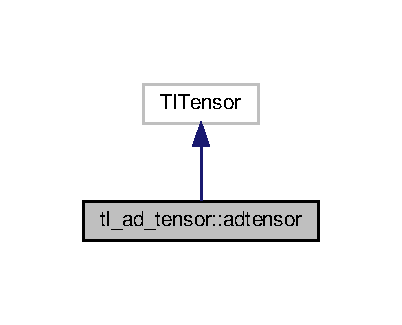
\includegraphics[width=193pt]{structtl__ad__tensor_1_1adtensor__inherit__graph}
\end{center}
\end{figure}


Collaboration diagram for tl\+\_\+ad\+\_\+tensor\+:\+:adtensor\+:\nopagebreak
\begin{figure}[H]
\begin{center}
\leavevmode
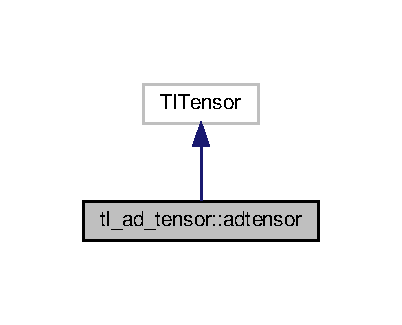
\includegraphics[width=193pt]{structtl__ad__tensor_1_1adtensor__coll__graph}
\end{center}
\end{figure}


\subsection{Detailed Description}
Tensor representation of the Adjoint tendencies. 

Definition at line 46 of file tl\+\_\+ad\+\_\+tensor.\+f90.



The documentation for this type was generated from the following file\+:\begin{DoxyCompactItemize}
\item 
tl\+\_\+ad\+\_\+tensor.\+f90\end{DoxyCompactItemize}

\hypertarget{structaotensor__def_1_1atmoctensor}{}\section{aotensor\+\_\+def\+:\+:atmoctensor Type Reference}
\label{structaotensor__def_1_1atmoctensor}\index{aotensor\+\_\+def\+::atmoctensor@{aotensor\+\_\+def\+::atmoctensor}}


Class to hold the tensor $\mathcal{T}_{i,j,k}$ representation of the tendencies.  




Collaboration diagram for aotensor\+\_\+def\+:\+:atmoctensor\+:\nopagebreak
\begin{figure}[H]
\begin{center}
\leavevmode
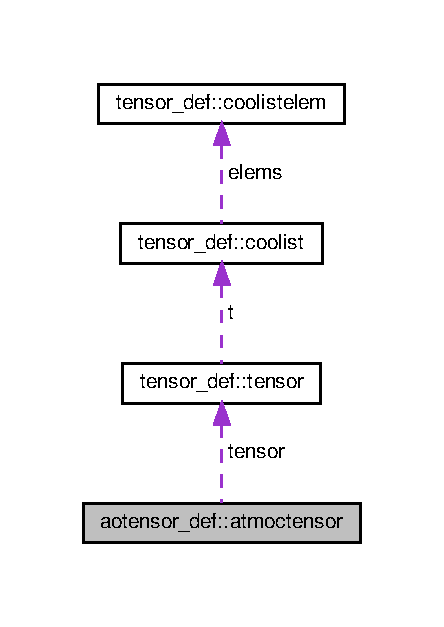
\includegraphics[width=213pt]{structaotensor__def_1_1atmoctensor__coll__graph}
\end{center}
\end{figure}
\subsection*{Public Attributes}
\begin{DoxyCompactItemize}
\item 
\mbox{\Hypertarget{structaotensor__def_1_1atmoctensor_aaf86d2b5e7f1795e126c1ef0ee8f2410}\label{structaotensor__def_1_1atmoctensor_aaf86d2b5e7f1795e126c1ef0ee8f2410}} 
type(\hyperlink{structtensor__def_1_1tensor}{tensor}) \hyperlink{structaotensor__def_1_1atmoctensor_aaf86d2b5e7f1795e126c1ef0ee8f2410}{tensor}
\begin{DoxyCompactList}\small\item\em The tensor object. \end{DoxyCompactList}\item 
\mbox{\Hypertarget{structaotensor__def_1_1atmoctensor_a5a23605208a527fa929aeb385b5481ab}\label{structaotensor__def_1_1atmoctensor_a5a23605208a527fa929aeb385b5481ab}} 
integer, dimension(\+:), allocatable \hyperlink{structaotensor__def_1_1atmoctensor_a5a23605208a527fa929aeb385b5481ab}{count\+\_\+elems}
\begin{DoxyCompactList}\small\item\em A list of the number of non-\/zero entries of the tensor component along $i$. \end{DoxyCompactList}\end{DoxyCompactItemize}


\subsection{Detailed Description}
Class to hold the tensor $\mathcal{T}_{i,j,k}$ representation of the tendencies. 

Definition at line 37 of file aotensor\+\_\+def.\+f90.



The documentation for this type was generated from the following file\+:\begin{DoxyCompactItemize}
\item 
aotensor\+\_\+def.\+f90\end{DoxyCompactItemize}

\hypertarget{structinprod__analytic_1_1atmosphereinnerproducts}{}\section{inprod\+\_\+analytic\+:\+:atmosphereinnerproducts Type Reference}
\label{structinprod__analytic_1_1atmosphereinnerproducts}\index{inprod\+\_\+analytic\+::atmosphereinnerproducts@{inprod\+\_\+analytic\+::atmosphereinnerproducts}}


Class holding the atmospheric inner products functions.  




Collaboration diagram for inprod\+\_\+analytic\+:\+:atmosphereinnerproducts\+:\nopagebreak
\begin{figure}[H]
\begin{center}
\leavevmode
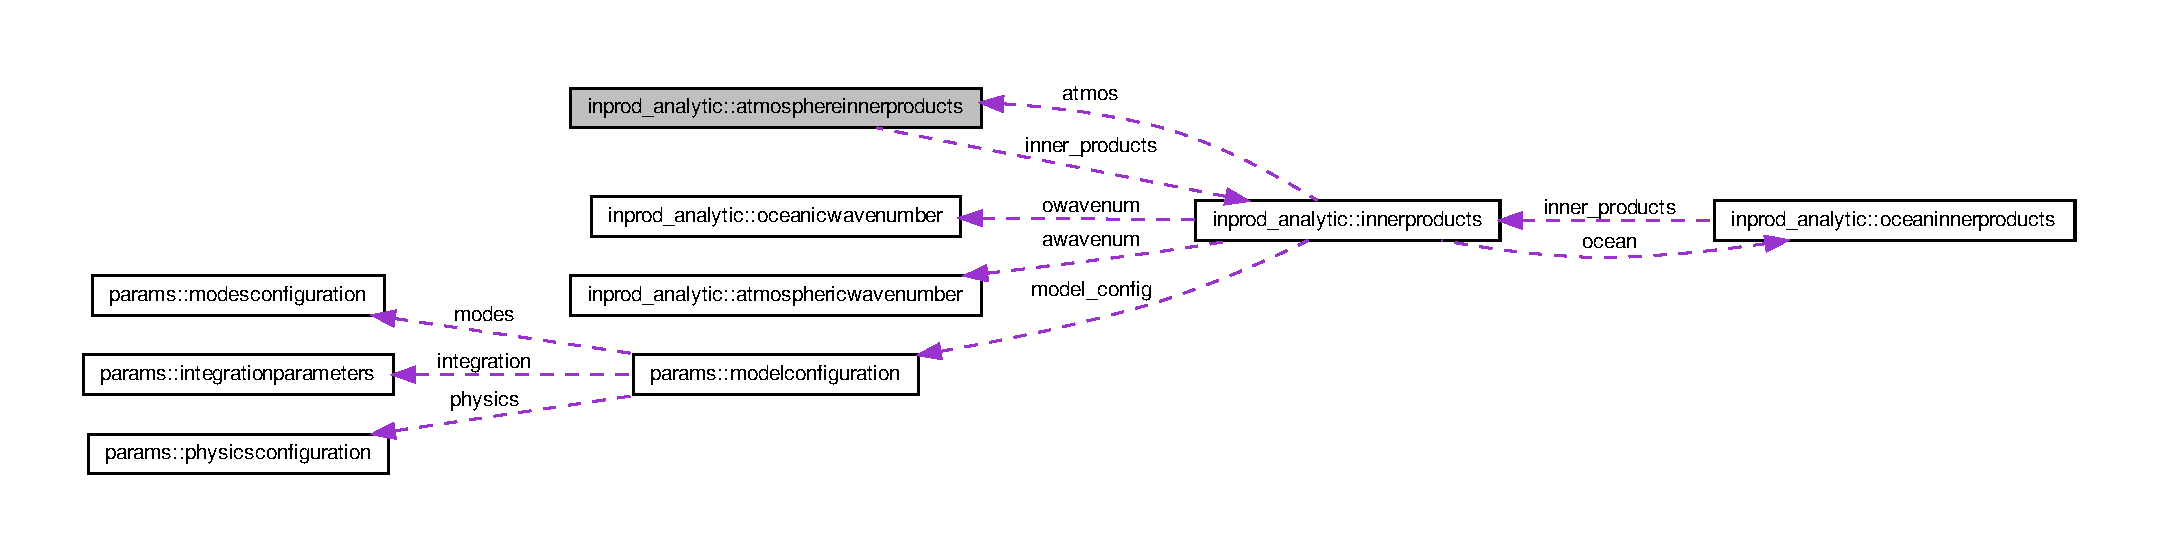
\includegraphics[width=350pt]{structinprod__analytic_1_1atmosphereinnerproducts__coll__graph}
\end{center}
\end{figure}
\subsection*{Private Member Functions}
\begin{DoxyCompactItemize}
\item 
\mbox{\Hypertarget{structinprod__analytic_1_1atmosphereinnerproducts_a5b6a547f48f8310208ae729bd1ca16d0}\label{structinprod__analytic_1_1atmosphereinnerproducts_a5b6a547f48f8310208ae729bd1ca16d0}} 
P\+R\+O\+C\+E\+D\+U\+RE \hyperlink{structinprod__analytic_1_1atmosphereinnerproducts_a5b6a547f48f8310208ae729bd1ca16d0}{a} =$>$ \hyperlink{namespaceinprod__analytic_a64153fea3801b0768d3b5122da23b324}{calculate\+\_\+a}
\begin{DoxyCompactList}\small\item\em Eigenvalues of the Laplacian (atmospheric) \end{DoxyCompactList}\item 
\mbox{\Hypertarget{structinprod__analytic_1_1atmosphereinnerproducts_ab1e9ed976ca7b9f447ffbf9105b603af}\label{structinprod__analytic_1_1atmosphereinnerproducts_ab1e9ed976ca7b9f447ffbf9105b603af}} 
P\+R\+O\+C\+E\+D\+U\+RE \hyperlink{structinprod__analytic_1_1atmosphereinnerproducts_ab1e9ed976ca7b9f447ffbf9105b603af}{b} =$>$ \hyperlink{namespaceinprod__analytic_a5608ef2b86882c7055455fbd785a8f84}{calculate\+\_\+b}
\begin{DoxyCompactList}\small\item\em Streamfunction advection terms (atmospheric) \end{DoxyCompactList}\item 
\mbox{\Hypertarget{structinprod__analytic_1_1atmosphereinnerproducts_ae06cd93cecfe277081e4037bbca88153}\label{structinprod__analytic_1_1atmosphereinnerproducts_ae06cd93cecfe277081e4037bbca88153}} 
P\+R\+O\+C\+E\+D\+U\+RE \hyperlink{structinprod__analytic_1_1atmosphereinnerproducts_ae06cd93cecfe277081e4037bbca88153}{c} =$>$ \hyperlink{namespaceinprod__analytic_aa0b310b730d6df3d09a565a09aa62a22}{calculate\+\_\+c\+\_\+atm}
\begin{DoxyCompactList}\small\item\em Beta term for the atmosphere. \end{DoxyCompactList}\item 
\mbox{\Hypertarget{structinprod__analytic_1_1atmosphereinnerproducts_aaf922f963df629246c79b7f0a5518b87}\label{structinprod__analytic_1_1atmosphereinnerproducts_aaf922f963df629246c79b7f0a5518b87}} 
P\+R\+O\+C\+E\+D\+U\+RE \hyperlink{structinprod__analytic_1_1atmosphereinnerproducts_aaf922f963df629246c79b7f0a5518b87}{d} =$>$ \hyperlink{namespaceinprod__analytic_ab270711bbfe233c1182dca363f80ec41}{calculate\+\_\+d}
\begin{DoxyCompactList}\small\item\em Forcing of the ocean on the atmosphere. \end{DoxyCompactList}\item 
\mbox{\Hypertarget{structinprod__analytic_1_1atmosphereinnerproducts_ab759d8383f4b395329f0668d04211bde}\label{structinprod__analytic_1_1atmosphereinnerproducts_ab759d8383f4b395329f0668d04211bde}} 
P\+R\+O\+C\+E\+D\+U\+RE \hyperlink{structinprod__analytic_1_1atmosphereinnerproducts_ab759d8383f4b395329f0668d04211bde}{g} =$>$ \hyperlink{namespaceinprod__analytic_ae90415e2fe9f94483e4b353afc11d245}{calculate\+\_\+g}
\begin{DoxyCompactList}\small\item\em Temperature advection terms (atmospheric) \end{DoxyCompactList}\item 
\mbox{\Hypertarget{structinprod__analytic_1_1atmosphereinnerproducts_af503c3d4a1b4234dad7d31141b5017af}\label{structinprod__analytic_1_1atmosphereinnerproducts_af503c3d4a1b4234dad7d31141b5017af}} 
P\+R\+O\+C\+E\+D\+U\+RE \hyperlink{structinprod__analytic_1_1atmosphereinnerproducts_af503c3d4a1b4234dad7d31141b5017af}{s} =$>$ \hyperlink{namespaceinprod__analytic_a3ca3072c7041b05f960b841dbcc51979}{calculate\+\_\+s}
\begin{DoxyCompactList}\small\item\em Forcing (thermal) of the ocean on the atmosphere. \end{DoxyCompactList}\end{DoxyCompactItemize}
\subsection*{Private Attributes}
\begin{DoxyCompactItemize}
\item 
\mbox{\Hypertarget{structinprod__analytic_1_1atmosphereinnerproducts_acfba9f7e96f6cb71d932ed0f2bbf24ac}\label{structinprod__analytic_1_1atmosphereinnerproducts_acfba9f7e96f6cb71d932ed0f2bbf24ac}} 
type(\hyperlink{structinprod__analytic_1_1innerproducts}{innerproducts}), pointer \hyperlink{structinprod__analytic_1_1atmosphereinnerproducts_acfba9f7e96f6cb71d932ed0f2bbf24ac}{inner\+\_\+products}
\begin{DoxyCompactList}\small\item\em Pointer to a global inner products object. \end{DoxyCompactList}\end{DoxyCompactItemize}


\subsection{Detailed Description}
Class holding the atmospheric inner products functions. 

Definition at line 51 of file inprod\+\_\+analytic.\+f90.



The documentation for this type was generated from the following file\+:\begin{DoxyCompactItemize}
\item 
inprod\+\_\+analytic.\+f90\end{DoxyCompactItemize}

\hypertarget{structinprod__analytic_1_1atmosphericwavenumber}{}\section{inprod\+\_\+analytic\+:\+:atmosphericwavenumber Type Reference}
\label{structinprod__analytic_1_1atmosphericwavenumber}\index{inprod\+\_\+analytic\+::atmosphericwavenumber@{inprod\+\_\+analytic\+::atmosphericwavenumber}}


Atmospheric bloc specification object.  




\subsection{Detailed Description}
Atmospheric bloc specification object. 

Definition at line 38 of file inprod\+\_\+analytic.\+f90.



The documentation for this type was generated from the following file\+:\begin{DoxyCompactItemize}
\item 
inprod\+\_\+analytic.\+f90\end{DoxyCompactItemize}

\hypertarget{interfaceintegrator__def_1_1clean__int}{}\section{integrator\+\_\+def\+:\+:clean\+\_\+int Interface Reference}
\label{interfaceintegrator__def_1_1clean__int}\index{integrator\+\_\+def\+::clean\+\_\+int@{integrator\+\_\+def\+::clean\+\_\+int}}


Abstract interface for the procedure to clean the integrator objects.  




\subsection{Detailed Description}
Abstract interface for the procedure to clean the integrator objects. 


\begin{DoxyParams}[1]{Parameters}
\mbox{\tt in,out}  & {\em integr} & Integrator object to clean. \\
\hline
\end{DoxyParams}


Definition at line 62 of file integrator\+\_\+def.\+f90.



The documentation for this interface was generated from the following file\+:\begin{DoxyCompactItemize}
\item 
integrator\+\_\+def.\+f90\end{DoxyCompactItemize}

\hypertarget{structtensor__def_1_1coolist}{}\section{tensor\+\_\+def\+:\+:coolist Type Reference}
\label{structtensor__def_1_1coolist}\index{tensor\+\_\+def\+::coolist@{tensor\+\_\+def\+::coolist}}


Coordinate list. Type used to represent the sparse tensor.  




Collaboration diagram for tensor\+\_\+def\+:\+:coolist\+:\nopagebreak
\begin{figure}[H]
\begin{center}
\leavevmode
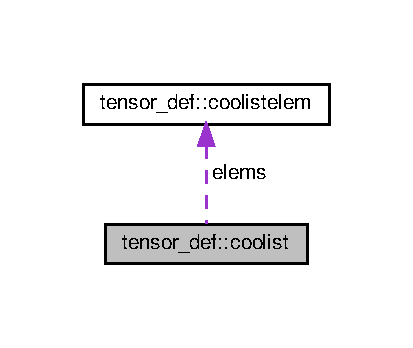
\includegraphics[width=198pt]{structtensor__def_1_1coolist__coll__graph}
\end{center}
\end{figure}
\subsection*{Private Attributes}
\begin{DoxyCompactItemize}
\item 
\mbox{\Hypertarget{structtensor__def_1_1coolist_a41e00da023c2c01ce5010940170c24b6}\label{structtensor__def_1_1coolist_a41e00da023c2c01ce5010940170c24b6}} 
type(\hyperlink{structtensor__def_1_1coolistelem}{coolistelem}), dimension(\+:), allocatable \hyperlink{structtensor__def_1_1coolist_a41e00da023c2c01ce5010940170c24b6}{elems}
\begin{DoxyCompactList}\small\item\em Lists of elements tensor\+\_\+def\+::coolist\+\_\+elem. \end{DoxyCompactList}\item 
\mbox{\Hypertarget{structtensor__def_1_1coolist_acbdf5af7f599640405c1d194c87c07fd}\label{structtensor__def_1_1coolist_acbdf5af7f599640405c1d194c87c07fd}} 
integer \hyperlink{structtensor__def_1_1coolist_acbdf5af7f599640405c1d194c87c07fd}{nelems} = 0
\begin{DoxyCompactList}\small\item\em Number of elements in the list. \end{DoxyCompactList}\end{DoxyCompactItemize}


\subsection{Detailed Description}
Coordinate list. Type used to represent the sparse tensor. 

Definition at line 30 of file tensor\+\_\+def.\+f90.



The documentation for this type was generated from the following file\+:\begin{DoxyCompactItemize}
\item 
tensor\+\_\+def.\+f90\end{DoxyCompactItemize}

\hypertarget{structtensor__def_1_1coolistelem}{}\section{tensor\+\_\+def\+:\+:coolistelem Type Reference}
\label{structtensor__def_1_1coolistelem}\index{tensor\+\_\+def\+::coolistelem@{tensor\+\_\+def\+::coolistelem}}


Coordinate list element type. Elementary elements of the sparse tensors.  


\subsection*{Private Attributes}
\begin{DoxyCompactItemize}
\item 
\mbox{\Hypertarget{structtensor__def_1_1coolistelem_a72243a3a466371a2d71ba4a9da505a34}\label{structtensor__def_1_1coolistelem_a72243a3a466371a2d71ba4a9da505a34}} 
integer \hyperlink{structtensor__def_1_1coolistelem_a72243a3a466371a2d71ba4a9da505a34}{j}
\begin{DoxyCompactList}\small\item\em Index $j$ of the element. \end{DoxyCompactList}\item 
\mbox{\Hypertarget{structtensor__def_1_1coolistelem_a644211f265e9a4fc712f3bc7d1362712}\label{structtensor__def_1_1coolistelem_a644211f265e9a4fc712f3bc7d1362712}} 
integer \hyperlink{structtensor__def_1_1coolistelem_a644211f265e9a4fc712f3bc7d1362712}{k}
\begin{DoxyCompactList}\small\item\em Index $k$ of the element. \end{DoxyCompactList}\item 
\mbox{\Hypertarget{structtensor__def_1_1coolistelem_a67b9432a8f7621a51129b48e3749bdf0}\label{structtensor__def_1_1coolistelem_a67b9432a8f7621a51129b48e3749bdf0}} 
real(kind=8) \hyperlink{structtensor__def_1_1coolistelem_a67b9432a8f7621a51129b48e3749bdf0}{v}
\begin{DoxyCompactList}\small\item\em Value of the element. \end{DoxyCompactList}\end{DoxyCompactItemize}


\subsection{Detailed Description}
Coordinate list element type. Elementary elements of the sparse tensors. 

Definition at line 23 of file tensor\+\_\+def.\+f90.



The documentation for this type was generated from the following file\+:\begin{DoxyCompactItemize}
\item 
tensor\+\_\+def.\+f90\end{DoxyCompactItemize}

\hypertarget{interfaceintegrator__def_1_1init__int}{}\section{integrator\+\_\+def\+:\+:init\+\_\+int Interface Reference}
\label{interfaceintegrator__def_1_1init__int}\index{integrator\+\_\+def\+::init\+\_\+int@{integrator\+\_\+def\+::init\+\_\+int}}


Abstract interface for the procedures initializing the integrator objects.  




\subsection{Detailed Description}
Abstract interface for the procedures initializing the integrator objects. 


\begin{DoxyParams}[1]{Parameters}
\mbox{\tt in,out}  & {\em integr} & Integrator object to initialize. \\
\hline
\mbox{\tt in}  & {\em imodel} & Model object to initialize the integrator with. \\
\hline
\end{DoxyParams}


Definition at line 37 of file integrator\+\_\+def.\+f90.



The documentation for this interface was generated from the following file\+:\begin{DoxyCompactItemize}
\item 
integrator\+\_\+def.\+f90\end{DoxyCompactItemize}

\hypertarget{structinprod__analytic_1_1innerproducts}{}\section{inprod\+\_\+analytic\+:\+:innerproducts Type Reference}
\label{structinprod__analytic_1_1innerproducts}\index{inprod\+\_\+analytic\+::innerproducts@{inprod\+\_\+analytic\+::innerproducts}}


Global class for the inner products. Contains also the modes informations.  




Collaboration diagram for inprod\+\_\+analytic\+:\+:innerproducts\+:\nopagebreak
\begin{figure}[H]
\begin{center}
\leavevmode
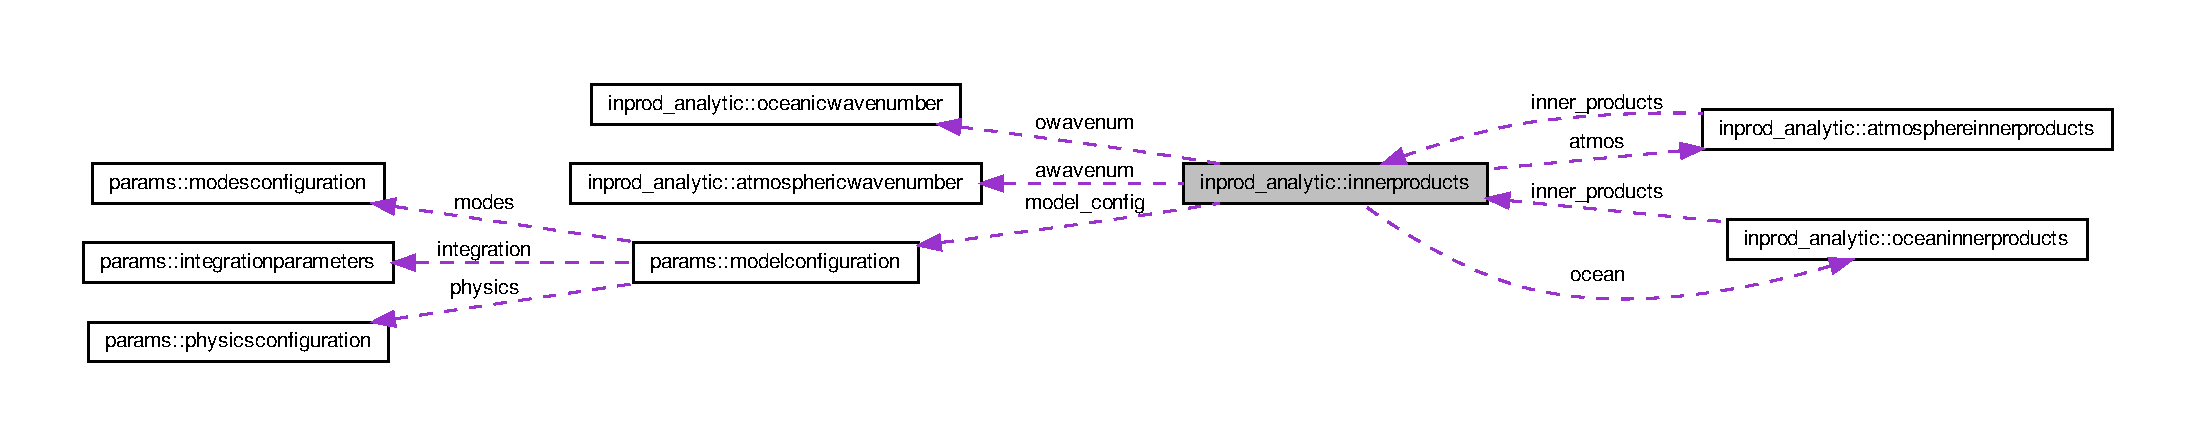
\includegraphics[width=350pt]{structinprod__analytic_1_1innerproducts__coll__graph}
\end{center}
\end{figure}
\subsection*{Public Member Functions}
\begin{DoxyCompactItemize}
\item 
\mbox{\Hypertarget{structinprod__analytic_1_1innerproducts_a76f38356e38405a715ad3c8cff7a6781}\label{structinprod__analytic_1_1innerproducts_a76f38356e38405a715ad3c8cff7a6781}} 
P\+R\+O\+C\+E\+D\+U\+RE \hyperlink{structinprod__analytic_1_1innerproducts_a76f38356e38405a715ad3c8cff7a6781}{init} =$>$ \hyperlink{namespaceinprod__analytic_ad2e5c28272f877bf96af8ee821004386}{init\+\_\+inner\+\_\+products}
\begin{DoxyCompactList}\small\item\em Procedure to initialize the inner products functions based on the modes configuration. \end{DoxyCompactList}\item 
\mbox{\Hypertarget{structinprod__analytic_1_1innerproducts_a5ea60d33169a70443f5581108a0f5100}\label{structinprod__analytic_1_1innerproducts_a5ea60d33169a70443f5581108a0f5100}} 
P\+R\+O\+C\+E\+D\+U\+RE \hyperlink{structinprod__analytic_1_1innerproducts_a5ea60d33169a70443f5581108a0f5100}{clean} =$>$ \hyperlink{namespaceinprod__analytic_a1319e98f839daff8d840469929c349fb}{delete\+\_\+inner\+\_\+products}
\begin{DoxyCompactList}\small\item\em Procedure to clean the inner products object. \end{DoxyCompactList}\end{DoxyCompactItemize}
\subsection*{Public Attributes}
\begin{DoxyCompactItemize}
\item 
\mbox{\Hypertarget{structinprod__analytic_1_1innerproducts_a52339677473eea2827db0a0c5d160b37}\label{structinprod__analytic_1_1innerproducts_a52339677473eea2827db0a0c5d160b37}} 
type(\hyperlink{structparams_1_1modelconfiguration}{modelconfiguration}), pointer \hyperlink{structinprod__analytic_1_1innerproducts_a52339677473eea2827db0a0c5d160b37}{model\+\_\+config}
\begin{DoxyCompactList}\small\item\em Pointer to a model configuration object. \end{DoxyCompactList}\item 
\mbox{\Hypertarget{structinprod__analytic_1_1innerproducts_a030638396f82eb8c2419789708995d2d}\label{structinprod__analytic_1_1innerproducts_a030638396f82eb8c2419789708995d2d}} 
type(\hyperlink{structinprod__analytic_1_1atmosphericwavenumber}{atmosphericwavenumber}), dimension(\+:), allocatable, public \hyperlink{structinprod__analytic_1_1innerproducts_a030638396f82eb8c2419789708995d2d}{awavenum}
\begin{DoxyCompactList}\small\item\em Atmospheric blocs specification. \end{DoxyCompactList}\item 
\mbox{\Hypertarget{structinprod__analytic_1_1innerproducts_a7cd1a769aa1468eafce276b25bde03ee}\label{structinprod__analytic_1_1innerproducts_a7cd1a769aa1468eafce276b25bde03ee}} 
type(\hyperlink{structinprod__analytic_1_1oceanicwavenumber}{oceanicwavenumber}), dimension(\+:), allocatable, public \hyperlink{structinprod__analytic_1_1innerproducts_a7cd1a769aa1468eafce276b25bde03ee}{owavenum}
\begin{DoxyCompactList}\small\item\em Oceanic blocs specification. \end{DoxyCompactList}\item 
\mbox{\Hypertarget{structinprod__analytic_1_1innerproducts_a812c82c549eb1a53e3259844bb6766b4}\label{structinprod__analytic_1_1innerproducts_a812c82c549eb1a53e3259844bb6766b4}} 
type(\hyperlink{structinprod__analytic_1_1atmosphereinnerproducts}{atmosphereinnerproducts}), public \hyperlink{structinprod__analytic_1_1innerproducts_a812c82c549eb1a53e3259844bb6766b4}{atmos}
\begin{DoxyCompactList}\small\item\em Atmospheric tensors. \end{DoxyCompactList}\item 
\mbox{\Hypertarget{structinprod__analytic_1_1innerproducts_a349a38f433c62a09f3f4cd9720bdea14}\label{structinprod__analytic_1_1innerproducts_a349a38f433c62a09f3f4cd9720bdea14}} 
type(\hyperlink{structinprod__analytic_1_1oceaninnerproducts}{oceaninnerproducts}), public \hyperlink{structinprod__analytic_1_1innerproducts_a349a38f433c62a09f3f4cd9720bdea14}{ocean}
\begin{DoxyCompactList}\small\item\em Oceanic tensors. \end{DoxyCompactList}\end{DoxyCompactItemize}


\subsection{Detailed Description}
Global class for the inner products. Contains also the modes informations. 

Definition at line 75 of file inprod\+\_\+analytic.\+f90.



The documentation for this type was generated from the following file\+:\begin{DoxyCompactItemize}
\item 
inprod\+\_\+analytic.\+f90\end{DoxyCompactItemize}

\hypertarget{structparams_1_1integrationparameters}{}\section{params\+:\+:integrationparameters Type Reference}
\label{structparams_1_1integrationparameters}\index{params\+::integrationparameters@{params\+::integrationparameters}}


The subclass containing the integration parameters.  


\subsection*{Public Attributes}
\begin{DoxyCompactItemize}
\item 
\mbox{\Hypertarget{structparams_1_1integrationparameters_a73a172332bf1bcd0cf80563956500dde}\label{structparams_1_1integrationparameters_a73a172332bf1bcd0cf80563956500dde}} 
real(kind=8) \hyperlink{structparams_1_1integrationparameters_a73a172332bf1bcd0cf80563956500dde}{t\+\_\+trans}
\begin{DoxyCompactList}\small\item\em Transient time period. \end{DoxyCompactList}\item 
\mbox{\Hypertarget{structparams_1_1integrationparameters_a85f473fb6ea786e419dd376d4f8980fd}\label{structparams_1_1integrationparameters_a85f473fb6ea786e419dd376d4f8980fd}} 
real(kind=8) \hyperlink{structparams_1_1integrationparameters_a85f473fb6ea786e419dd376d4f8980fd}{t\+\_\+run}
\begin{DoxyCompactList}\small\item\em Effective intergration time (length of the generated trajectory) \end{DoxyCompactList}\item 
\mbox{\Hypertarget{structparams_1_1integrationparameters_aabc133bb728aff702de1f9ec824d4b41}\label{structparams_1_1integrationparameters_aabc133bb728aff702de1f9ec824d4b41}} 
real(kind=8) \hyperlink{structparams_1_1integrationparameters_aabc133bb728aff702de1f9ec824d4b41}{dt}
\begin{DoxyCompactList}\small\item\em Integration time step. \end{DoxyCompactList}\item 
\mbox{\Hypertarget{structparams_1_1integrationparameters_a33a3ac774f065b62c2aa2e44da39537a}\label{structparams_1_1integrationparameters_a33a3ac774f065b62c2aa2e44da39537a}} 
real(kind=8) \hyperlink{structparams_1_1integrationparameters_a33a3ac774f065b62c2aa2e44da39537a}{tw}
\begin{DoxyCompactList}\small\item\em Write all variables every tw time units. \end{DoxyCompactList}\item 
\mbox{\Hypertarget{structparams_1_1integrationparameters_a0b652b1ecf7abd3d54091d885095d409}\label{structparams_1_1integrationparameters_a0b652b1ecf7abd3d54091d885095d409}} 
real(kind=8) \hyperlink{structparams_1_1integrationparameters_a0b652b1ecf7abd3d54091d885095d409}{tw\+\_\+snap}
\begin{DoxyCompactList}\small\item\em Write a snapshot every tw\+\_\+snap time units. \end{DoxyCompactList}\item 
\mbox{\Hypertarget{structparams_1_1integrationparameters_a04886fca9e3ccef570ea098350846d44}\label{structparams_1_1integrationparameters_a04886fca9e3ccef570ea098350846d44}} 
logical \hyperlink{structparams_1_1integrationparameters_a04886fca9e3ccef570ea098350846d44}{writeout}
\begin{DoxyCompactList}\small\item\em Write to file boolean. \end{DoxyCompactList}\end{DoxyCompactItemize}


\subsection{Detailed Description}
The subclass containing the integration parameters. 

Definition at line 79 of file params.\+f90.



The documentation for this type was generated from the following file\+:\begin{DoxyCompactItemize}
\item 
params.\+f90\end{DoxyCompactItemize}

\hypertarget{structintegrator__def_1_1integrator}{}\section{integrator\+\_\+def\+:\+:integrator Type Reference}
\label{structintegrator__def_1_1integrator}\index{integrator\+\_\+def\+::integrator@{integrator\+\_\+def\+::integrator}}


Base class to be subclassed to create a new integrator.  




Collaboration diagram for integrator\+\_\+def\+:\+:integrator\+:\nopagebreak
\begin{figure}[H]
\begin{center}
\leavevmode
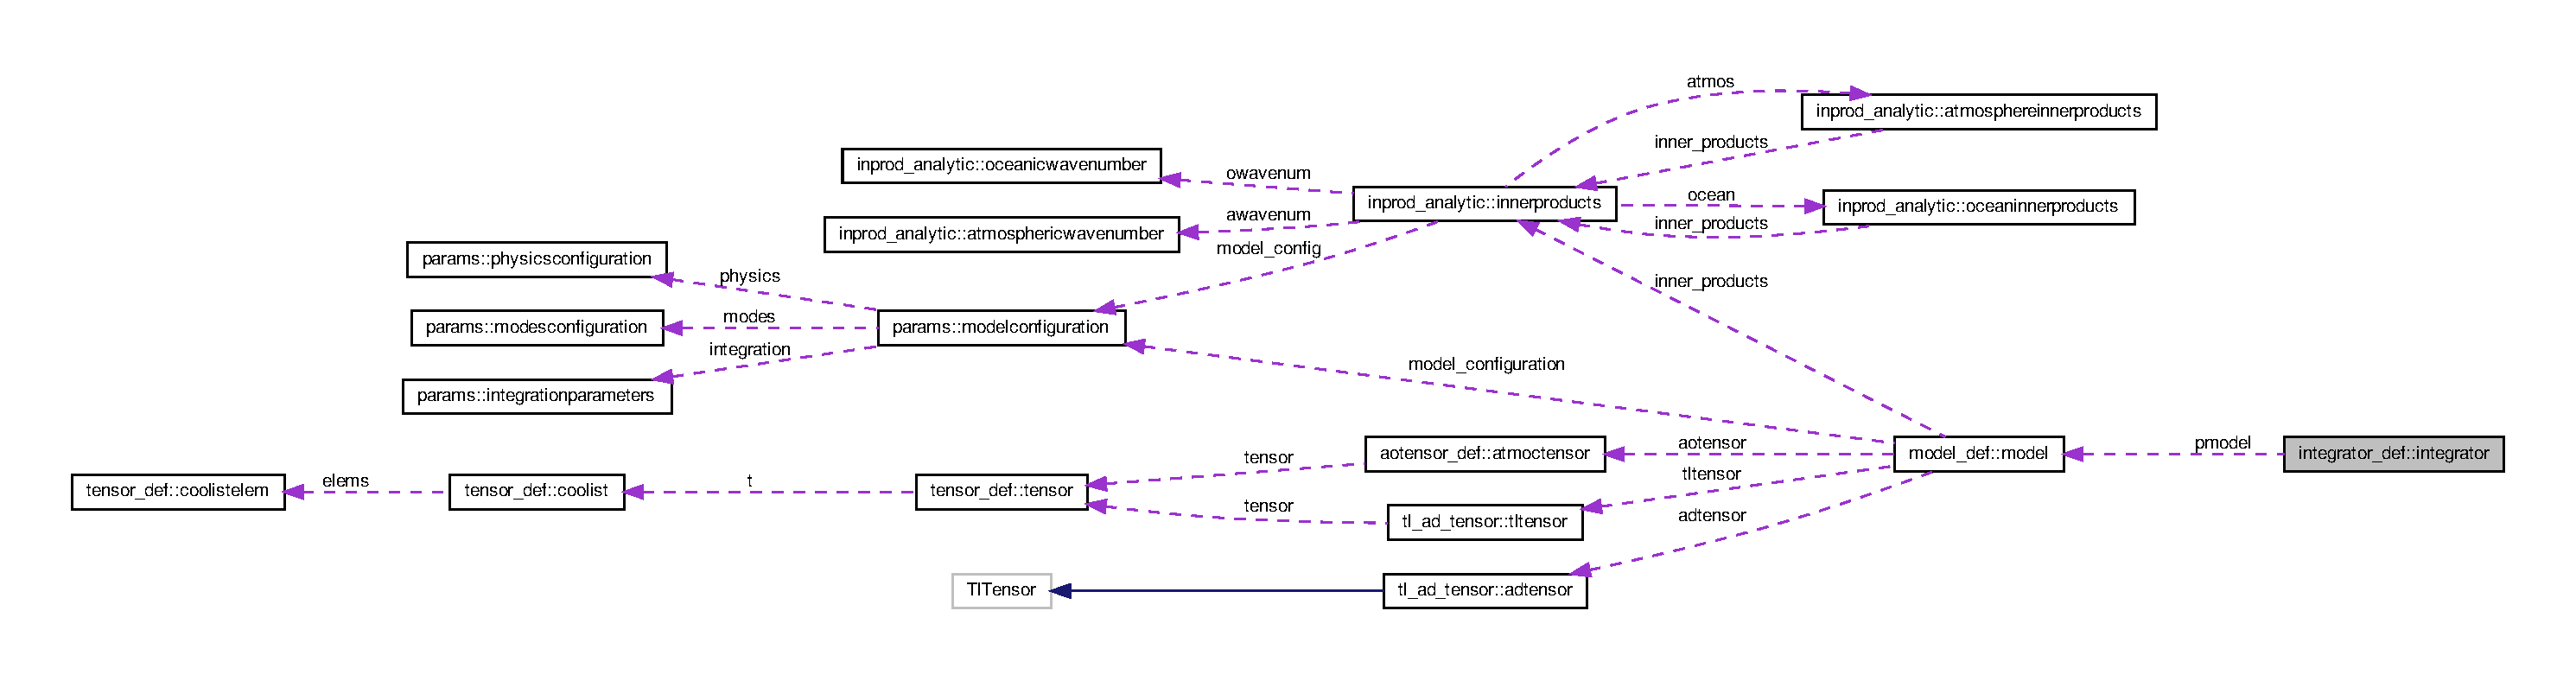
\includegraphics[width=350pt]{structintegrator__def_1_1integrator__coll__graph}
\end{center}
\end{figure}
\subsection*{Public Attributes}
\begin{DoxyCompactItemize}
\item 
\mbox{\Hypertarget{structintegrator__def_1_1integrator_a1d261286cba5b917c64b348f5b903e64}\label{structintegrator__def_1_1integrator_a1d261286cba5b917c64b348f5b903e64}} 
type(\hyperlink{structmodel__def_1_1model}{model}), pointer \hyperlink{structintegrator__def_1_1integrator_a1d261286cba5b917c64b348f5b903e64}{pmodel}
\begin{DoxyCompactList}\small\item\em A pointer to the model to integrate. \end{DoxyCompactList}\item 
\mbox{\Hypertarget{structintegrator__def_1_1integrator_a086de7ff5ed4454ad5804312970b516c}\label{structintegrator__def_1_1integrator_a086de7ff5ed4454ad5804312970b516c}} 
real(kind=8), pointer \hyperlink{structintegrator__def_1_1integrator_a086de7ff5ed4454ad5804312970b516c}{dt}
\begin{DoxyCompactList}\small\item\em Time step of the integrator. \end{DoxyCompactList}\item 
\mbox{\Hypertarget{structintegrator__def_1_1integrator_a3e374d290b3754d2079de91068314f2e}\label{structintegrator__def_1_1integrator_a3e374d290b3754d2079de91068314f2e}} 
integer, pointer \hyperlink{structintegrator__def_1_1integrator_a3e374d290b3754d2079de91068314f2e}{ndim}
\begin{DoxyCompactList}\small\item\em Dimension of the phase space of the model to integrate. \end{DoxyCompactList}\end{DoxyCompactItemize}


\subsection{Detailed Description}
Base class to be subclassed to create a new integrator. 

Definition at line 23 of file integrator\+\_\+def.\+f90.



The documentation for this type was generated from the following file\+:\begin{DoxyCompactItemize}
\item 
integrator\+\_\+def.\+f90\end{DoxyCompactItemize}

\hypertarget{structmodel__def_1_1model}{}\section{model\+\_\+def\+:\+:model Type Reference}
\label{structmodel__def_1_1model}\index{model\+\_\+def\+::model@{model\+\_\+def\+::model}}


Class to hold the components of a model version.  




Collaboration diagram for model\+\_\+def\+:\+:model\+:\nopagebreak
\begin{figure}[H]
\begin{center}
\leavevmode
\includegraphics[width=350pt]{structmodel__def_1_1model__coll__graph}
\end{center}
\end{figure}
\subsection*{Public Attributes}
\begin{DoxyCompactItemize}
\item 
\mbox{\Hypertarget{structmodel__def_1_1model_a51357fc425ffbcac7379506674ab160a}\label{structmodel__def_1_1model_a51357fc425ffbcac7379506674ab160a}} 
type(\hyperlink{structparams_1_1modelconfiguration}{modelconfiguration}) \hyperlink{structmodel__def_1_1model_a51357fc425ffbcac7379506674ab160a}{model\+\_\+configuration}
\begin{DoxyCompactList}\small\item\em Model configuration object of the model. \end{DoxyCompactList}\item 
\mbox{\Hypertarget{structmodel__def_1_1model_adf914bba30b77b03601cfb3e7415a272}\label{structmodel__def_1_1model_adf914bba30b77b03601cfb3e7415a272}} 
type(\hyperlink{structinprod__analytic_1_1innerproducts}{innerproducts}) \hyperlink{structmodel__def_1_1model_adf914bba30b77b03601cfb3e7415a272}{inner\+\_\+products}
\begin{DoxyCompactList}\small\item\em Inner products object of the model. \end{DoxyCompactList}\item 
\mbox{\Hypertarget{structmodel__def_1_1model_aafe9a0c31d2c25378a9e08a3dab66ba5}\label{structmodel__def_1_1model_aafe9a0c31d2c25378a9e08a3dab66ba5}} 
type(\hyperlink{structaotensor__def_1_1atmoctensor}{atmoctensor}) \hyperlink{structmodel__def_1_1model_aafe9a0c31d2c25378a9e08a3dab66ba5}{aotensor}
\begin{DoxyCompactList}\small\item\em Atmosphere-\/\+Ocean tendencies tensor of the model. \end{DoxyCompactList}\item 
\mbox{\Hypertarget{structmodel__def_1_1model_ad1aef0b2a70dd7921c07d8d929513c23}\label{structmodel__def_1_1model_ad1aef0b2a70dd7921c07d8d929513c23}} 
type(\hyperlink{structtl__ad__tensor_1_1tltensor}{tltensor}) \hyperlink{structmodel__def_1_1model_ad1aef0b2a70dd7921c07d8d929513c23}{tltensor}
\begin{DoxyCompactList}\small\item\em Tangent linear model tendencies. \end{DoxyCompactList}\item 
\mbox{\Hypertarget{structmodel__def_1_1model_a5fd98607a716156493328f547110c4fb}\label{structmodel__def_1_1model_a5fd98607a716156493328f547110c4fb}} 
type(\hyperlink{structtl__ad__tensor_1_1adtensor}{adtensor}) \hyperlink{structmodel__def_1_1model_a5fd98607a716156493328f547110c4fb}{adtensor}
\begin{DoxyCompactList}\small\item\em Adjoint model tendencies. \end{DoxyCompactList}\item 
\mbox{\Hypertarget{structmodel__def_1_1model_a7d00fa265bddc896253a230a906f02e5}\label{structmodel__def_1_1model_a7d00fa265bddc896253a230a906f02e5}} 
integer, pointer \hyperlink{structmodel__def_1_1model_a7d00fa265bddc896253a230a906f02e5}{ndim}
\begin{DoxyCompactList}\small\item\em Dimension of the phase space of the model to integrate. \end{DoxyCompactList}\end{DoxyCompactItemize}


\subsection{Detailed Description}
Class to hold the components of a model version. 

Definition at line 25 of file model\+\_\+def.\+f90.



The documentation for this type was generated from the following file\+:\begin{DoxyCompactItemize}
\item 
model\+\_\+def.\+f90\end{DoxyCompactItemize}

\hypertarget{structparams_1_1modelconfiguration}{}\section{params\+:\+:modelconfiguration Type Reference}
\label{structparams_1_1modelconfiguration}\index{params\+::modelconfiguration@{params\+::modelconfiguration}}


The general class holding the model configuration.  




Collaboration diagram for params\+:\+:modelconfiguration\+:\nopagebreak
\begin{figure}[H]
\begin{center}
\leavevmode
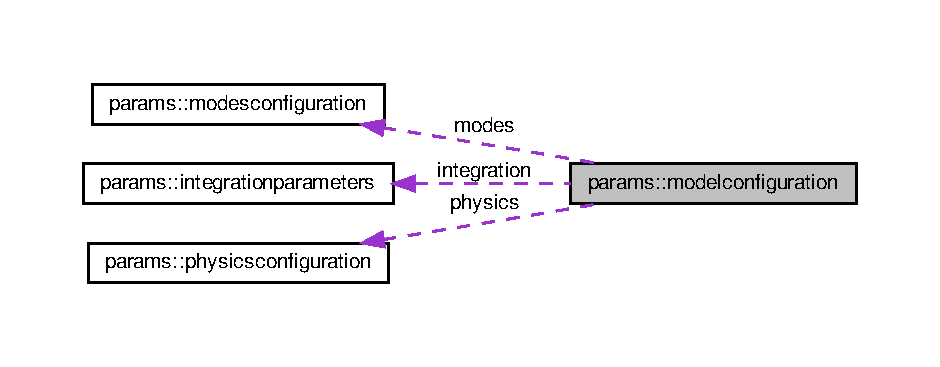
\includegraphics[width=350pt]{structparams_1_1modelconfiguration__coll__graph}
\end{center}
\end{figure}


\subsection{Detailed Description}
The general class holding the model configuration. 

Definition at line 107 of file params.\+f90.



The documentation for this type was generated from the following file\+:\begin{DoxyCompactItemize}
\item 
params.\+f90\end{DoxyCompactItemize}

\hypertarget{structparams_1_1modesconfiguration}{}\section{params\+:\+:modesconfiguration Type Reference}
\label{structparams_1_1modesconfiguration}\index{params\+::modesconfiguration@{params\+::modesconfiguration}}


The subclass containing the modes parameters.  


\subsection*{Public Attributes}
\begin{DoxyCompactItemize}
\item 
\mbox{\Hypertarget{structparams_1_1modesconfiguration_a69a0793ecee9913a43b12001b3bd96ba}\label{structparams_1_1modesconfiguration_a69a0793ecee9913a43b12001b3bd96ba}} 
integer \hyperlink{structparams_1_1modesconfiguration_a69a0793ecee9913a43b12001b3bd96ba}{nboc}
\begin{DoxyCompactList}\small\item\em Number of atmospheric blocks. \end{DoxyCompactList}\item 
\mbox{\Hypertarget{structparams_1_1modesconfiguration_a26c0b1a58aa2ac7a17b59cf4ec0a1be8}\label{structparams_1_1modesconfiguration_a26c0b1a58aa2ac7a17b59cf4ec0a1be8}} 
integer \hyperlink{structparams_1_1modesconfiguration_a26c0b1a58aa2ac7a17b59cf4ec0a1be8}{nbatm}
\begin{DoxyCompactList}\small\item\em Number of oceanic blocks. \end{DoxyCompactList}\item 
\mbox{\Hypertarget{structparams_1_1modesconfiguration_a10bce57d0b89eaf60320cec21bb75857}\label{structparams_1_1modesconfiguration_a10bce57d0b89eaf60320cec21bb75857}} 
integer, dimension(\+:,\+:), allocatable \hyperlink{structparams_1_1modesconfiguration_a10bce57d0b89eaf60320cec21bb75857}{oms}
\begin{DoxyCompactList}\small\item\em Ocean mode selection array. \end{DoxyCompactList}\item 
\mbox{\Hypertarget{structparams_1_1modesconfiguration_aa011e841259b6bfb4fd691fbc31154b3}\label{structparams_1_1modesconfiguration_aa011e841259b6bfb4fd691fbc31154b3}} 
integer, dimension(\+:,\+:), allocatable \hyperlink{structparams_1_1modesconfiguration_aa011e841259b6bfb4fd691fbc31154b3}{ams}
\begin{DoxyCompactList}\small\item\em Atmospheric mode selection array. \end{DoxyCompactList}\item 
\mbox{\Hypertarget{structparams_1_1modesconfiguration_a7ede74e1e6b6d7cda3dd09a02797a884}\label{structparams_1_1modesconfiguration_a7ede74e1e6b6d7cda3dd09a02797a884}} 
integer \hyperlink{structparams_1_1modesconfiguration_a7ede74e1e6b6d7cda3dd09a02797a884}{natm} =0
\begin{DoxyCompactList}\small\item\em Number of atmospheric basis functions. \end{DoxyCompactList}\item 
\mbox{\Hypertarget{structparams_1_1modesconfiguration_a1e4bfd9c3ab523dcb6b8f7547cc4e8ca}\label{structparams_1_1modesconfiguration_a1e4bfd9c3ab523dcb6b8f7547cc4e8ca}} 
integer \hyperlink{structparams_1_1modesconfiguration_a1e4bfd9c3ab523dcb6b8f7547cc4e8ca}{noc} =0
\begin{DoxyCompactList}\small\item\em Number of oceanic basis functions. \end{DoxyCompactList}\item 
\mbox{\Hypertarget{structparams_1_1modesconfiguration_aadba4b01a2ee12635e80e3ef183f8b51}\label{structparams_1_1modesconfiguration_aadba4b01a2ee12635e80e3ef183f8b51}} 
integer \hyperlink{structparams_1_1modesconfiguration_aadba4b01a2ee12635e80e3ef183f8b51}{ndim}
\begin{DoxyCompactList}\small\item\em Number of variables (dimension of the model) \end{DoxyCompactList}\end{DoxyCompactItemize}


\subsection{Detailed Description}
The subclass containing the modes parameters. 

Definition at line 92 of file params.\+f90.



The documentation for this type was generated from the following file\+:\begin{DoxyCompactItemize}
\item 
params.\+f90\end{DoxyCompactItemize}

\hypertarget{structinprod__analytic_1_1oceanicwavenumber}{}\section{inprod\+\_\+analytic\+:\+:oceanicwavenumber Type Reference}
\label{structinprod__analytic_1_1oceanicwavenumber}\index{inprod\+\_\+analytic\+::oceanicwavenumber@{inprod\+\_\+analytic\+::oceanicwavenumber}}


Oceanic bloc specification object.  




\subsection{Detailed Description}
Oceanic bloc specification object. 

Definition at line 45 of file inprod\+\_\+analytic.\+f90.



The documentation for this type was generated from the following file\+:\begin{DoxyCompactItemize}
\item 
inprod\+\_\+analytic.\+f90\end{DoxyCompactItemize}

\hypertarget{structinprod__analytic_1_1oceaninnerproducts}{}\section{inprod\+\_\+analytic\+:\+:oceaninnerproducts Type Reference}
\label{structinprod__analytic_1_1oceaninnerproducts}\index{inprod\+\_\+analytic\+::oceaninnerproducts@{inprod\+\_\+analytic\+::oceaninnerproducts}}


Class holding the oceanic inner products functions.  




Collaboration diagram for inprod\+\_\+analytic\+:\+:oceaninnerproducts\+:\nopagebreak
\begin{figure}[H]
\begin{center}
\leavevmode
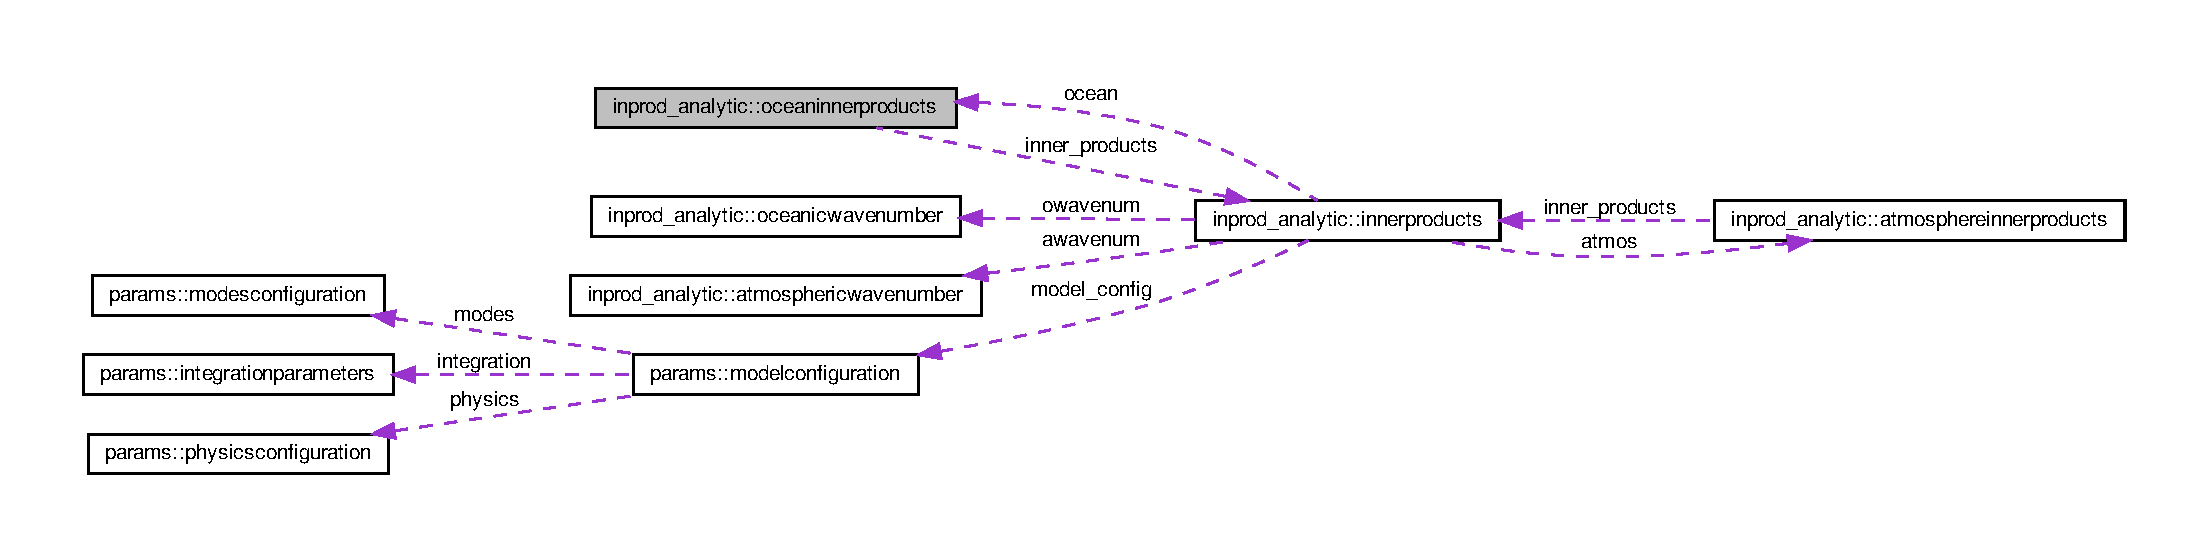
\includegraphics[width=350pt]{structinprod__analytic_1_1oceaninnerproducts__coll__graph}
\end{center}
\end{figure}
\subsection*{Private Member Functions}
\begin{DoxyCompactItemize}
\item 
\mbox{\Hypertarget{structinprod__analytic_1_1oceaninnerproducts_a9307f24bb98418072a02fe1316dfbe93}\label{structinprod__analytic_1_1oceaninnerproducts_a9307f24bb98418072a02fe1316dfbe93}} 
P\+R\+O\+C\+E\+D\+U\+RE \hyperlink{structinprod__analytic_1_1oceaninnerproducts_a9307f24bb98418072a02fe1316dfbe93}{k} =$>$ calculate\+\_\+K
\begin{DoxyCompactList}\small\item\em Forcing of the atmosphere on the ocean. \end{DoxyCompactList}\item 
\mbox{\Hypertarget{structinprod__analytic_1_1oceaninnerproducts_aaf4ddf2fbb55e5f1a6993df01882f124}\label{structinprod__analytic_1_1oceaninnerproducts_aaf4ddf2fbb55e5f1a6993df01882f124}} 
P\+R\+O\+C\+E\+D\+U\+RE \hyperlink{structinprod__analytic_1_1oceaninnerproducts_aaf4ddf2fbb55e5f1a6993df01882f124}{m} =$>$ calculate\+\_\+M
\begin{DoxyCompactList}\small\item\em Forcing of the ocean fields on the ocean. \end{DoxyCompactList}\item 
\mbox{\Hypertarget{structinprod__analytic_1_1oceaninnerproducts_accb0af974da31afbc92402f3bc5ba3f1}\label{structinprod__analytic_1_1oceaninnerproducts_accb0af974da31afbc92402f3bc5ba3f1}} 
P\+R\+O\+C\+E\+D\+U\+RE \hyperlink{structinprod__analytic_1_1oceaninnerproducts_accb0af974da31afbc92402f3bc5ba3f1}{c} =$>$ calculate\+\_\+\+C\+\_\+oc
\begin{DoxyCompactList}\small\item\em Streamfunction advection terms (oceanic) \end{DoxyCompactList}\item 
\mbox{\Hypertarget{structinprod__analytic_1_1oceaninnerproducts_ad98419788cc39ab5d6408d9a56360ebb}\label{structinprod__analytic_1_1oceaninnerproducts_ad98419788cc39ab5d6408d9a56360ebb}} 
P\+R\+O\+C\+E\+D\+U\+RE \hyperlink{structinprod__analytic_1_1oceaninnerproducts_ad98419788cc39ab5d6408d9a56360ebb}{n} =$>$ calculate\+\_\+N
\begin{DoxyCompactList}\small\item\em Beta term for the ocean. \end{DoxyCompactList}\item 
\mbox{\Hypertarget{structinprod__analytic_1_1oceaninnerproducts_acf470fb66c8ac2447a5d990e42bf80e3}\label{structinprod__analytic_1_1oceaninnerproducts_acf470fb66c8ac2447a5d990e42bf80e3}} 
P\+R\+O\+C\+E\+D\+U\+RE \hyperlink{structinprod__analytic_1_1oceaninnerproducts_acf470fb66c8ac2447a5d990e42bf80e3}{o} =$>$ calculate\+\_\+O
\begin{DoxyCompactList}\small\item\em Temperature advection term (passive scalar) \end{DoxyCompactList}\item 
\mbox{\Hypertarget{structinprod__analytic_1_1oceaninnerproducts_a78e1d5f25691085731fc0c1859729e73}\label{structinprod__analytic_1_1oceaninnerproducts_a78e1d5f25691085731fc0c1859729e73}} 
P\+R\+O\+C\+E\+D\+U\+RE \hyperlink{structinprod__analytic_1_1oceaninnerproducts_a78e1d5f25691085731fc0c1859729e73}{w} =$>$ calculate\+\_\+W
\begin{DoxyCompactList}\small\item\em Short-\/wave radiative forcing of the ocean. \end{DoxyCompactList}\end{DoxyCompactItemize}
\subsection*{Private Attributes}
\begin{DoxyCompactItemize}
\item 
\mbox{\Hypertarget{structinprod__analytic_1_1oceaninnerproducts_a7500d80ced60b14563bdf7697eea45c6}\label{structinprod__analytic_1_1oceaninnerproducts_a7500d80ced60b14563bdf7697eea45c6}} 
type(\hyperlink{structinprod__analytic_1_1innerproducts}{innerproducts}), pointer \hyperlink{structinprod__analytic_1_1oceaninnerproducts_a7500d80ced60b14563bdf7697eea45c6}{inner\+\_\+products}
\begin{DoxyCompactList}\small\item\em Pointer to a global inner products object. \end{DoxyCompactList}\end{DoxyCompactItemize}


\subsection{Detailed Description}
Class holding the oceanic inner products functions. 

Definition at line 63 of file inprod\+\_\+analytic.\+f90.



The documentation for this type was generated from the following file\+:\begin{DoxyCompactItemize}
\item 
inprod\+\_\+analytic.\+f90\end{DoxyCompactItemize}

\hypertarget{structparams_1_1physicsconfiguration}{}\section{params\+:\+:physicsconfiguration Type Reference}
\label{structparams_1_1physicsconfiguration}\index{params\+::physicsconfiguration@{params\+::physicsconfiguration}}


The subclass containing the physical parameters of the model.  


\subsection*{Public Attributes}
\begin{DoxyCompactItemize}
\item 
\mbox{\Hypertarget{structparams_1_1physicsconfiguration_abc99c6428c59f5d8fc95140bbcba4456}\label{structparams_1_1physicsconfiguration_abc99c6428c59f5d8fc95140bbcba4456}} 
real(kind=8) \hyperlink{structparams_1_1physicsconfiguration_abc99c6428c59f5d8fc95140bbcba4456}{n}
\begin{DoxyCompactList}\small\item\em $n = 2 L_y / L_x$ -\/ Aspect ratio \end{DoxyCompactList}\item 
\mbox{\Hypertarget{structparams_1_1physicsconfiguration_a840e968e2974fee05717f9e16ec9a2ae}\label{structparams_1_1physicsconfiguration_a840e968e2974fee05717f9e16ec9a2ae}} 
real(kind=8) \hyperlink{structparams_1_1physicsconfiguration_a840e968e2974fee05717f9e16ec9a2ae}{phi0}
\begin{DoxyCompactList}\small\item\em Latitude in radian. \end{DoxyCompactList}\item 
\mbox{\Hypertarget{structparams_1_1physicsconfiguration_a936fd2fac6866cc442d523678f23adc2}\label{structparams_1_1physicsconfiguration_a936fd2fac6866cc442d523678f23adc2}} 
real(kind=8) \hyperlink{structparams_1_1physicsconfiguration_a936fd2fac6866cc442d523678f23adc2}{rra}
\begin{DoxyCompactList}\small\item\em Earth radius. \end{DoxyCompactList}\item 
\mbox{\Hypertarget{structparams_1_1physicsconfiguration_a2d5c630cd39658adde8d9e657105e5ef}\label{structparams_1_1physicsconfiguration_a2d5c630cd39658adde8d9e657105e5ef}} 
real(kind=8) \hyperlink{structparams_1_1physicsconfiguration_a2d5c630cd39658adde8d9e657105e5ef}{sig0}
\begin{DoxyCompactList}\small\item\em $\sigma_0$ -\/ Non-\/dimensional static stability of the atmosphere. \end{DoxyCompactList}\item 
\mbox{\Hypertarget{structparams_1_1physicsconfiguration_a36908c48ae05a24144bd0e423ae5649d}\label{structparams_1_1physicsconfiguration_a36908c48ae05a24144bd0e423ae5649d}} 
real(kind=8) \hyperlink{structparams_1_1physicsconfiguration_a36908c48ae05a24144bd0e423ae5649d}{k}
\begin{DoxyCompactList}\small\item\em Bottom atmospheric friction coefficient. \end{DoxyCompactList}\item 
\mbox{\Hypertarget{structparams_1_1physicsconfiguration_a3f749ea7cb88e2e1f0281db2a04469ff}\label{structparams_1_1physicsconfiguration_a3f749ea7cb88e2e1f0281db2a04469ff}} 
real(kind=8) \hyperlink{structparams_1_1physicsconfiguration_a3f749ea7cb88e2e1f0281db2a04469ff}{kp}
\begin{DoxyCompactList}\small\item\em $k'$ -\/ Internal atmospheric friction coefficient. \end{DoxyCompactList}\item 
\mbox{\Hypertarget{structparams_1_1physicsconfiguration_a377f59134e3a6eea87b29374bf699fbd}\label{structparams_1_1physicsconfiguration_a377f59134e3a6eea87b29374bf699fbd}} 
real(kind=8) \hyperlink{structparams_1_1physicsconfiguration_a377f59134e3a6eea87b29374bf699fbd}{r}
\begin{DoxyCompactList}\small\item\em Frictional coefficient at the bottom of the ocean. \end{DoxyCompactList}\item 
\mbox{\Hypertarget{structparams_1_1physicsconfiguration_a169d961f4a348a0d84e03d51938e98dc}\label{structparams_1_1physicsconfiguration_a169d961f4a348a0d84e03d51938e98dc}} 
real(kind=8) \hyperlink{structparams_1_1physicsconfiguration_a169d961f4a348a0d84e03d51938e98dc}{d}
\begin{DoxyCompactList}\small\item\em Merchanical coupling parameter between the ocean and the atmosphere. \end{DoxyCompactList}\item 
\mbox{\Hypertarget{structparams_1_1physicsconfiguration_a4963cc62487d1aca126ef12e4c890e73}\label{structparams_1_1physicsconfiguration_a4963cc62487d1aca126ef12e4c890e73}} 
real(kind=8) \hyperlink{structparams_1_1physicsconfiguration_a4963cc62487d1aca126ef12e4c890e73}{f0}
\begin{DoxyCompactList}\small\item\em $f_0$ -\/ Coriolis parameter \end{DoxyCompactList}\item 
\mbox{\Hypertarget{structparams_1_1physicsconfiguration_ab65b9980a9b9b33ace337c35efcfedb8}\label{structparams_1_1physicsconfiguration_ab65b9980a9b9b33ace337c35efcfedb8}} 
real(kind=8) \hyperlink{structparams_1_1physicsconfiguration_ab65b9980a9b9b33ace337c35efcfedb8}{gp}
\begin{DoxyCompactList}\small\item\em $g'$Reduced gravity \end{DoxyCompactList}\item 
\mbox{\Hypertarget{structparams_1_1physicsconfiguration_a4d001a14087af4f6d1594704cd042c22}\label{structparams_1_1physicsconfiguration_a4d001a14087af4f6d1594704cd042c22}} 
real(kind=8) \hyperlink{structparams_1_1physicsconfiguration_a4d001a14087af4f6d1594704cd042c22}{h}
\begin{DoxyCompactList}\small\item\em Depth of the active water layer of the ocean. \end{DoxyCompactList}\item 
\mbox{\Hypertarget{structparams_1_1physicsconfiguration_ad958e3395625b1202eee634355337750}\label{structparams_1_1physicsconfiguration_ad958e3395625b1202eee634355337750}} 
real(kind=8) \hyperlink{structparams_1_1physicsconfiguration_ad958e3395625b1202eee634355337750}{phi0\+\_\+npi}
\begin{DoxyCompactList}\small\item\em Latitude exprimed in fraction of pi. \end{DoxyCompactList}\item 
\mbox{\Hypertarget{structparams_1_1physicsconfiguration_aeea146bfa6e50688b35d230e14fe0030}\label{structparams_1_1physicsconfiguration_aeea146bfa6e50688b35d230e14fe0030}} 
real(kind=8) \hyperlink{structparams_1_1physicsconfiguration_aeea146bfa6e50688b35d230e14fe0030}{lambda}
\begin{DoxyCompactList}\small\item\em $\lambda$ -\/ Sensible + turbulent heat exchange between the ocean and the atmosphere. \end{DoxyCompactList}\item 
\mbox{\Hypertarget{structparams_1_1physicsconfiguration_a24f09fe4d8acd7e961f3ce05245a8252}\label{structparams_1_1physicsconfiguration_a24f09fe4d8acd7e961f3ce05245a8252}} 
real(kind=8) \hyperlink{structparams_1_1physicsconfiguration_a24f09fe4d8acd7e961f3ce05245a8252}{co}
\begin{DoxyCompactList}\small\item\em $C_a$ -\/ Constant short-\/wave radiation of the ocean. \end{DoxyCompactList}\item 
\mbox{\Hypertarget{structparams_1_1physicsconfiguration_a4a6c09f2e8a5081c69c682a8ffb265b2}\label{structparams_1_1physicsconfiguration_a4a6c09f2e8a5081c69c682a8ffb265b2}} 
real(kind=8) \hyperlink{structparams_1_1physicsconfiguration_a4a6c09f2e8a5081c69c682a8ffb265b2}{go}
\begin{DoxyCompactList}\small\item\em $\gamma_o$ -\/ Specific heat capacity of the ocean. \end{DoxyCompactList}\item 
\mbox{\Hypertarget{structparams_1_1physicsconfiguration_afd12e4ad7115bb202bc7517e3aac2b88}\label{structparams_1_1physicsconfiguration_afd12e4ad7115bb202bc7517e3aac2b88}} 
real(kind=8) \hyperlink{structparams_1_1physicsconfiguration_afd12e4ad7115bb202bc7517e3aac2b88}{ca}
\begin{DoxyCompactList}\small\item\em $C_a$ -\/ Constant short-\/wave radiation of the atmosphere. \end{DoxyCompactList}\item 
\mbox{\Hypertarget{structparams_1_1physicsconfiguration_a80056e4938882e04286264a6b9d02a1c}\label{structparams_1_1physicsconfiguration_a80056e4938882e04286264a6b9d02a1c}} 
real(kind=8) \hyperlink{structparams_1_1physicsconfiguration_a80056e4938882e04286264a6b9d02a1c}{to0}
\begin{DoxyCompactList}\small\item\em $T_o^0$ -\/ Stationary solution for the 0-\/th order ocean temperature. \end{DoxyCompactList}\item 
\mbox{\Hypertarget{structparams_1_1physicsconfiguration_a9a3e54eef169ac6cf3949f2f25210fa2}\label{structparams_1_1physicsconfiguration_a9a3e54eef169ac6cf3949f2f25210fa2}} 
real(kind=8) \hyperlink{structparams_1_1physicsconfiguration_a9a3e54eef169ac6cf3949f2f25210fa2}{ta0}
\begin{DoxyCompactList}\small\item\em $T_a^0$ -\/ Stationary solution for the 0-\/th order atmospheric temperature. \end{DoxyCompactList}\item 
\mbox{\Hypertarget{structparams_1_1physicsconfiguration_aaa294f145e44aedbf1753489712f7287}\label{structparams_1_1physicsconfiguration_aaa294f145e44aedbf1753489712f7287}} 
real(kind=8) \hyperlink{structparams_1_1physicsconfiguration_aaa294f145e44aedbf1753489712f7287}{epsa}
\begin{DoxyCompactList}\small\item\em $\epsilon_a$ -\/ Emissivity coefficient for the grey-\/body atmosphere. \end{DoxyCompactList}\item 
\mbox{\Hypertarget{structparams_1_1physicsconfiguration_adc8b14810a8f7e5e53b0b1f6b9a937bb}\label{structparams_1_1physicsconfiguration_adc8b14810a8f7e5e53b0b1f6b9a937bb}} 
real(kind=8) \hyperlink{structparams_1_1physicsconfiguration_adc8b14810a8f7e5e53b0b1f6b9a937bb}{ga}
\begin{DoxyCompactList}\small\item\em $\gamma_a$ -\/ Specific heat capacity of the atmosphere. \end{DoxyCompactList}\item 
\mbox{\Hypertarget{structparams_1_1physicsconfiguration_a460a0de811fc4c11ad909e29ce207790}\label{structparams_1_1physicsconfiguration_a460a0de811fc4c11ad909e29ce207790}} 
real(kind=8) \hyperlink{structparams_1_1physicsconfiguration_a460a0de811fc4c11ad909e29ce207790}{rr}
\begin{DoxyCompactList}\small\item\em $R$ -\/ Gas constant of dry air \end{DoxyCompactList}\item 
\mbox{\Hypertarget{structparams_1_1physicsconfiguration_a1ce9d943cc0f57b13de1e07fbf4659c8}\label{structparams_1_1physicsconfiguration_a1ce9d943cc0f57b13de1e07fbf4659c8}} 
real(kind=8) \hyperlink{structparams_1_1physicsconfiguration_a1ce9d943cc0f57b13de1e07fbf4659c8}{scale}
\begin{DoxyCompactList}\small\item\em $L_y = L \, \pi$ -\/ The characteristic space scale. \end{DoxyCompactList}\item 
\mbox{\Hypertarget{structparams_1_1physicsconfiguration_ae17384a4e312cca87427114772725932}\label{structparams_1_1physicsconfiguration_ae17384a4e312cca87427114772725932}} 
real(kind=8) \hyperlink{structparams_1_1physicsconfiguration_ae17384a4e312cca87427114772725932}{pi}
\begin{DoxyCompactList}\small\item\em $\pi$ \end{DoxyCompactList}\item 
\mbox{\Hypertarget{structparams_1_1physicsconfiguration_ad3c11e04313d5b32c7ecde4d56a65b4d}\label{structparams_1_1physicsconfiguration_ad3c11e04313d5b32c7ecde4d56a65b4d}} 
real(kind=8) \hyperlink{structparams_1_1physicsconfiguration_ad3c11e04313d5b32c7ecde4d56a65b4d}{lr}
\begin{DoxyCompactList}\small\item\em $L_R$ -\/ Rossby deformation radius \end{DoxyCompactList}\item 
\mbox{\Hypertarget{structparams_1_1physicsconfiguration_a46d66b1586db8cad8c365bec4fb66e59}\label{structparams_1_1physicsconfiguration_a46d66b1586db8cad8c365bec4fb66e59}} 
real(kind=8) \hyperlink{structparams_1_1physicsconfiguration_a46d66b1586db8cad8c365bec4fb66e59}{g}
\begin{DoxyCompactList}\small\item\em $\gamma$ \end{DoxyCompactList}\item 
\mbox{\Hypertarget{structparams_1_1physicsconfiguration_a1bf613c3539c3c79020d076dbd82bcf7}\label{structparams_1_1physicsconfiguration_a1bf613c3539c3c79020d076dbd82bcf7}} 
real(kind=8) \hyperlink{structparams_1_1physicsconfiguration_a1bf613c3539c3c79020d076dbd82bcf7}{rp}
\begin{DoxyCompactList}\small\item\em $r'$ -\/ Frictional coefficient at the bottom of the ocean. \end{DoxyCompactList}\item 
\mbox{\Hypertarget{structparams_1_1physicsconfiguration_addee7590d526ca0c0b3f02a57b185114}\label{structparams_1_1physicsconfiguration_addee7590d526ca0c0b3f02a57b185114}} 
real(kind=8) \hyperlink{structparams_1_1physicsconfiguration_addee7590d526ca0c0b3f02a57b185114}{dp}
\begin{DoxyCompactList}\small\item\em $d'$ -\/ Non-\/dimensional mechanical coupling parameter between the ocean and the atmosphere. \end{DoxyCompactList}\item 
\mbox{\Hypertarget{structparams_1_1physicsconfiguration_ac93c622b37152b5abcdf1415f05b21d9}\label{structparams_1_1physicsconfiguration_ac93c622b37152b5abcdf1415f05b21d9}} 
real(kind=8) \hyperlink{structparams_1_1physicsconfiguration_ac93c622b37152b5abcdf1415f05b21d9}{kd}
\begin{DoxyCompactList}\small\item\em $k_d$ -\/ Non-\/dimensional bottom atmospheric friction coefficient. \end{DoxyCompactList}\item 
\mbox{\Hypertarget{structparams_1_1physicsconfiguration_ac5685b663021fc913b3d764988528246}\label{structparams_1_1physicsconfiguration_ac5685b663021fc913b3d764988528246}} 
real(kind=8) \hyperlink{structparams_1_1physicsconfiguration_ac5685b663021fc913b3d764988528246}{kdp}
\begin{DoxyCompactList}\small\item\em $k'_d$ -\/ Non-\/dimensional internal atmospheric friction coefficient. \end{DoxyCompactList}\item 
\mbox{\Hypertarget{structparams_1_1physicsconfiguration_a6a0e1298604a9ad1b28af8cbf538b9a4}\label{structparams_1_1physicsconfiguration_a6a0e1298604a9ad1b28af8cbf538b9a4}} 
real(kind=8) \hyperlink{structparams_1_1physicsconfiguration_a6a0e1298604a9ad1b28af8cbf538b9a4}{cpo}
\begin{DoxyCompactList}\small\item\em $C'_a$ -\/ Non-\/dimensional constant short-\/wave radiation of the ocean. \end{DoxyCompactList}\item 
\mbox{\Hypertarget{structparams_1_1physicsconfiguration_a4b50e9fa44e5b1d746947d4e1aaa4d8a}\label{structparams_1_1physicsconfiguration_a4b50e9fa44e5b1d746947d4e1aaa4d8a}} 
real(kind=8) \hyperlink{structparams_1_1physicsconfiguration_a4b50e9fa44e5b1d746947d4e1aaa4d8a}{lpo}
\begin{DoxyCompactList}\small\item\em $\lambda'_o$ -\/ Non-\/dimensional sensible + turbulent heat exchange from ocean to atmosphere. \end{DoxyCompactList}\item 
real(kind=8) \hyperlink{structparams_1_1physicsconfiguration_ac6c4cb133d64bb6ba0091e07c15c2a19}{cpa}
\begin{DoxyCompactList}\small\item\em $C'_a$ -\/ Non-\/dimensional constant short-\/wave radiation of the atmosphere. \end{DoxyCompactList}\item 
\mbox{\Hypertarget{structparams_1_1physicsconfiguration_a6bc2405687569edfc0f5650e63b65dd1}\label{structparams_1_1physicsconfiguration_a6bc2405687569edfc0f5650e63b65dd1}} 
real(kind=8) \hyperlink{structparams_1_1physicsconfiguration_a6bc2405687569edfc0f5650e63b65dd1}{lpa}
\begin{DoxyCompactList}\small\item\em $\lambda'_a$ -\/ Non-\/dimensional sensible + turbulent heat exchange from atmosphere to ocean. \end{DoxyCompactList}\item 
\mbox{\Hypertarget{structparams_1_1physicsconfiguration_a4283b7d6c37717f34af4146b6cf01c80}\label{structparams_1_1physicsconfiguration_a4283b7d6c37717f34af4146b6cf01c80}} 
real(kind=8) \hyperlink{structparams_1_1physicsconfiguration_a4283b7d6c37717f34af4146b6cf01c80}{sbpo}
\begin{DoxyCompactList}\small\item\em $\sigma'_{B,o}$ -\/ Long wave radiation lost by ocean to atmosphere \& space. \end{DoxyCompactList}\item 
\mbox{\Hypertarget{structparams_1_1physicsconfiguration_a262af6cf3f3283d156146d2b63ac8c2c}\label{structparams_1_1physicsconfiguration_a262af6cf3f3283d156146d2b63ac8c2c}} 
real(kind=8) \hyperlink{structparams_1_1physicsconfiguration_a262af6cf3f3283d156146d2b63ac8c2c}{sbpa}
\begin{DoxyCompactList}\small\item\em $\sigma'_{B,a}$ -\/ Long wave radiation from atmosphere absorbed by ocean. \end{DoxyCompactList}\item 
\mbox{\Hypertarget{structparams_1_1physicsconfiguration_a43ed96def4e399dbdd2e3b2f19b32980}\label{structparams_1_1physicsconfiguration_a43ed96def4e399dbdd2e3b2f19b32980}} 
real(kind=8) \hyperlink{structparams_1_1physicsconfiguration_a43ed96def4e399dbdd2e3b2f19b32980}{lsbpo}
\begin{DoxyCompactList}\small\item\em $S'_{B,o}$ -\/ Long wave radiation from ocean absorbed by atmosphere. \end{DoxyCompactList}\item 
\mbox{\Hypertarget{structparams_1_1physicsconfiguration_a0e942bc800b781c4908637b6e3765b95}\label{structparams_1_1physicsconfiguration_a0e942bc800b781c4908637b6e3765b95}} 
real(kind=8) \hyperlink{structparams_1_1physicsconfiguration_a0e942bc800b781c4908637b6e3765b95}{lsbpa}
\begin{DoxyCompactList}\small\item\em $S'_{B,a}$ -\/ Long wave radiation lost by atmosphere to space \& ocean. \end{DoxyCompactList}\item 
\mbox{\Hypertarget{structparams_1_1physicsconfiguration_ac0bd22df90fc93b90795de516f39e2bd}\label{structparams_1_1physicsconfiguration_ac0bd22df90fc93b90795de516f39e2bd}} 
real(kind=8) \hyperlink{structparams_1_1physicsconfiguration_ac0bd22df90fc93b90795de516f39e2bd}{l}
\begin{DoxyCompactList}\small\item\em $L$ -\/ Domain length scale \end{DoxyCompactList}\item 
\mbox{\Hypertarget{structparams_1_1physicsconfiguration_a64392b74d7ab3e58a0b587dc585dda27}\label{structparams_1_1physicsconfiguration_a64392b74d7ab3e58a0b587dc585dda27}} 
real(kind=8) \hyperlink{structparams_1_1physicsconfiguration_a64392b74d7ab3e58a0b587dc585dda27}{sc}
\begin{DoxyCompactList}\small\item\em Ratio of surface to atmosphere temperature. \end{DoxyCompactList}\item 
\mbox{\Hypertarget{structparams_1_1physicsconfiguration_ade9e83a67c1307ae2c01bd74493833a9}\label{structparams_1_1physicsconfiguration_ade9e83a67c1307ae2c01bd74493833a9}} 
real(kind=8) \hyperlink{structparams_1_1physicsconfiguration_ade9e83a67c1307ae2c01bd74493833a9}{sb}
\begin{DoxyCompactList}\small\item\em Stefan–\+Boltzmann constant. \end{DoxyCompactList}\item 
\mbox{\Hypertarget{structparams_1_1physicsconfiguration_a73f28094a9733fb624e5dd2510b8cc1a}\label{structparams_1_1physicsconfiguration_a73f28094a9733fb624e5dd2510b8cc1a}} 
real(kind=8) \hyperlink{structparams_1_1physicsconfiguration_a73f28094a9733fb624e5dd2510b8cc1a}{betp}
\begin{DoxyCompactList}\small\item\em $\beta'$ -\/ Non-\/dimensional beta parameter \end{DoxyCompactList}\item 
\mbox{\Hypertarget{structparams_1_1physicsconfiguration_a3cb30679b5e1a512d1962fcdd072918b}\label{structparams_1_1physicsconfiguration_a3cb30679b5e1a512d1962fcdd072918b}} 
real(kind=8) \hyperlink{structparams_1_1physicsconfiguration_a3cb30679b5e1a512d1962fcdd072918b}{nua} =0.D0
\begin{DoxyCompactList}\small\item\em Dissipation in the atmosphere. \end{DoxyCompactList}\item 
\mbox{\Hypertarget{structparams_1_1physicsconfiguration_ac097cb40db626ca357939eeea2208f68}\label{structparams_1_1physicsconfiguration_ac097cb40db626ca357939eeea2208f68}} 
real(kind=8) \hyperlink{structparams_1_1physicsconfiguration_ac097cb40db626ca357939eeea2208f68}{nuo} =0.D0
\begin{DoxyCompactList}\small\item\em Dissipation in the ocean. \end{DoxyCompactList}\item 
\mbox{\Hypertarget{structparams_1_1physicsconfiguration_a23a7473f296dc377f96313f182a0fd42}\label{structparams_1_1physicsconfiguration_a23a7473f296dc377f96313f182a0fd42}} 
real(kind=8) \hyperlink{structparams_1_1physicsconfiguration_a23a7473f296dc377f96313f182a0fd42}{nuap}
\begin{DoxyCompactList}\small\item\em Non-\/dimensional dissipation in the atmosphere. \end{DoxyCompactList}\item 
\mbox{\Hypertarget{structparams_1_1physicsconfiguration_a0ca4d9d70afe045ba184833e08a057cf}\label{structparams_1_1physicsconfiguration_a0ca4d9d70afe045ba184833e08a057cf}} 
real(kind=8) \hyperlink{structparams_1_1physicsconfiguration_a0ca4d9d70afe045ba184833e08a057cf}{nuop}
\begin{DoxyCompactList}\small\item\em Non-\/dimensional dissipation in the ocean. \end{DoxyCompactList}\end{DoxyCompactItemize}


\subsection{Detailed Description}
The subclass containing the physical parameters of the model. 

Definition at line 22 of file params.\+f90.



\subsection{Member Data Documentation}
\mbox{\Hypertarget{structparams_1_1physicsconfiguration_ac6c4cb133d64bb6ba0091e07c15c2a19}\label{structparams_1_1physicsconfiguration_ac6c4cb133d64bb6ba0091e07c15c2a19}} 
\index{params\+::physicsconfiguration@{params\+::physicsconfiguration}!cpa@{cpa}}
\index{cpa@{cpa}!params\+::physicsconfiguration@{params\+::physicsconfiguration}}
\subsubsection{\texorpdfstring{cpa}{cpa}}
{\footnotesize\ttfamily real(kind=8) params\+::physicsconfiguration\+::cpa}



$C'_a$ -\/ Non-\/dimensional constant short-\/wave radiation of the atmosphere. 

\begin{DoxyRemark}{Remarks}
Cpa acts on psi1-\/psi3, not on theta. 
\end{DoxyRemark}


Definition at line 57 of file params.\+f90.


\begin{DoxyCode}
57     \textcolor{keywordtype}{REAL(KIND=8)} :: cpa\textcolor{comment}{       !< \(\backslash\)f$C'\_a\(\backslash\)f$ - Non-dimensional constant short-wave radiation of the
       atmosphere. @remark Cpa acts on psi1-psi3, not on theta.}
\end{DoxyCode}


The documentation for this type was generated from the following file\+:\begin{DoxyCompactItemize}
\item 
params.\+f90\end{DoxyCompactItemize}

\hypertarget{structrk2__ad__integrator_1_1rk2adintegrator}{}\section{rk2\+\_\+ad\+\_\+integrator\+:\+:rk2adintegrator Type Reference}
\label{structrk2__ad__integrator_1_1rk2adintegrator}\index{rk2\+\_\+ad\+\_\+integrator\+::rk2adintegrator@{rk2\+\_\+ad\+\_\+integrator\+::rk2adintegrator}}


Class for the Heun (R\+K2) AD integrator object.  




Inheritance diagram for rk2\+\_\+ad\+\_\+integrator\+:\+:rk2adintegrator\+:\nopagebreak
\begin{figure}[H]
\begin{center}
\leavevmode
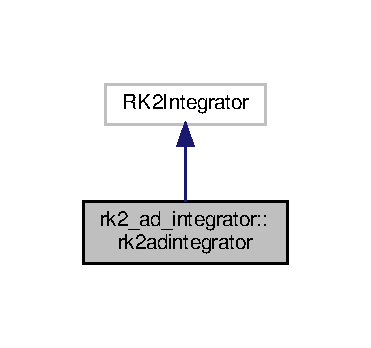
\includegraphics[width=178pt]{structrk2__ad__integrator_1_1rk2adintegrator__inherit__graph}
\end{center}
\end{figure}


Collaboration diagram for rk2\+\_\+ad\+\_\+integrator\+:\+:rk2adintegrator\+:\nopagebreak
\begin{figure}[H]
\begin{center}
\leavevmode
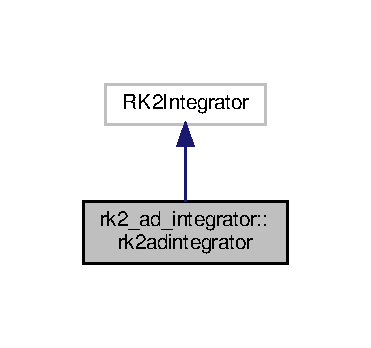
\includegraphics[width=178pt]{structrk2__ad__integrator_1_1rk2adintegrator__coll__graph}
\end{center}
\end{figure}


\subsection{Detailed Description}
Class for the Heun (R\+K2) AD integrator object. 

Definition at line 29 of file rk2\+\_\+ad\+\_\+integrator.\+f90.



The documentation for this type was generated from the following file\+:\begin{DoxyCompactItemize}
\item 
rk2\+\_\+ad\+\_\+integrator.\+f90\end{DoxyCompactItemize}

\hypertarget{structrk2__integrator_1_1rk2integrator}{}\section{rk2\+\_\+integrator\+:\+:rk2integrator Type Reference}
\label{structrk2__integrator_1_1rk2integrator}\index{rk2\+\_\+integrator\+::rk2integrator@{rk2\+\_\+integrator\+::rk2integrator}}


Class for the Heun (R\+K2) integrator object.  




Inheritance diagram for rk2\+\_\+integrator\+:\+:rk2integrator\+:\nopagebreak
\begin{figure}[H]
\begin{center}
\leavevmode
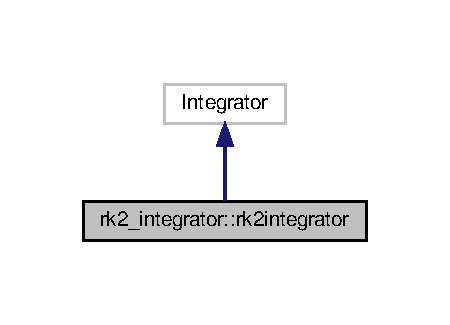
\includegraphics[width=216pt]{structrk2__integrator_1_1rk2integrator__inherit__graph}
\end{center}
\end{figure}


Collaboration diagram for rk2\+\_\+integrator\+:\+:rk2integrator\+:\nopagebreak
\begin{figure}[H]
\begin{center}
\leavevmode
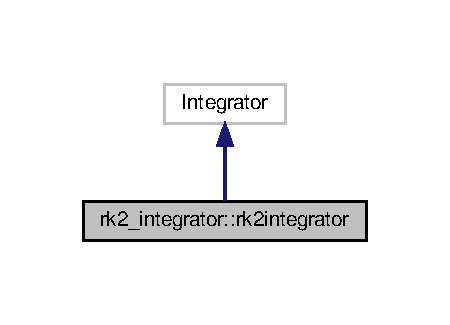
\includegraphics[width=216pt]{structrk2__integrator_1_1rk2integrator__coll__graph}
\end{center}
\end{figure}
\subsection*{Public Attributes}
\begin{DoxyCompactItemize}
\item 
\mbox{\Hypertarget{structrk2__integrator_1_1rk2integrator_abbcdfd65bf66491ba32a5df23a7241f7}\label{structrk2__integrator_1_1rk2integrator_abbcdfd65bf66491ba32a5df23a7241f7}} 
real(kind=8), dimension(\+:), allocatable \hyperlink{structrk2__integrator_1_1rk2integrator_abbcdfd65bf66491ba32a5df23a7241f7}{buf\+\_\+y1}
\begin{DoxyCompactList}\small\item\em Buffer to hold the intermediate position (Heun algorithm) \end{DoxyCompactList}\item 
\mbox{\Hypertarget{structrk2__integrator_1_1rk2integrator_a4b17658557f59d011a0fa185966d1c13}\label{structrk2__integrator_1_1rk2integrator_a4b17658557f59d011a0fa185966d1c13}} 
real(kind=8), dimension(\+:), allocatable \hyperlink{structrk2__integrator_1_1rk2integrator_a4b17658557f59d011a0fa185966d1c13}{buf\+\_\+f0}
\begin{DoxyCompactList}\small\item\em Buffer to hold tendencies at the initial position. \end{DoxyCompactList}\item 
\mbox{\Hypertarget{structrk2__integrator_1_1rk2integrator_a2daeb0252fa03949b85cff88f3d1c8ce}\label{structrk2__integrator_1_1rk2integrator_a2daeb0252fa03949b85cff88f3d1c8ce}} 
real(kind=8), dimension(\+:), allocatable \hyperlink{structrk2__integrator_1_1rk2integrator_a2daeb0252fa03949b85cff88f3d1c8ce}{buf\+\_\+f1}
\begin{DoxyCompactList}\small\item\em Buffer to hold tendencies at the intermediate position. \end{DoxyCompactList}\end{DoxyCompactItemize}


\subsection{Detailed Description}
Class for the Heun (R\+K2) integrator object. 

Definition at line 25 of file rk2\+\_\+integrator.\+f90.



The documentation for this type was generated from the following file\+:\begin{DoxyCompactItemize}
\item 
rk2\+\_\+integrator.\+f90\end{DoxyCompactItemize}

\hypertarget{structrk2__tl__integrator_1_1rk2tlintegrator}{}\section{rk2\+\_\+tl\+\_\+integrator\+:\+:rk2tlintegrator Type Reference}
\label{structrk2__tl__integrator_1_1rk2tlintegrator}\index{rk2\+\_\+tl\+\_\+integrator\+::rk2tlintegrator@{rk2\+\_\+tl\+\_\+integrator\+::rk2tlintegrator}}


Class for the Heun (R\+K2) TL integrator object.  




Inheritance diagram for rk2\+\_\+tl\+\_\+integrator\+:\+:rk2tlintegrator\+:\nopagebreak
\begin{figure}[H]
\begin{center}
\leavevmode
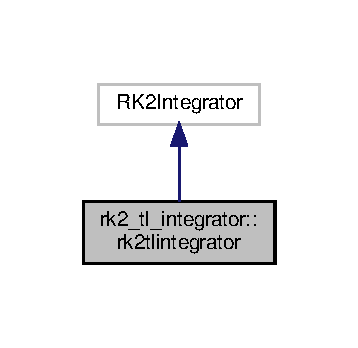
\includegraphics[width=172pt]{structrk2__tl__integrator_1_1rk2tlintegrator__inherit__graph}
\end{center}
\end{figure}


Collaboration diagram for rk2\+\_\+tl\+\_\+integrator\+:\+:rk2tlintegrator\+:\nopagebreak
\begin{figure}[H]
\begin{center}
\leavevmode
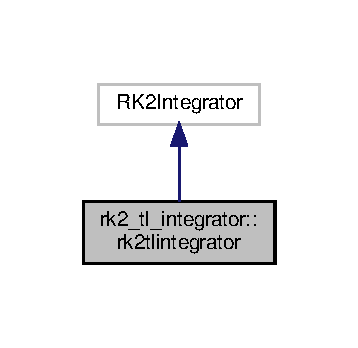
\includegraphics[width=172pt]{structrk2__tl__integrator_1_1rk2tlintegrator__coll__graph}
\end{center}
\end{figure}


\subsection{Detailed Description}
Class for the Heun (R\+K2) TL integrator object. 

Definition at line 29 of file rk2\+\_\+tl\+\_\+integrator.\+f90.



The documentation for this type was generated from the following file\+:\begin{DoxyCompactItemize}
\item 
rk2\+\_\+tl\+\_\+integrator.\+f90\end{DoxyCompactItemize}

\hypertarget{structrk4__ad__integrator_1_1rk4adintegrator}{}\section{rk4\+\_\+ad\+\_\+integrator\+:\+:rk4adintegrator Type Reference}
\label{structrk4__ad__integrator_1_1rk4adintegrator}\index{rk4\+\_\+ad\+\_\+integrator\+::rk4adintegrator@{rk4\+\_\+ad\+\_\+integrator\+::rk4adintegrator}}


Class for the fourth-\/order Runge-\/\+Kutta (R\+K4) AD integrator object.  




Inheritance diagram for rk4\+\_\+ad\+\_\+integrator\+:\+:rk4adintegrator\+:\nopagebreak
\begin{figure}[H]
\begin{center}
\leavevmode
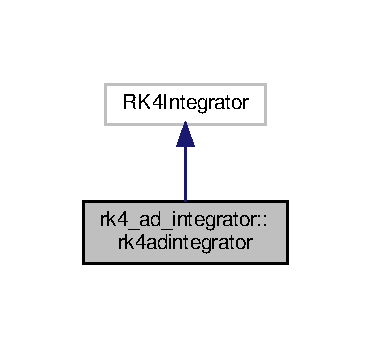
\includegraphics[width=178pt]{structrk4__ad__integrator_1_1rk4adintegrator__inherit__graph}
\end{center}
\end{figure}


Collaboration diagram for rk4\+\_\+ad\+\_\+integrator\+:\+:rk4adintegrator\+:\nopagebreak
\begin{figure}[H]
\begin{center}
\leavevmode
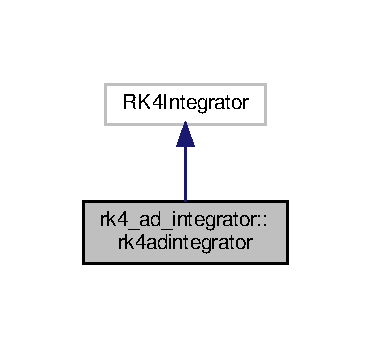
\includegraphics[width=178pt]{structrk4__ad__integrator_1_1rk4adintegrator__coll__graph}
\end{center}
\end{figure}


\subsection{Detailed Description}
Class for the fourth-\/order Runge-\/\+Kutta (R\+K4) AD integrator object. 

Definition at line 27 of file rk4\+\_\+ad\+\_\+integrator.\+f90.



The documentation for this type was generated from the following file\+:\begin{DoxyCompactItemize}
\item 
rk4\+\_\+ad\+\_\+integrator.\+f90\end{DoxyCompactItemize}

\hypertarget{structrk4__integrator_1_1rk4integrator}{}\section{rk4\+\_\+integrator\+:\+:rk4integrator Type Reference}
\label{structrk4__integrator_1_1rk4integrator}\index{rk4\+\_\+integrator\+::rk4integrator@{rk4\+\_\+integrator\+::rk4integrator}}


Class for the fourth-\/order Runge-\/\+Kutta (R\+K4) integrator object.  




Inheritance diagram for rk4\+\_\+integrator\+:\+:rk4integrator\+:\nopagebreak
\begin{figure}[H]
\begin{center}
\leavevmode
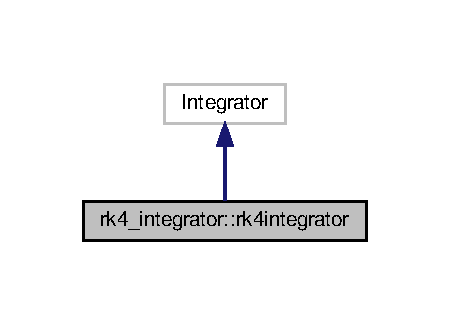
\includegraphics[width=216pt]{structrk4__integrator_1_1rk4integrator__inherit__graph}
\end{center}
\end{figure}


Collaboration diagram for rk4\+\_\+integrator\+:\+:rk4integrator\+:\nopagebreak
\begin{figure}[H]
\begin{center}
\leavevmode
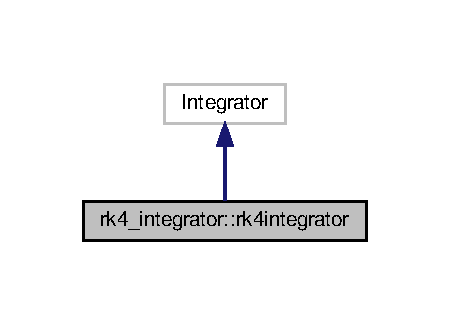
\includegraphics[width=216pt]{structrk4__integrator_1_1rk4integrator__coll__graph}
\end{center}
\end{figure}
\subsection*{Public Attributes}
\begin{DoxyCompactItemize}
\item 
\mbox{\Hypertarget{structrk4__integrator_1_1rk4integrator_ab6027434374b421735ea1a381f76b646}\label{structrk4__integrator_1_1rk4integrator_ab6027434374b421735ea1a381f76b646}} 
real(kind=8), dimension(\+:), allocatable \hyperlink{structrk4__integrator_1_1rk4integrator_ab6027434374b421735ea1a381f76b646}{buf\+\_\+y1}
\begin{DoxyCompactList}\small\item\em Buffer to hold the intermediate position. \end{DoxyCompactList}\item 
\mbox{\Hypertarget{structrk4__integrator_1_1rk4integrator_a3eb9cc4c7af5d63d7ade28b61b6e1715}\label{structrk4__integrator_1_1rk4integrator_a3eb9cc4c7af5d63d7ade28b61b6e1715}} 
real(kind=8), dimension(\+:), allocatable \hyperlink{structrk4__integrator_1_1rk4integrator_a3eb9cc4c7af5d63d7ade28b61b6e1715}{buf\+\_\+ka}
\begin{DoxyCompactList}\small\item\em Buffer to hold tendencies at the initial position. \end{DoxyCompactList}\item 
\mbox{\Hypertarget{structrk4__integrator_1_1rk4integrator_a0de0ebc4f37a48a1ae8bff0ff48d724b}\label{structrk4__integrator_1_1rk4integrator_a0de0ebc4f37a48a1ae8bff0ff48d724b}} 
real(kind=8), dimension(\+:), allocatable \hyperlink{structrk4__integrator_1_1rk4integrator_a0de0ebc4f37a48a1ae8bff0ff48d724b}{buf\+\_\+kb}
\begin{DoxyCompactList}\small\item\em Buffer to hold tendencies at the intermediate position. \end{DoxyCompactList}\end{DoxyCompactItemize}


\subsection{Detailed Description}
Class for the fourth-\/order Runge-\/\+Kutta (R\+K4) integrator object. 

Definition at line 23 of file rk4\+\_\+integrator.\+f90.



The documentation for this type was generated from the following file\+:\begin{DoxyCompactItemize}
\item 
rk4\+\_\+integrator.\+f90\end{DoxyCompactItemize}

\hypertarget{structrk4__tl__integrator_1_1rk4tlintegrator}{}\section{rk4\+\_\+tl\+\_\+integrator\+:\+:rk4tlintegrator Type Reference}
\label{structrk4__tl__integrator_1_1rk4tlintegrator}\index{rk4\+\_\+tl\+\_\+integrator\+::rk4tlintegrator@{rk4\+\_\+tl\+\_\+integrator\+::rk4tlintegrator}}


Class for the fourth-\/order Runge-\/\+Kutta (R\+K4) TL integrator object.  




Inheritance diagram for rk4\+\_\+tl\+\_\+integrator\+:\+:rk4tlintegrator\+:\nopagebreak
\begin{figure}[H]
\begin{center}
\leavevmode
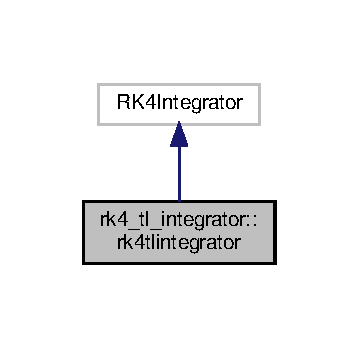
\includegraphics[width=172pt]{structrk4__tl__integrator_1_1rk4tlintegrator__inherit__graph}
\end{center}
\end{figure}


Collaboration diagram for rk4\+\_\+tl\+\_\+integrator\+:\+:rk4tlintegrator\+:\nopagebreak
\begin{figure}[H]
\begin{center}
\leavevmode
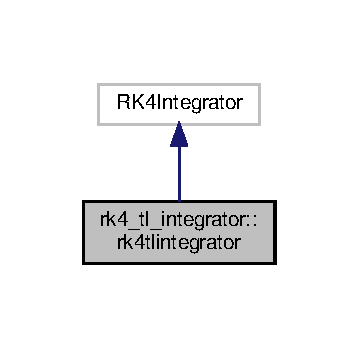
\includegraphics[width=172pt]{structrk4__tl__integrator_1_1rk4tlintegrator__coll__graph}
\end{center}
\end{figure}


\subsection{Detailed Description}
Class for the fourth-\/order Runge-\/\+Kutta (R\+K4) TL integrator object. 

Definition at line 27 of file rk4\+\_\+tl\+\_\+integrator.\+f90.



The documentation for this type was generated from the following file\+:\begin{DoxyCompactItemize}
\item 
rk4\+\_\+tl\+\_\+integrator.\+f90\end{DoxyCompactItemize}

\hypertarget{structstat_1_1stataccumulator}{}\section{stat\+:\+:stataccumulator Type Reference}
\label{structstat_1_1stataccumulator}\index{stat\+::stataccumulator@{stat\+::stataccumulator}}


Statistics accumulator objects class.  


\subsection*{Public Attributes}
\begin{DoxyCompactItemize}
\item 
\mbox{\Hypertarget{structstat_1_1stataccumulator_aa8f9105e658b823c19d9e7a67c1cb10b}\label{structstat_1_1stataccumulator_aa8f9105e658b823c19d9e7a67c1cb10b}} 
integer \hyperlink{structstat_1_1stataccumulator_aa8f9105e658b823c19d9e7a67c1cb10b}{i} =0
\begin{DoxyCompactList}\small\item\em Number of stats accumulated. \end{DoxyCompactList}\item 
\mbox{\Hypertarget{structstat_1_1stataccumulator_a6205ea1c87fe2aceaa1f5c554b33d3ab}\label{structstat_1_1stataccumulator_a6205ea1c87fe2aceaa1f5c554b33d3ab}} 
real(kind=8), dimension(\+:), allocatable \hyperlink{structstat_1_1stataccumulator_a6205ea1c87fe2aceaa1f5c554b33d3ab}{m}
\begin{DoxyCompactList}\small\item\em Vector storing the inline mean. \end{DoxyCompactList}\item 
\mbox{\Hypertarget{structstat_1_1stataccumulator_a6f1236b8cb1c59845c1551b170be33c4}\label{structstat_1_1stataccumulator_a6f1236b8cb1c59845c1551b170be33c4}} 
real(kind=8), dimension(\+:), allocatable \hyperlink{structstat_1_1stataccumulator_a6f1236b8cb1c59845c1551b170be33c4}{mprev}
\begin{DoxyCompactList}\small\item\em Previous mean vector. \end{DoxyCompactList}\item 
\mbox{\Hypertarget{structstat_1_1stataccumulator_a627af0d1895f670679a77742ac974c1c}\label{structstat_1_1stataccumulator_a627af0d1895f670679a77742ac974c1c}} 
real(kind=8), dimension(\+:), allocatable \hyperlink{structstat_1_1stataccumulator_a627af0d1895f670679a77742ac974c1c}{v}
\begin{DoxyCompactList}\small\item\em Vector storing the inline variance. \end{DoxyCompactList}\end{DoxyCompactItemize}


\subsection{Detailed Description}
Statistics accumulator objects class. 

Definition at line 20 of file stat.\+f90.



The documentation for this type was generated from the following file\+:\begin{DoxyCompactItemize}
\item 
stat.\+f90\end{DoxyCompactItemize}

\hypertarget{interfaceintegrator__def_1_1step__int}{}\section{integrator\+\_\+def\+:\+:step\+\_\+int Interface Reference}
\label{interfaceintegrator__def_1_1step__int}\index{integrator\+\_\+def\+::step\+\_\+int@{integrator\+\_\+def\+::step\+\_\+int}}


Abstract interface for the procedure to make the integrator compute a model\textquotesingle{}s time step.  




\subsection{Detailed Description}
Abstract interface for the procedure to make the integrator compute a model\textquotesingle{}s time step. 


\begin{DoxyParams}[1]{Parameters}
\mbox{\tt in,out}  & {\em integr} & Integrator object to perform the step with. \\
\hline
\mbox{\tt in}  & {\em y} & Initial point. \\
\hline
\mbox{\tt in}  & {\em t} & Actual integration time \\
\hline
\mbox{\tt out}  & {\em res} & Final point after the step. \\
\hline
\end{DoxyParams}


Definition at line 50 of file integrator\+\_\+def.\+f90.



The documentation for this interface was generated from the following file\+:\begin{DoxyCompactItemize}
\item 
integrator\+\_\+def.\+f90\end{DoxyCompactItemize}

\hypertarget{structtensor__def_1_1tensor}{}\section{tensor\+\_\+def\+:\+:tensor Type Reference}
\label{structtensor__def_1_1tensor}\index{tensor\+\_\+def\+::tensor@{tensor\+\_\+def\+::tensor}}


General class to represent a sparse tensor.  




Collaboration diagram for tensor\+\_\+def\+:\+:tensor\+:\nopagebreak
\begin{figure}[H]
\begin{center}
\leavevmode
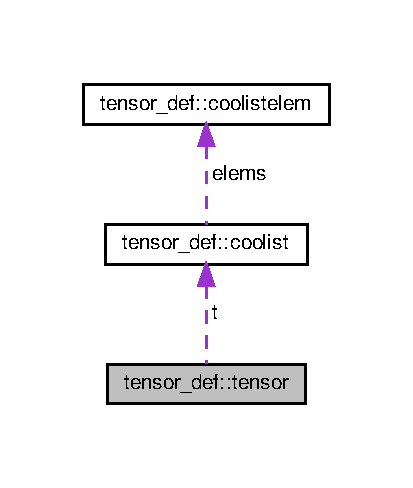
\includegraphics[width=198pt]{structtensor__def_1_1tensor__coll__graph}
\end{center}
\end{figure}
\subsection*{Public Attributes}
\begin{DoxyCompactItemize}
\item 
\mbox{\Hypertarget{structtensor__def_1_1tensor_a4f17ddd2ce1b8ee95414c9e0c395bfb7}\label{structtensor__def_1_1tensor_a4f17ddd2ce1b8ee95414c9e0c395bfb7}} 
type(\hyperlink{structtensor__def_1_1coolist}{coolist}), dimension(\+:), allocatable \hyperlink{structtensor__def_1_1tensor_a4f17ddd2ce1b8ee95414c9e0c395bfb7}{t}
\begin{DoxyCompactList}\small\item\em Sparse representation of the tensor as a \hyperlink{structtensor__def_1_1coolist}{tensor\+\_\+def\+::coolist} . \end{DoxyCompactList}\end{DoxyCompactItemize}


\subsection{Detailed Description}
General class to represent a sparse tensor. 

Definition at line 36 of file tensor\+\_\+def.\+f90.



The documentation for this type was generated from the following file\+:\begin{DoxyCompactItemize}
\item 
tensor\+\_\+def.\+f90\end{DoxyCompactItemize}

\hypertarget{structtl__ad__tensor_1_1tltensor}{}\section{tl\+\_\+ad\+\_\+tensor\+:\+:tltensor Type Reference}
\label{structtl__ad__tensor_1_1tltensor}\index{tl\+\_\+ad\+\_\+tensor\+::tltensor@{tl\+\_\+ad\+\_\+tensor\+::tltensor}}


Tensor representation of the Tangent Linear tendencies.  




Collaboration diagram for tl\+\_\+ad\+\_\+tensor\+:\+:tltensor\+:\nopagebreak
\begin{figure}[H]
\begin{center}
\leavevmode
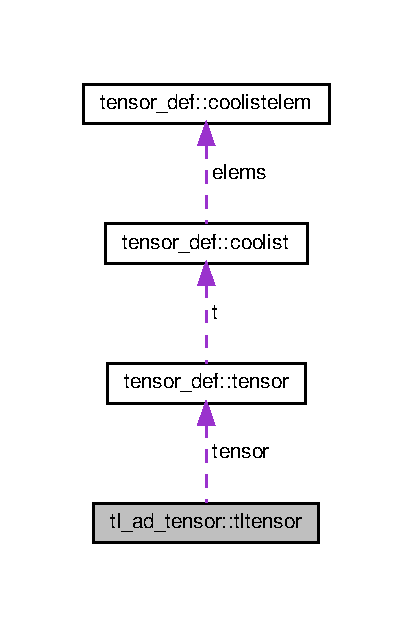
\includegraphics[width=198pt]{structtl__ad__tensor_1_1tltensor__coll__graph}
\end{center}
\end{figure}
\subsection*{Public Attributes}
\begin{DoxyCompactItemize}
\item 
\mbox{\Hypertarget{structtl__ad__tensor_1_1tltensor_a4ce89c8dccec756a7964b381719b95a5}\label{structtl__ad__tensor_1_1tltensor_a4ce89c8dccec756a7964b381719b95a5}} 
type(\hyperlink{structtensor__def_1_1tensor}{tensor}) \hyperlink{structtl__ad__tensor_1_1tltensor_a4ce89c8dccec756a7964b381719b95a5}{tensor}
\begin{DoxyCompactList}\small\item\em The TL tensor object. \end{DoxyCompactList}\item 
\mbox{\Hypertarget{structtl__ad__tensor_1_1tltensor_af957e83eded70844c88f2b8d5df30b25}\label{structtl__ad__tensor_1_1tltensor_af957e83eded70844c88f2b8d5df30b25}} 
integer, dimension(\+:), allocatable \hyperlink{structtl__ad__tensor_1_1tltensor_af957e83eded70844c88f2b8d5df30b25}{count\+\_\+elems}
\begin{DoxyCompactList}\small\item\em A list of the number of non-\/zero entries of the tensor component along the first index. \end{DoxyCompactList}\end{DoxyCompactItemize}


\subsection{Detailed Description}
Tensor representation of the Tangent Linear tendencies. 

Definition at line 34 of file tl\+\_\+ad\+\_\+tensor.\+f90.



The documentation for this type was generated from the following file\+:\begin{DoxyCompactItemize}
\item 
tl\+\_\+ad\+\_\+tensor.\+f90\end{DoxyCompactItemize}

%--- End generated contents ---

% Index
\backmatter
\newpage
\phantomsection
\clearemptydoublepage
\addcontentsline{toc}{chapter}{Index}
\printindex

\end{document}
